\noindent Eines der zentralen Ziele von Design For Six Sigma besteht darin, Ursachen-Wirkungs-Beziehungen zu ermitteln, um Produkte und Prozesse bestm\"{o}glich zu verstehen. Zur Beschreibung des Zusammenhangs von Eingangs-, St\"{o}r- und Zielgr\"{o}{\ss}en werden unterschiedliche Methoden angewendet: 

\begin{itemize}
    \item Analytische BerechnungAuf Basis eines Systemmodells werden die Zielgr\"{o}{\ss}en als Funktion der Eingangsgr\"{o}{\ss}en berechnet. Notwendig ist ein physikalisches Verhaltensmodell, das das Systemverhalten mit einer ausreichenden Pr\"{a}zision beschreibt.
    \item  SimulationEine Simulation wird durchgef\"{u}hrt, wenn das Modell zwar grunds\"{a}tzlich bekannt ist, die analytische Berechnung aber aufgrund der komplexen Geometrie oder den Randbedingungen un\"{u}bersichtlich und aufwendig wird.
    \item  ExperimentMit Experimenten werden die Simulationen und Berechnungen best\"{a}tigt. Mit dem Hintergrundwissen zum Modellverhalten, das aus der analytischen Rechnung und der Simulation kommt, kann der experimentelle Aufwand klein gehalten werden. 
\end{itemize}

\noindent Der Zusammenhang zwischen den unterschiedlichen Methoden zur Modellierung eines Systems ist in Bild \ref{fig:Modell} zusammenfassend dargestellt.

\noindent 
\begin{figure}[H]
  \centerline{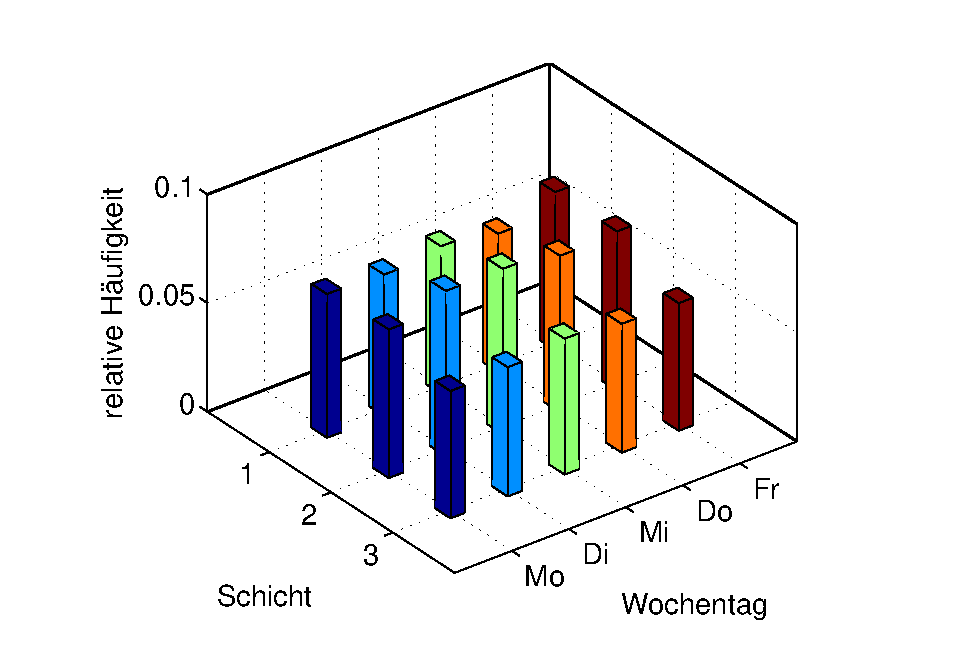
\includegraphics[width=0.6\textwidth]{Kapitel12/Bilder/image1}}
  \caption{Gegen\"{u}berstellung von analytischer Berechnung, numerischer Simulation und Experiment}
  \label{fig:Modell}
\end{figure}

\noindent Insbesondere die Simulation, aber auch die analytische Berechnung erfordern ein Modell des abzubildenden Systems oder Prozesses. Es werden mathematische und physikalische Modelle unterschieden, beide werden in Bild \ref{fig:Modell} gegen\"{u}bergestellt.

\clearpage

\noindent a) Physikalisches Systemmodell 

\noindent 
\begin{figure}[H]
  \centerline{\includegraphics[width=0.5\textwidth]{Kapitel12/Bilder/image2-1}}
\end{figure}

b) Mathematisches Systemmodell

\noindent 
\begin{figure}[H]
  \centerline{\includegraphics[width=0.5\textwidth]{Kapitel12/Bilder/image2-2}}
  \caption{Vergleich von physikalischen und mathematischen Systemmodellen}
  \label{fig:BlackboxModell}
\end{figure}

\noindent W\"{a}hrend in der klassischen Modellbildung das physikalische Modell analytisch hergeleitet wird, wird im Rahmen der mathematischen Modellbildung das zu untersuchende System als Black-Box betrachtet. Dieser Ansatz f\"{u}hrt zu einem Modell, bei dem das Zusammenwirken der Ein- und Zielgr\"{o}{\ss}en mathematisch \"{u}ber sogenannte Regressionsfunktionen beschrieben wird.\newline

\noindent In diesem Kapitel werden zun\"{a}chst Regressionsfunktionen f\"{u}r zweidimensionale Datens\"{a}tze berechnet und ihr Konfidenzbereich ermittelt. Dabei werden lineare und nichtlineare Regressionen betrachtet. In Kapitel \ref{twelve} wird das Vorgehen auf M-dimensionale Datens\"{a}tze verallgemeinert.

\subsection{Lineare Regression}

\noindent Anhand der linearen Regression zweidimensionaler Datens\"{a}tze werden die Grundprinzipien der Regression und die wesentlichen statistischen Verfahren zur Bewertung der Regressionsfunktion vorgestellt. Liegt eine Beobachtung mit einer Stichprobe

\begin{equation}\label{eq:twelveone}
(x_{1} ,y_{1}),(x_{2} ,y_{2} ), ...,(x_{N} ,y_{N})
\end{equation}

\noindent aus einer zweidimensionalen Grundgesamtheit vor, k\"{o}nnen diese Punkte oftmals in guter N\"{a}herung durch eine Geradengleichung der Form

\begin{equation}\label{eq:twelvetwo}
y(x)=b_{0} +b_{1} \cdot x
\end{equation}

\noindent beschrieben werden kann. Der Parameter $b_{0}$ beschreibt den Schnittpunkt mit der y-Achse, w\"{a}hrend der Parameter $b_{1}$ die Steigung der Geraden beschreibt. Der durch die Funktion gesch\"{a}tzte Wert wird mit y(x) bezeichnet.

\clearpage

\noindent
\colorbox{lightgray}{%
\arrayrulecolor{white}%
\renewcommand\arraystretch{0.6}%
\begin{tabular}{ wl{16.5cm} }
{\fontfamily{phv}\selectfont
\noindent{Beispiel: Temperatursensor}}
\end{tabular}%
}\bigskip

\noindent Die Ausgangssituation wird an einem Beispiel verdeutlicht, bei dem der Zusammenhang zwischen der Temperatur eines Motor\"{o}ls und der Ausgangsspannung eines Temperatursensors beschrieben werden soll. Die aufgenommenen Stichprobenwerte sind in Tabelle \ref{tab:twelveone} aufgelistet. 

\begin{table}[H]
\setlength{\arrayrulewidth}{.1em}
\caption{Zusammenhang zwischen \"{O}ltemperatur und Ausgangsspannung eines Temperatursensors}
\setlength{\fboxsep}{0pt}%
\colorbox{lightgray}{%
\arrayrulecolor{white}%
\begin{tabular}{ wc{3.7cm} | wc{1.75cm} | wc{1.72cm} | wc{1.72cm} | wc{1.72cm} | wc{1.75cm} | wc{1.72cm} }
\hline\xrowht{10pt}

\fontfamily{phv}\selectfont\textbf{Temperatur T / $^\circ$C} &
\fontfamily{phv}\selectfont{0} &
\fontfamily{phv}\selectfont{10} &
\fontfamily{phv}\selectfont{20} &
\fontfamily{phv}\selectfont{30} &
\fontfamily{phv}\selectfont{40} &
\fontfamily{phv}\selectfont{50} \\ \hline \xrowht{10pt}

\fontfamily{phv}\selectfont\textbf{Spannung U / V} &
\fontfamily{phv}\selectfont{2.766} &
\fontfamily{phv}\selectfont{2.862} &
\fontfamily{phv}\selectfont{3.005} &
\fontfamily{phv}\selectfont{3.120} &
\fontfamily{phv}\selectfont{3.173} &
\fontfamily{phv}\selectfont{3.411} \\ \hline \xrowht{10pt}

\fontfamily{phv}\selectfont\textbf{Temperatur T / $^\circ$C} &
\fontfamily{phv}\selectfont{60} &
\fontfamily{phv}\selectfont{70} &
\fontfamily{phv}\selectfont{80} &
\fontfamily{phv}\selectfont{90} &
\fontfamily{phv}\selectfont{100} &
 \\ \hline \xrowht{10pt}

\fontfamily{phv}\selectfont\textbf{Spannung U / V} &
\fontfamily{phv}\selectfont{3.676} &
\fontfamily{phv}\selectfont{3.803} &
\fontfamily{phv}\selectfont{3.944} &
\fontfamily{phv}\selectfont{4.188} &
\fontfamily{phv}\selectfont{4.165} &
\\ \hline

\end{tabular}%
}
\label{tab:twelveone}
\end{table}

\noindent In Bild \ref{fig:RegressionLinearOeltemperatur} wird die Stichprobe als Streudiagramm visualisiert. Der funktionale Zusammenhang zwischen der \"{O}ltemperatur und der Ausgangsspannung des Temperatursensors kann in diesem Fall \"{u}ber eine Gerade approximiert werden. Hierzu ist in Bild \ref{fig:RegressionLinearOeltemperatur} zus\"{a}tzlich die entsprechende Regressionsgerade eingezeichnet.

\noindent 
\begin{figure}[H]
  \centerline{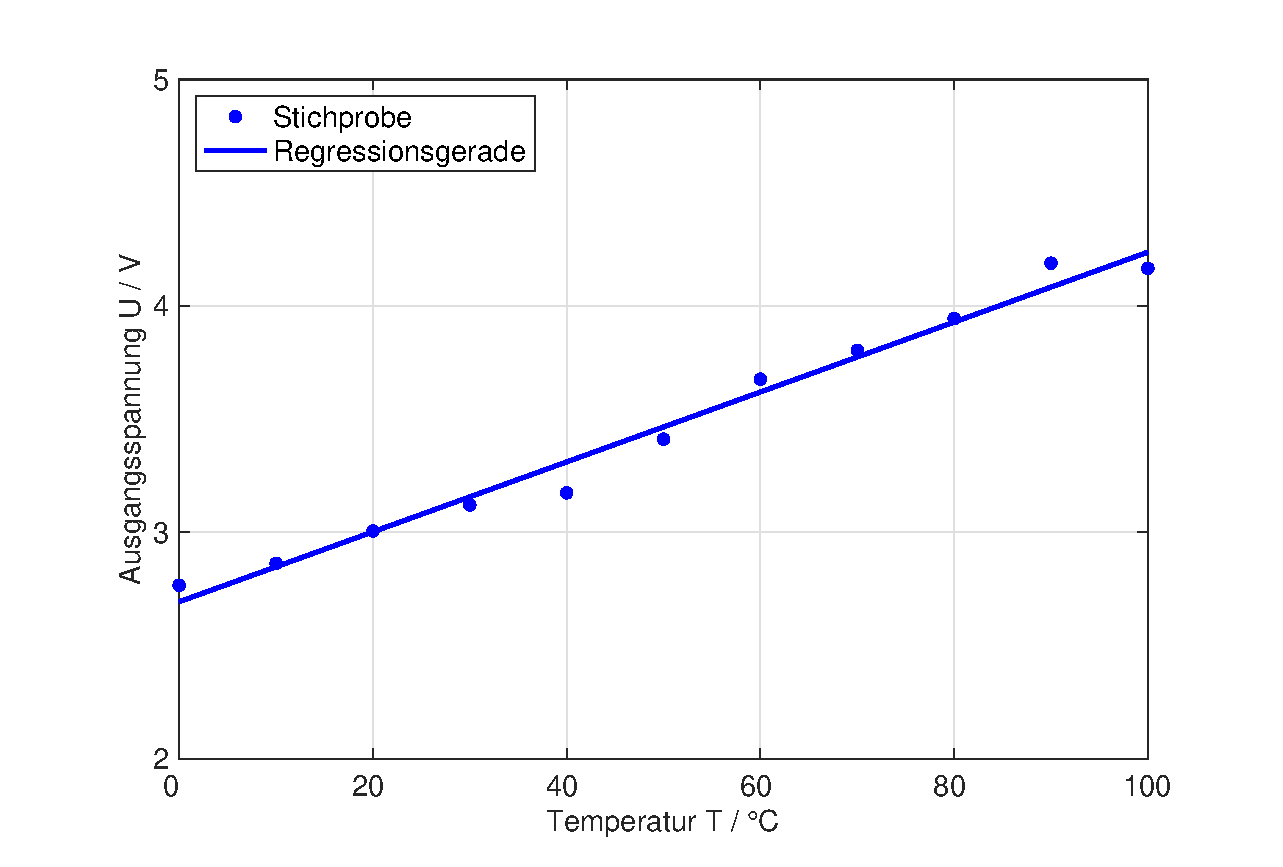
\includegraphics[width=0.5\textwidth]{Kapitel12/Bilder/image3}}
  \caption{Grafische Darstellung der Stichprobe und der entsprechenden Regressionsgerade f\"{u}r den Zusammenhang zwischen der \"{O}ltemperatur und der Ausgangsspannung des Temperatursensors}
  \label{fig:RegressionLinearOeltemperatur}
\end{figure}

\noindent Die Punkte in Bild \ref{fig:RegressionLinearOeltemperatur} liegen nicht pr\"{a}zise auf einer Linie, sodass das Einzeichnen einer Geraden zun\"{a}chst nicht eindeutig ist. Um insbesondere bei gro{\ss}en Datenmengen eine Funktion eindeutig berechnen zu k\"{o}nnen, wurde von Gau{\ss} das Prinzip der kleinsten Quadrate entwickelt. Nach diesem Prinzip ist die Gerade so zu legen, dass die Summe der Quadrate aller Abst\"{a}nde von den Stichprobenwerten zu der Geraden m\"{o}glichst klein wird. Die durch dieses Verfahren bestimmte Funktion wird als Regressionsfunktion bezeichnet. Der Abstand der Stichprobenwerte von der Regressionsgeraden wird als Residuum bezeichnet. \ref{fig:RegressionLinearOeltemperatur2} verdeutlicht den Begriff des Residuums.

\noindent 
\begin{figure}[H]
  \centerline{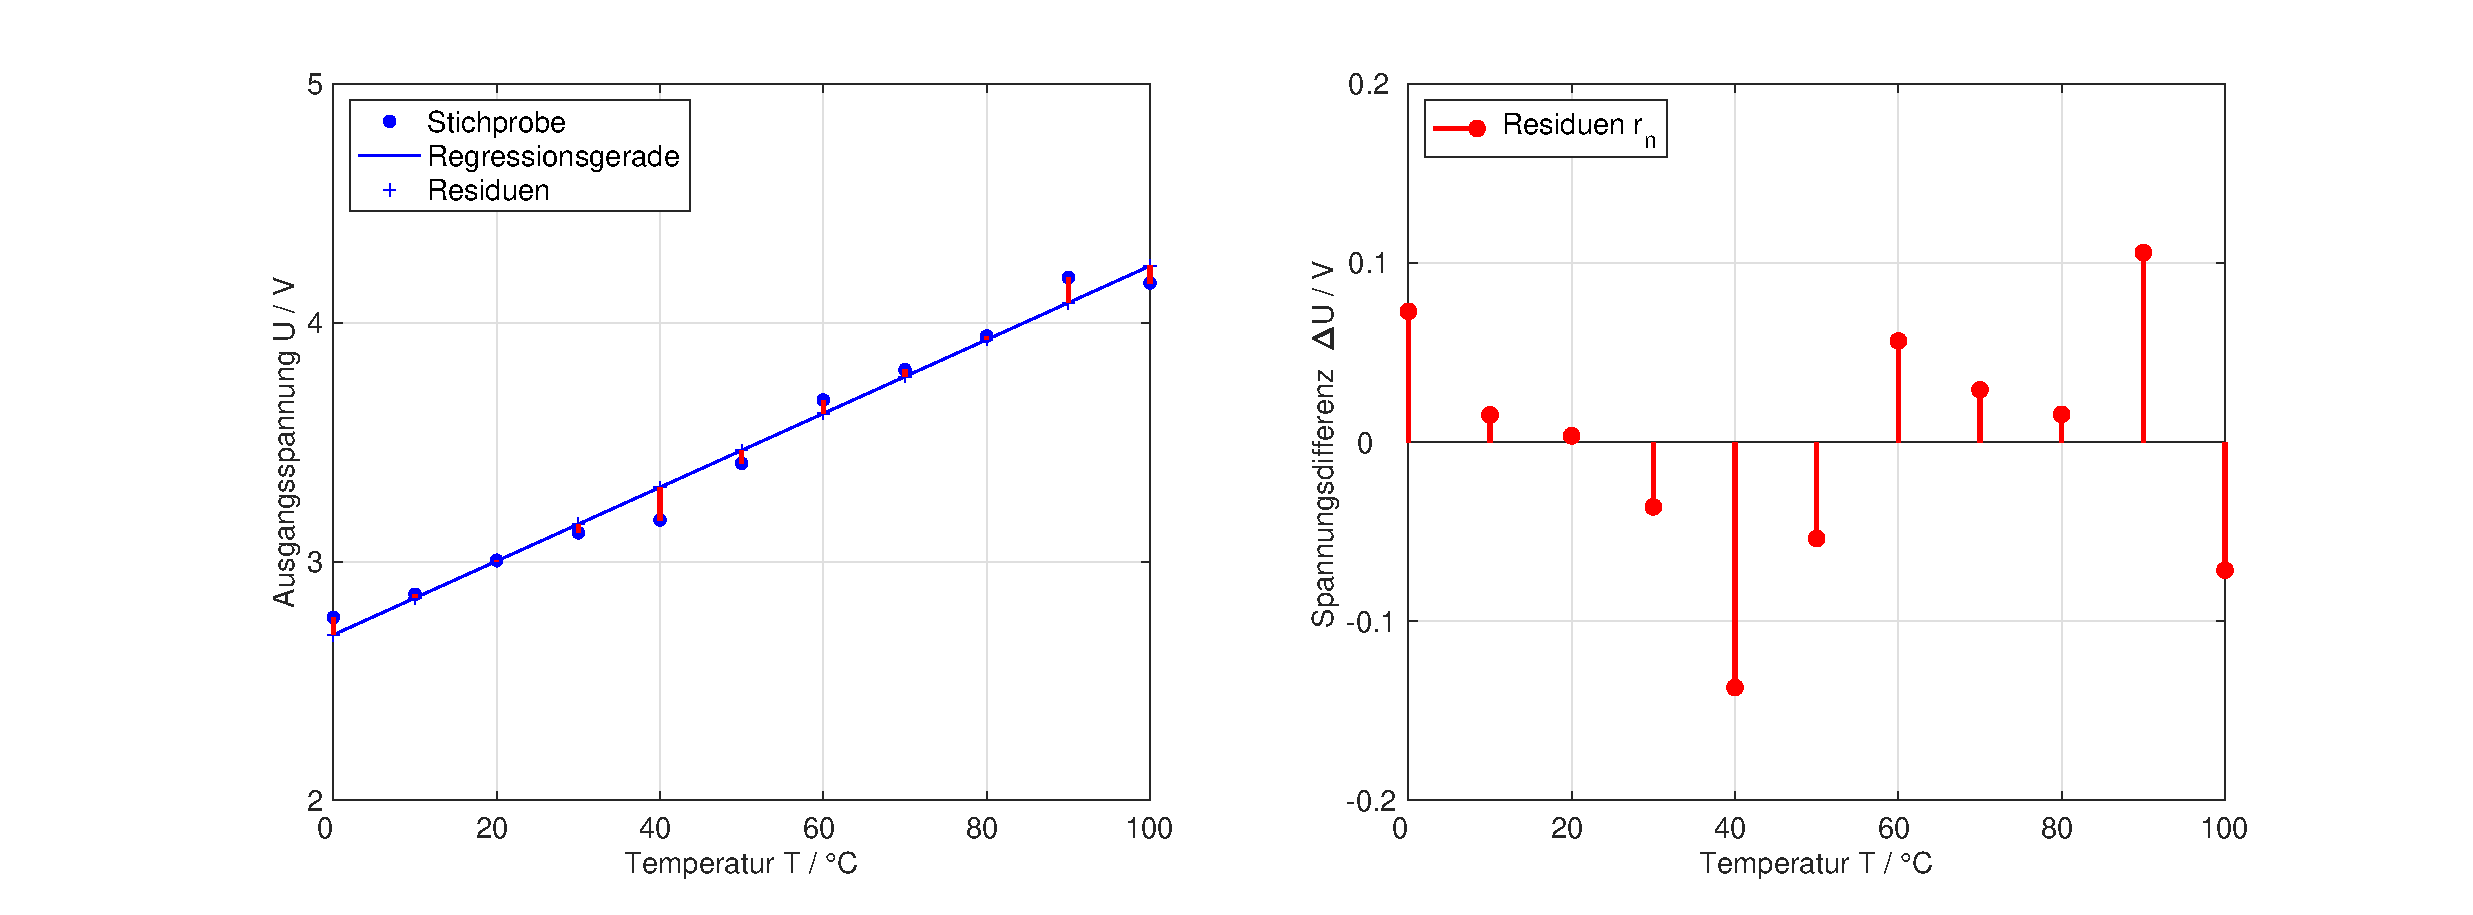
\includegraphics[width=1\textwidth]{Kapitel12/Bilder/image4}}
  \caption{Grafische Darstellung des Abstandes der Stichprobenwerte von der Regressionsgeraden (Residuen $r_{n}$)}
  \label{fig:RegressionLinearOeltemperatur2}
\end{figure}

\noindent Wird die Regressionsgerade \"{u}ber die Gleichung

\begin{equation}\label{eq:twelvethree}
y(x)=b_{0} +b_{1} \cdot x
\end{equation}

\noindent beschrieben, ergibt sich f\"{u}r das Wertepaar ($x_{n}$, $y_{n}$) sich das Residuum $r_{n}$ zu

\begin{equation}\label{eq:twelvefour}
r_{n} =y_{n} -y(x_{n} )=y_{n} -(b_{0} +b_{1} \cdot x_{n})
\end{equation}

\noindent Die Parameter $b_{0}$ und $b_{1}$ sollen so bestimmt werden, dass die Summe der Abstandsquadrate a minimal wird. Die Summe der Abstandsquadrate a errechnet sich zu

\begin{equation}\label{eq:twelvefive}
a=\sum _{n=1}^{N}r_{n}^{2}  =\sum _{n=1}^{N}\left(y_{n} -b_{0} -b_{1} \cdot x_{n} \right)^{2}
\end{equation}

\noindent Damit diese Funktion ein Minimum aufweist, m\"{u}ssen die partiellen Ableitungen von a nach den Parametern $b_{m}$ der Regressionsfunktion verschwinden. Damit ergeben sich die notwendigen Bedingungen

\begin{equation}\label{eq:twelvesix}
\dfrac{\partial a}{\partial b_{1}} =0
\end{equation}

\noindent und 

\begin{equation}\label{eq:twelveseven}
\dfrac{\partial a}{\partial b_{0}} =0
\end{equation}

\noindent Die Ableitungen aus Gleichung \eqref{eq:twelvesix} und Gleichung \eqref{eq:twelveseven} berechnen sich zu

\begin{equation}\label{eq:twelveeight}
\dfrac{\partial a}{\partial b_{1}} =-2\cdot \sum _{n=1}^{N}\left(x_{n} \cdot (y_{n} -b_{0} -b_{1} \cdot x_{n})\right)
\end{equation}

\noindent und

\begin{equation}\label{eq:twelvenine}
\dfrac{\partial a}{\partial b_{0} } =-2\cdot \sum _{n=1}^{N}\left(y_{n} -b_{0} -b_{1} \cdot x_{n} \right)
\end{equation}

\noindent Beide Ausdr\"{u}cke werden zu null gesetzt, und es ergeben sich die Gleichungen

\begin{equation}\label{eq:twelveten}
0=\sum _{n=1}^{N}x_{n} \cdot \left(y_{n} -b_{0} -b_{1} \cdot x_{n} \right) =\sum _{n=1}^{N}x_{n} \cdot y_{n}  -b_{0} \cdot \sum _{n=1}^{N}x_{n}  -b_{1} \cdot \sum _{n=1}^{N}x_{n}^{2}
\end{equation}

\noindent und 

\begin{equation}\label{eq:twelveeleven}
0=\sum _{n=1}^{N}\left(y_{n} -b_{0} -b_{1} \cdot x_{n} \right) =\sum _{n=1}^{N}y_{n}  -\sum _{n=1}^{N}b_{0}  -b_{1} \cdot \sum _{n=1}^{N}x_{n}  =\sum _{n=1}^{N}y_{n}  -N\cdot b_{0} -b_{1} \cdot \sum _{n=1}^{N}x_{n}
\end{equation}

\noindent Unter Ber\"{u}cksichtigung der Definition f\"{u}r den Mittelwert

\begin{equation}\label{eq:twelvetwelve}
\bar{x}=\dfrac{1}{N} \cdot \left(x_{1} +x_{2} +...+x_{N} \right)=\dfrac{1}{N} \cdot \sum _{n=1}^{N}x_{n}
\end{equation}

\noindent beziehungsweise 

\begin{equation}\label{eq:twelvethirteen}
\bar{y}=\dfrac{1}{N} \cdot \left(y_{1} +y_{2} +...+y_{N} \right)=\dfrac{1}{N} \cdot \sum _{n=1}^{N}y_{n}
\end{equation}

\noindent ergibt sich aus Gleichung \eqref{eq:twelveten}

\begin{equation}\label{eq:twelvefourteen}
b_{0} \cdot N\cdot \bar{x}+b_{1} \cdot \sum _{n=1}^{N}x_{n}^{2}  =\sum _{n=1}^{N}x_{n} \cdot y_{n}
\end{equation}

\noindent und aus Gleichung \eqref{eq:twelvetwelve} folgt

\begin{equation}\label{eq:twelvefifteen}
b_{0} +b_{1} \cdot \bar{x}=\bar{y}
\end{equation}

\noindent Dieses Gleichungssystem kann nach $b_{1}$ und $b_{0}$ aufgel\"{o}st werden. Mit den Ausdr\"{u}cken f\"{u}r die Varianz

\begin{equation}\label{eq:twelvesixteen}
s_{x}^{2} =\dfrac{1}{N-1} \cdot \sum _{n=1}^{N}\left(x_{n} -\bar{x}\right)^{2}  =\dfrac{1}{N-1} \cdot \left(\sum _{n=1}^{N}x_{n}^{2}  -N\cdot \bar{x}^{2} \right)
\end{equation}

\noindent und die Kovarianz 

\begin{equation}\label{eq:twelveseventeen}
s_{xy} =\dfrac{1}{N-1} \cdot \sum _{n=1}^{N}\left(\left(x_{n} -\bar{x}\right)\cdot \left(y_{n} -\bar{y}\right)\right) =\dfrac{1}{N-1} \cdot \left(\sum _{n=1}^{N}x_{n} \cdot y_{n}  -N\cdot \bar{x}\cdot \bar{y}\right)
\end{equation}

\noindent k\"{o}nnen sie umgeformt werden zu

\begin{equation}\label{eq:twelveeighteen}
b_{1} =\dfrac{\sum _{n=1}^{N}x_{n} \cdot y_{n}  -N\cdot \bar{x}\cdot \bar{y}}{\sum _{n=1}^{N}x_{n}^{2}  -N\cdot \bar{x}^{2} } =\dfrac{s_{xy} }{s_{x}^{2} }
\end{equation}

\noindent und 

\begin{equation}\label{eq:twelvenineteen}
b_{0} =\bar{y}-b_{1} \cdot \bar{x}
\end{equation}

\noindent Damit ergibt sich die Geradengleichung

\begin{equation}\label{eq:twelvetwenty}
y(x)-\bar{y}=b_{1} \cdot (x-\bar{x})
\end{equation}

\noindent und die Summe aller Residuen errechnet sich zu

\begin{equation}\label{eq:twelvetwentyone}
\begin{split}
\sum _{n=1}^{N}r_{n} & = \sum _{n=1}^{N}\left(y_{n} -y(x_{n})\right) =\sum _{n=1}^{N}\left(y_{n} -b_{1} \cdot (x_{n} -\bar{x})-\bar{y}\right) =\sum _{n=1}^{N}\left(y_{n} -b_{1} \cdot x_{n} +b_{1} \cdot \bar{x}-\bar{y}\right) \\ 
& =  \sum _{n=1}^{N}y_{n}-b_{1}\cdot \sum _{n=1}^{N}x_{n}+b_{1}\cdot N \cdot \bar{x}-N\cdot \bar{y} = N\cdot \bar{y} - b_{1}\cdot N\cdot \bar{x}+ b_{1}\cdot N\cdot \bar{x} -N\cdot \bar{y}=0
\end{split}
\end{equation}

\noindent F\"{u}r das Beispiel des \"{O}ltemperatursensors aus Tabelle 11.1 ergeben sich die Koeffizienten $b_{1}$ und $b_{0}$ zu 

\begin{equation}\label{eq:twelvetwentytwo}
b_{1} =\dfrac{\sum _{n=1}^{N}x_{n} \cdot y_{n} -N\cdot \bar{x}\cdot \bar{y}}{\sum _{n=1}^{N}x_{n}^{2} -N\cdot \bar{x}^{2}} =\dfrac{s_{xy}}{s_{x}^{2}} =0.0154
\end{equation}

\noindent und 

\begin{equation}\label{eq:twelvetwentythree}
b_{0} =\bar{y}-b_{1} \cdot \bar{x}=2.693
\end{equation}

\noindent Die entsprechende Gerade ist bereits in Bild \ref{fig:RegressionLinearOeltemperatur} und Bild \ref{fig:RegressionLinearOeltemperatur2} eingezeichnet.

\noindent Das Verfahren zur Berechnung einer Regressionsgeraden auf Basis einer Stichprobe ist in Tabelle \ref{tab:twelvetwo} zusammengefasst.

\clearpage

\begin{table}[H]
\setlength{\arrayrulewidth}{.1em}
\caption{Vorgehen zur Bestimmung des Parameters $b_{1}$ und $b_{0}$ einer Regressionsgeraden}
\setlength{\fboxsep}{0pt}%
\colorbox{lightgray}{%
\arrayrulecolor{white}%
\begin{tabular}{| wc{1cm} | wc{15.5cm} }
\xrowht{15pt}

\fontfamily{phv}\selectfont\textbf{Nr.} & 
\fontfamily{phv}\selectfont\textbf{Prozessschritt}\\ \hline \xrowht{20pt}

\multirow{4}{*}{\fontfamily{phv}\selectfont{1}} &
\fontfamily{phv}\selectfont{Berechnen der Mittelwerte aus der Stichprobe} \\\xrowht{25pt}
& \fontfamily{phv}\selectfont{$\bar{x}=\dfrac{1}{N} \cdot \sum _{n=1}^{N}x_{n}  \qquad \qquad \qquad \qquad $ und $\qquad  \qquad  \qquad \qquad \bar{y}=\dfrac{1}{N} \cdot \sum _{n=1}^{N}y_{n}$}  \\ \hline \xrowht{20pt}

\multirow{4}{*}{\fontfamily{phv}\selectfont{2}} &
\fontfamily{phv}\selectfont{Berechnen der Varianz und der Kovarianz aus der Stichprobe} \\\xrowht{25pt}
& \fontfamily{phv}\selectfont{$s_{x}^{2} =\dfrac{1}{N-1} \cdot \sum _{n=1}^{N}(x_{n} -\bar{x})^{2}  \qquad \qquad \qquad  $ und $\qquad \quad \qquad s_{xy} =\dfrac{1}{N-1} \cdot \sum _{n=1}^{N}(x_{n} -\bar{x})\cdot (y_{n} -\bar{y})$}  \\ \hline \xrowht{20pt}

\multirow{4}{*}{\fontfamily{phv}\selectfont{3}} &
\fontfamily{phv}\selectfont{Berechnen der Parameter b0 und b1 der Regressionsgeraden} \\\xrowht{25pt}
& \fontfamily{phv}\selectfont{$b_{1} =\dfrac{s_{xy} }{s_{x}^{2} } \qquad \qquad \qquad \qquad $ und $\qquad  \qquad  \qquad \qquad b_{0} =\bar{y}-b_{1} \cdot \bar{x}$}  \\ \hline \xrowht{20pt}

\multirow{4}{*}{\fontfamily{phv}\selectfont{4}} &
\fontfamily{phv}\selectfont{Beschreiben der Stichprobe mit der Regressionsfunktion} \\\xrowht{25pt}
& \fontfamily{phv}\selectfont{$y\left(x\right)=b_{1} \cdot x+b_{0} =b_{1} \cdot \left(x-\bar{x}\right)+\bar{y}$}  \\ \hline

\end{tabular}%
}\bigskip
\label{tab:twelvetwo}
\end{table}

\noindent Damit ist das Vorgehen zur Festlegung der Regressionsgeraden einer Stichprobe festgelegt. F\"{u}r diese Stichprobe ist die berechnete Gerade im Sinne der Summe der Fehlerquadrate die bestm\"{o}gliche L\"{o}sung. Wie bei der Bestimmung der Konfidenzintervalle bleibt aber zun\"{a}chst die Frage offen, inwieweit die bestimmte Geradengleichung die Grundgesamtheit wiedergibt.

\subsubsection{Modell zur statistischen Bewertung der Regression}

\noindent Zur statistischen Bewertung der Regression wird die Grundgesamtheit der Zielgr\"{o}{\ss}e beschrieben als

\begin{equation}\label{eq:twelvetwentyfour}
y=\beta _{0} +\beta _{1} \cdot x+e
\end{equation}

\noindent Dabei ist die Gr\"{o}{\ss}e x die Eingangsgr\"{o}{\ss}e, f\"{u}r die die Zielgr\"{o}{\ss}e y bestimmt werden soll. Sie wird nicht durch den Prozess festgelegt und besitzt damit keine Streuung. Die Messwerte unterliegen einem Messfehler. F\"{u}r den Messfehler wird davon ausgegangen, dass er normalverteilt ist. Er weist einen Erwartungswert von 

\begin{equation}\label{eq:twelvetwentyfive}
E(e)=\mu _{e} =0
\end{equation}

\noindent und eine Varianz 

\begin{equation}\label{eq:twelvetwentysix}
\left((e-\mu _{e})^{2} \right)=\sigma ^{2}
\end{equation}

\noindent auf. Bild \ref{fig:AnsatzHerleitungKonfidenzbereich} stellt die Annahmen zur statistischen Bewertung der Regression grafisch dar.

\clearpage

\noindent 
\begin{figure}[H]
  \centerline{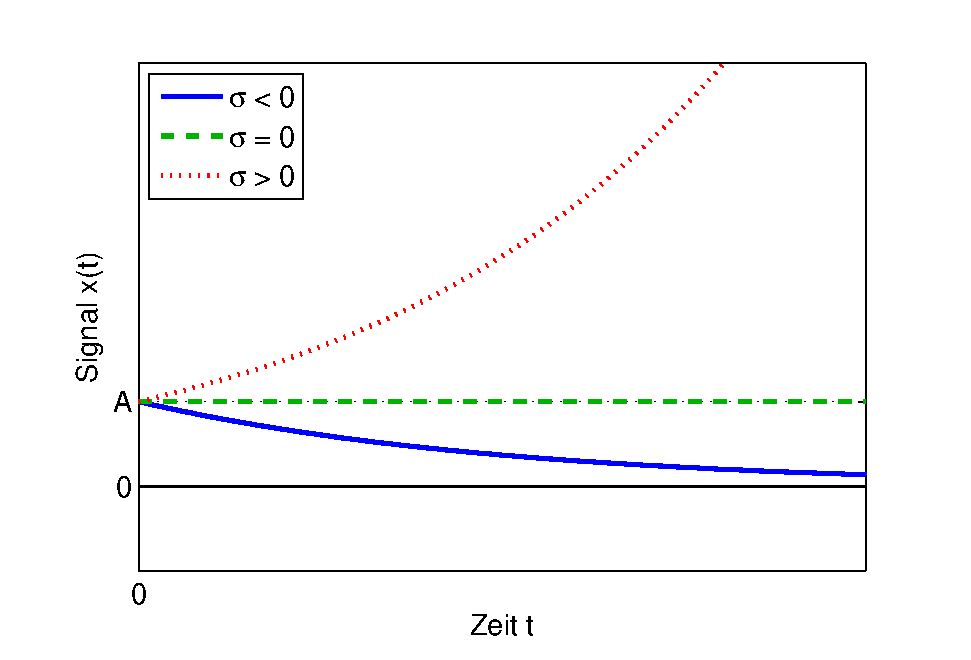
\includegraphics[width=0.5\textwidth]{Kapitel12/Bilder/image5}}
  \caption{Grafische Darstellung der Annahmen zur Bewertung der Regressionskoeffizienten}
  \label{fig:AnsatzHerleitungKonfidenzbereich}
\end{figure}

\noindent Damit hat die Zielgr\"{o}{\ss}e y den Erwartungswert 

\begin{equation}\label{eq:twelvetwentyseven}
E(y)=E(\beta _{0} +\beta _{1} \cdot x+e)=\beta _{0} +\beta _{1} \cdot x+E(e)=\beta _{0} +\beta _{1} \cdot x
\end{equation}

\noindent Da ausschlie{\ss}lich der Messfehler e streut, hat die Zielgr\"{o}{\ss}e y eine Varianz von 

\begin{equation}\label{eq:twelvetwentyeight}
\sigma _{y}^{2} =\sigma ^{2}
\end{equation}

\noindent Der Regressionskoeffizient $b_{1}$ wird mit Gleichung \eqref{eq:twelveeighteen} berechnet zu

\begin{equation}\label{eq:twelvetwentynine}
b_{1} =\dfrac{\sum\limits _{n=1}^{N}\left((x_{n} -\bar{x})\cdot (y_{n} -\bar{y})\right) }{\sum\limits _{n=1}^{N}(x_{n} -\bar{x})^{2}}
\end{equation}

\noindent Der Ausdruck kann mit

\begin{equation}\label{eq:twelvethirty}
(y_{n} -\bar{y})=\beta _{1} \cdot (x_{n} -\bar{x})+(e_{n} -\bar{e})
\end{equation}

\noindent umgeformt werden zu

\begin{equation}\label{eq:twelvethirtyone}
\begin{split}
b_{1} & = \dfrac{\sum\limits _{n=1}^{N}\left((x_{n} -\bar{x})\cdot \left(\beta _{1} \cdot (x_{n} -\bar{x})+(e_{n} -\bar{e})\right)\right) }{\sum\limits  _{n=1}^{N}\left(x_{n} -\bar{x}\right)^{2}} =\dfrac{\sum\limits  _{n=1}^{N}\beta _{1} \cdot \left(x_{n} -\bar{x}\right)^{2} +(x_{n} -\bar{x})\cdot (e_{n} -\bar{e}) }{\sum\limits  _{n=1}^{N}(x_{n} -\bar{x})^{2}}\\
& =\dfrac{\beta _{1} \cdot\sum\limits  _{n=1}^{N} \left(x_{n} -\bar{x}\right)^{2}}{\sum\limits  _{n=1}^{N}(x_{n} -\bar{x})^{2}} +\dfrac{\sum\limits  _{n=1}^{N}(x_{n}\cdot e_{n}-x_{n}\cdot \bar{e}-\bar{x}\cdot e_{n}+\bar{x}\cdot \bar{e})}{\sum\limits  _{n=1}^{N}\left(x_{n} -\bar{x}\right)^{2}} = \beta _{1} + \dfrac{\sum\limits  _{n=1}^{N} \left(x_{n} -\bar{x}\right)\cdot e_{n}}{\sum\limits  _{n=1}^{N}(x_{n} -\bar{x})^{2}} 
\end{split}
\end{equation}

\noindent Der Erwartungswert des Messfehlers ist null. Damit ist die Sch\"{a}tzung $b_{1}$ des Regressionskoeffizienten $\beta_{1}$ erwartungstreu. Die Varianz der Sch\"{a}tzung berechnet sich 

\begin{equation}\label{eq:twelvethirtytwo}
\sigma _{b_{1} }^{2} =\dfrac{\sum\limits _{n=1}^{N}(x_{N} -\bar{x})^{2}  \cdot \sigma ^{2} }{\left(\sum\limits _{n=1}^{N}(x_{n} -\bar{x})^{2}  \right)^{2}} =\dfrac{\sigma ^{2}}{\sum\limits _{n=1}^{N}(x_{n} -\bar{x})^{2}} =\dfrac{\sigma ^{2}}{(N-1)\cdot s_{x}^{2}}
\end{equation}

\noindent Der Regressionskoeffizient $b_{0}$ errechnet sich nach Gleichung \eqref{eq:twelvenineteen} zu

\begin{equation}\label{eq:twelvethirtythree}
b_{0} =\bar{y}-b_{1} \cdot \bar{x}=\beta _{0} +\beta _{1} \cdot \bar{x}+\bar{e}-b_{1} \cdot \bar{x}=\beta _{0} +(\beta _{1} -b_{1})\cdot \bar{x}+\bar{e}
\end{equation}

\noindent Da die Sch\"{a}tzung des Regressionskoeffizienten $\beta_{1}$ erwartungstreu ist und der Messfehler e mittelwertsfrei ist, ist die Sch\"{a}tzung $b_{0}$ des Regressionskoeffizient $\beta_{0}$ erwartungstreu.

\begin{equation}\label{eq:twelvethirtyfour}
E(b_{0})=E\left(\beta _{0} +\left(\beta _{1} -b_{1} \right)\cdot \bar{x}+\bar{e}\right)=E\left(\beta _{0} \right)+E\left((\beta _{1} -b_{1})\cdot \bar{x}\right)+E(\bar{e})=\beta _{0}
\end{equation}

\noindent Aus der Gleichung f\"{u}r den Regressionskoeffizienten

\begin{equation}\label{eq:twelvethirtyfive}
b_{0} =\bar{y}-b_{1} \cdot \bar{x}=\dfrac{1}{N} \cdot \sum\limits _{n=1}^{N}y_{n}  -\dfrac{\sum\limits _{n=1}^{N}\left(x_{n} -\bar{x}\right)\cdot y_{n}}{\sum\limits _{n=1}^{N}x_{n}^{2}  -N\cdot \bar{x}^{2} } \cdot \bar{x}
\end{equation}

\noindent ergibt sich mit den Rechenregeln f\"{u}r Funktionen mehrerer Zufallsvariablen eine Varianz von

\begin{equation}\label{eq:twelvethirtysix}
\sigma _{b_{0} }^{2} =\dfrac{1}{N^{2} } \cdot N\cdot \sigma _{y}^{2} +\dfrac{\sigma _{y}^{2} }{(N-1)\cdot s_{x}^{2} } \cdot \bar{x}^{2} =\dfrac{\sum\limits _{n=1}^{N}x_{n}^{2} -N\cdot \bar{x}^{2}  +N\cdot \bar{x}^{2} }{N\cdot (N-1)\cdot s_{x}^{2} } \cdot \sigma _{y}^{2} =\dfrac{\sum\limits _{n=1}^{N}x_{n}^{2}  }{N\cdot (N-1)\cdot s_{x}^{2} } \cdot \sigma ^{2}
\end{equation}

\noindent Zur Berechnung der unterschiedlichen Varianzen wird die unbekannte Varianz der Messung $\sigma^{2}$ ben\"{o}tigt. Zur Absch\"{a}tzung der Varianz werden die Residuen verwendet. Ihre Stichprobenvarianz ergibt sich aus 

\begin{equation}\label{eq:twelvethirtyseven}
\sigma ^{2} \approx s^{2} =\dfrac{1}{N-2} \cdot \sum _{n=1}^{N}r_{n}^{2}  =\dfrac{1}{N-2} \cdot \sum _{n=1}^{N}\left(y_{n} -b_{0} -b_{1} \cdot x_{n} \right)^{2}  =\dfrac{a}{N-2}
\end{equation}

\noindent Die Summe wird durch den Faktor N - 2 geteilt, da bei der Berechnung von $b_{0}$ und $b_{1}$ zwei Freiheitsgrade verloren gehen. 

\clearpage

\subsubsection{Bewertung des Regressionskoeffizienten \texorpdfstring{$\beta_{1}$}{Lg}}

\noindent Zur Bewertung des Regressionskoeffizienten $\beta_{1}$ wird die Zufallsvariable

\begin{equation}\label{eq:twelvethirtyeight}
z=\dfrac{b_{1} -\beta _{1}}{\sigma _{b_{1}}} =\dfrac{b_{1} -\beta _{1}}{\sigma} \cdot \sqrt{N-1} \cdot s_{x}
\end{equation}

\noindent aufgestellt. Mit den Vor\"{u}berlegungen in Abschnitt 11.1.1 weist sie eine Standard-Normalverteilung auf. Die Varianz $\sigma^{2}$ wird mit Gleichung \eqref{eq:twelvethirtyseven} gesch\"{a}tzt. Die Sch\"{a}tzung weist N - 2 Freiheitsgrade auf. Damit ist die Gr\"{o}{\ss}e 


\begin{equation}\label{eq:twelvethirtynine}
t=\dfrac{b_{1} -\beta _{1}}{\sqrt{a}} \cdot \sqrt{N-1} \cdot \sqrt{N-2} \cdot s_{x} =\dfrac{b_{1} -\beta _{1} }{s_{b1}}
\end{equation}

\noindent eine t-Verteilung mit N - 2 Freiheitsgraden auf, und die Standardabweichung $s_{b1}$ errechnet sich zu

\begin{equation}\label{eq:twelvefourty}
s_{b1} =\dfrac{\sqrt{a}}{\sqrt{N-1} \cdot \sqrt{N-2} \cdot s_{x}}
\end{equation}\bigskip

{\fontfamily{phv}\selectfont
\noindent\textbf{Konfidenzintervall f\"{u}r den Regressionskoeffizienten $\beta_{1}$}}\smallskip

\noindent Zur Berechnung des Konfidenzintervalls des Regressionskoeffizienten $\beta_{1}$ wird die Zufallsvariable t verwendet. Nach den Ausf\"{u}hrungen in Kapitel \ref{five} berechnet sich der Konfidenzbereich aus der Wahrscheinlichkeit

\begin{equation}\label{eq:twelvefourtyone}
P(c_{1} <t\le c_{2})=F(c_{2})-F(c_{1})=\gamma
\end{equation}

\noindent Durch die Symmetrie des Konfidenzbereichs ergeben sich die Konstanten $c_{1}$ und $c_{2}$ zu

\begin{equation}\label{eq:twelvefourtytwo}
c_{1} =F^{-1} \left(\dfrac{1-\gamma }{2} \right)
\end{equation}

\noindent und

\begin{equation}\label{eq:twelvefourtythree}
c_{2} =F^{-1} \left(\dfrac{1+\gamma }{2} \right)
\end{equation}

\noindent Durch Umformungen von Gleichung \eqref{eq:twelvefourtyone} ergibt sich ein Ausdruck f\"{u}r den Konfidenzbereich des Regressionskoeffizienten $\beta_{1}$ von

\begin{equation}\label{eq:twelvefourtyfour}
\gamma =P(c_{1} <t\le c_{2})=P\left(c_{1} <\dfrac{b_{1} -\beta _{1} }{s_{b1}} \le c_{2} \right)=P(b_{1} -c_{2} \cdot s_{b1} \le \beta _{1} <b_{1} -c_{1} \cdot s_{b1})
\end{equation}

\noindent Die Berechnung wird in Tabelle \ref{tab:twelvethree} zusammengefasst.

\clearpage

\begin{table}[H]
\setlength{\arrayrulewidth}{.1em}
\caption{Vorgehen zur Bestimmung des Konfidenzbereichs f\"{u}r den Regressionskoeffizienten $\beta_{1}$}
\setlength{\fboxsep}{0pt}%
\colorbox{lightgray}{%
\arrayrulecolor{white}%
\begin{tabular}{| wc{1cm} | wc{15.5cm} }
\xrowht{15pt}

\fontfamily{phv}\selectfont\textbf{Nr.} & 
\fontfamily{phv}\selectfont\textbf{Prozessschritt}\\ \hline \xrowht{20pt}

\fontfamily{phv}\selectfont{1} &
\fontfamily{phv}\selectfont{Wahl einer Konfidenzzahl $\gamma$} \\ \hline \xrowht{10pt}

\multirow{4}{*}{\fontfamily{phv}\selectfont{2}} &
\fontfamily{phv}\selectfont{Bestimmung der zugehörigen Parameter $c_{1}$ und $c_{2}$ aus der inversen t-Verteilung} \\ \xrowht{10pt}
&
\fontfamily{phv}\selectfont{mit N - 2 Freiheitsgraden} \\\xrowht{25pt}
& \fontfamily{phv}\selectfont{$c_{1} =F^{-1} \left(\dfrac{1-\gamma }{2} \right)  \qquad \qquad \qquad  $ und $\qquad \quad \qquad c_{2} =F^{-1} \left(\dfrac{1-\gamma }{2} \right)$}  \\ \hline \xrowht{20pt}

\multirow{4}{*}{\fontfamily{phv}\selectfont{3}} &
\fontfamily{phv}\selectfont{Berechnung der Mittelwerte der Stichprobe} \\\xrowht{25pt}
& \fontfamily{phv}\selectfont{$\bar{x}=\dfrac{1}{N} \cdot \sum _{n=1}^{N}x_{n} \qquad \qquad \qquad \qquad $ und $\qquad  \qquad  \qquad \qquad \bar{y}=\dfrac{1}{N} \cdot \sum _{n=1}^{N}y_{n}$}  \\ \hline \xrowht{20pt}

\multirow{4}{*}{\fontfamily{phv}\selectfont{4}} &
\fontfamily{phv}\selectfont{Bestimmung der Standardabweichung und der Kovarianz der Stichprobe} \\\xrowht{25pt}
& \fontfamily{phv}\selectfont{$s_{x} =\sqrt{\dfrac{1}{N-1} \cdot \sum _{n=1}^{N}\left(x_{n} -\bar{x}\right)^{2}}\qquad \qquad $ und $\qquad \qquad s_{xy} =\dfrac{1}{N-1} \cdot \left(\sum _{n=1}^{N}x_{n} \cdot y_{n} -N\cdot \bar{x}\cdot \bar{y}\right)$}  \\ \hline \xrowht{20pt}

\multirow{4}{*}{\fontfamily{phv}\selectfont{5}} &
\fontfamily{phv}\selectfont{Bestimmung der Parameter $b_{0}$ und $b_{1}$ der Regressionsgeraden} \\\xrowht{30pt}
& \fontfamily{phv}\selectfont{$b_{1} =\dfrac{\sum\limits _{n=1}^{N}x_{n} \cdot y_{n}  -N\cdot \bar{x}\cdot \bar{y}}{\sum\limits _{n=1}^{N}x_{n}^{2}  -N\cdot \bar{x}^{2} } =\dfrac{s_{xy} }{s_{x}^{2} }\qquad \qquad $ und $\qquad \qquad b_{0} =\bar{y}-b_{1} \cdot \bar{x}$}  \\ \hline \xrowht{20pt}

\multirow{4}{*}{\fontfamily{phv}\selectfont{6}} &
\fontfamily{phv}\selectfont{Berechnung der Fehlerquadratsumme} \\\xrowht{35pt}
& \fontfamily{phv}\selectfont{$a=\sum _{n=1}^{N}r_{n}^{2}  =\sum _{n=1}^{N}\left(y_{n} -b_{1} \cdot x_{n} -b_{0} \right)^{2}  $}  \\ \hline \xrowht{20pt}

\multirow{4}{*}{\fontfamily{phv}\selectfont{7}} &
\fontfamily{phv}\selectfont{Bestimmung des Konfidenzintervalls} \\\xrowht{25pt}
& \fontfamily{phv}\selectfont{$b_{1} -c_{2} \cdot s_{b1} \le \beta _{1} <b_{1} -c_{1} \cdot s_{b1} $}  \\ \hline

\end{tabular}%
}\bigskip
\label{tab:twelvethree}
\end{table}

\noindent
\colorbox{lightgray}{%
\arrayrulecolor{white}%
\renewcommand\arraystretch{0.6}%
\begin{tabular}{ wl{16.5cm} }
{\fontfamily{phv}\selectfont
\noindent{Beispiel: Temperatursensor}}
\end{tabular}%
}\medskip

\noindent Die Durchf\"{u}hrung der Rechnung wird wieder an dem Beispiel des Temperatursensors aus Tabelle 11.1 verdeutlicht. Es liegen N = 11 Stichprobenwerte vor, sodass zur Bestimmung der Konstante $c_{1}$ und $c_{2}$ eine t-Verteilung mit 9 Freiheitsgraden herangezogen wird. F\"{u}r eine Konfidenzzahl von $\gamma = 0.95$ ergeben sich die Grenze $c_{1}$ und $c_{2}$ zu

\begin{equation}\label{eq:twelvefourtyfive}
c_{1} =F^{-1} (1-0.975)=-2.2622
\end{equation}

\noindent und 

\begin{equation}\label{eq:twelvefourtysix}
c_{2} =F^{-1} (1-0.025)= 2.2622
\end{equation}

\noindent Mit den Angaben errechnet sich der Konfidenzbereich des Regressionskoeffizienten $\beta_{1}$ mit dem gesch\"{a}tzten Regressionsparameter $b_{1} = 0.0154$ und der Standardabweichung $s_{x} = 33.1662$ zu

\begin{equation}\label{eq:twelvefourtyseven}
0.0138\le \beta _{1} < 0.0170
\end{equation}

\noindent In das Temperatur-Spannungs-Diagramm in Bild \ref{fig:RegressionLinearOeltemperatur3} sind neben den Messwerten und der Regressionsgeraden mit dem gesch\"{a}tzten Regressionskoeffizienten $b_{1}$ noch zwei weitere Gerade eingezeichnet. Diese ergeben sich durch die Extremwerte des 95\% - Konfidenzintervalls.

\noindent 
\begin{figure}[H]
  \centerline{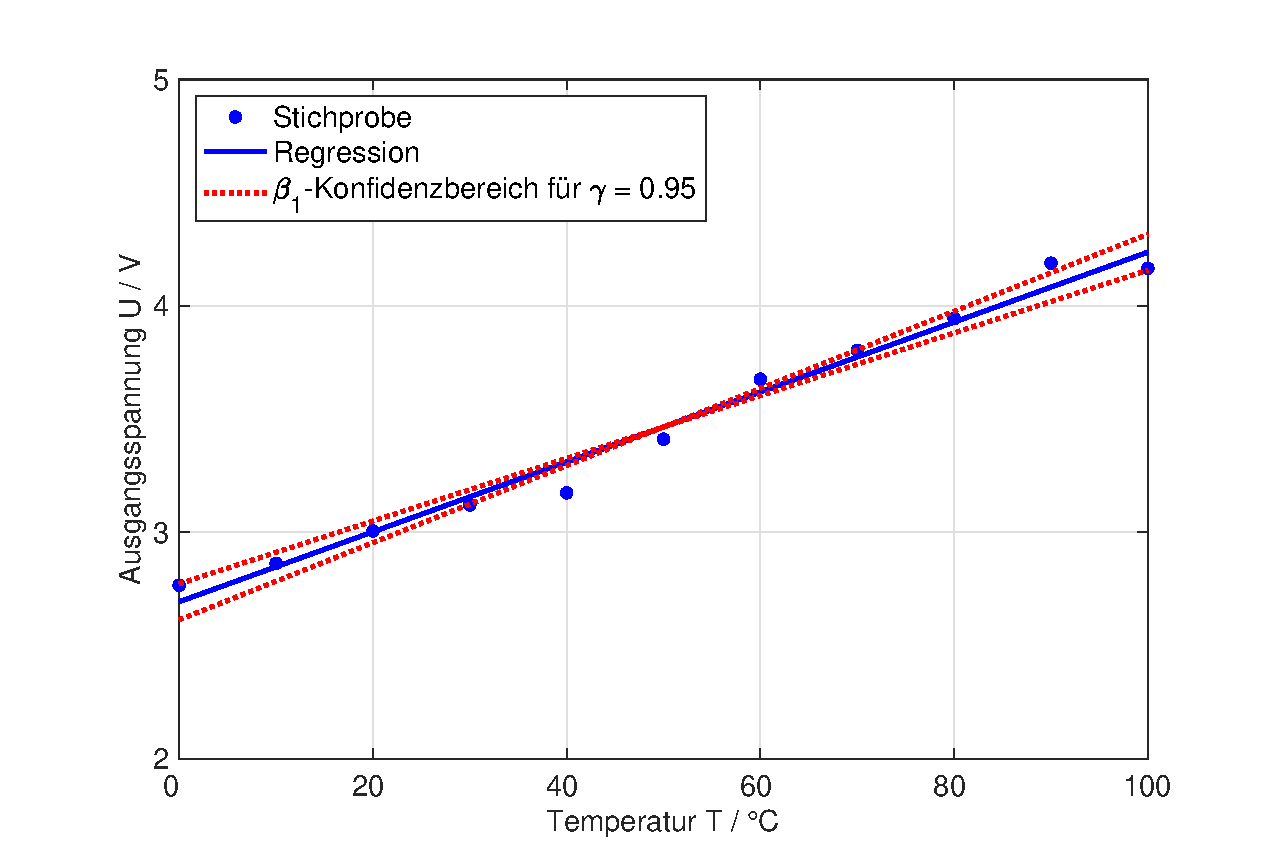
\includegraphics[width=0.5\textwidth]{Kapitel12/Bilder/image6}}
  \caption{Grafische Darstellung der Stichprobe f\"{u}r den Zusammenhang zwischen der \"{O}ltemperatur und der Ausgangsspannung eines Temperatursensors mit unterschiedlichen Regressionsgeraden}
  \label{fig:RegressionLinearOeltemperatur3}
\end{figure}

\fontfamily{phv}\selectfont
\noindent\textbf{Test des Regressionskoeffizienten $\beta_{1}$ auf Signifikanz}\smallskip

\noindent Zur Reduzierung der Komplexit\"{a}t von Regressionsfunktionen muss die Frage beantwortet werden, ob die berechneten Koeffizienten einen signifikanten Einfluss auf die Zielgr\"{o}{\ss}e besitzen. Es existieren verschiedene Verfahren zur Bewertung der Signifikanz von Regressionskoeffizienten, von denen zwei dargestellt werden sollen. Dies sind der t-Test und die Analyse des Konfidenzbereichs.\newline

\noindent Zur Bewertung der Signifikanz des Regressionskoeffizienten $\beta_{1}$ wird die Nullhypothese aufgestellt, dass der Korrelationskoeffizient $\beta_{1}$ einem Wert $\beta_{1}= 0$  entspricht. Trifft diese Hypothese zu, ist die Zielgr\"{o}{\ss}e y nicht von der Eingangsgr\"{o}{\ss}e x abh\"{a}ngig. Wird die Nullhypothese auf Basis der vorliegenden Stichprobe abgelehnt, kann davon ausgegangen werden, dass die Zielgr\"{o}{\ss}e y signifikant von dem Term $\beta_{1}\cdot c$ abh\"{a}ngt.\newline

\noindent Damit ein \"{u}ber die Stichprobe gesch\"{a}tzter Regressionskoeffizient $b_{1}$ mit einer spezifizierten Wahrscheinlichkeit zu der t-Verteilung aus Gleichung \eqref{eq:twelvethirtynine} geh\"{o}rt, muss dieser in dem Intervall $\beta_{1C1} < b_{1} \leq \beta_{1C2}$ liegen. Wird die Wahrscheinlichkeit daf\"{u}r mit $\gamma$ bezeichnet, gilt die Gleichung

\begin{equation}\label{eq:twelvefourtyeight}
P\left(\beta _{1C1} <b_{1} \le \beta _{1} {}_{C2} \right)=\gamma =1-\alpha
\end{equation}

\noindent Mit der Verteilung aus Gleichung \eqref{eq:twelvethirtynine} wird die Wahrscheinlichkeit $\gamma$, mit der die Variable t innerhalb des Intervalls $c_{1}$ {\dots} $c_{2}$ liegt, definiert als

\begin{equation}\label{eq:twelvefourtynine}
\gamma =P(c_{1} <t\le c_{2})=F(c_{2})-F(c_{1})
\end{equation}

\noindent Bei Annahme eines symmetrischen Tests ergeben sich die Konstanten $c_{1}$ und $c_{2}$ aus den Bedingungen

\begin{equation}\label{eq:twelvefifty}
F\left(c_{1} \right)=\dfrac{1-\gamma }{2} =\dfrac{\alpha }{2}
\end{equation}

\noindent und

\begin{equation}\label{eq:twelvefiftyone}
F(c_{2})=1-\dfrac{1-\gamma }{2} =1-\dfrac{\alpha }{2}
\end{equation}

\noindent Aufl\"{o}sen nach $c_{1}$ und $c_{2}$ f\"{u}hrt zu

\begin{equation}\label{eq:twelvefiftytwo}
c_{1} =F^{-1} \left(\dfrac{\alpha }{2} \right)
\end{equation}

\noindent und

\begin{equation}\label{eq:twelvefiftythree}
c_{2} =F^{-1} \left(1-\dfrac{\alpha }{2} \right)
\end{equation}

\noindent Durch Umformungen von Gleichung \eqref{eq:twelvethirtynine} und \eqref{eq:twelvefourtynine} ergibt sich ein Ausdruck f\"{u}r den Annahmebereich der Nullhypothese, n\"{a}mlich dass der gesch\"{a}tzte Regressionskoeffizient $b_{1}$ mit einer spezifizierten Wahrscheinlichkeit $\gamma$ zu der angenommenen t-Verteilung geh\"{o}rt. 

\begin{equation}\label{eq:twelvefiftyfour}
\gamma =P(c_{1} <t\le c_{2})=P\left(c_{1} \cdot s_{b1} <b_{1} \le c_{2} \cdot s_{b1} \right)
\end{equation}

\noindent Alternativ kann, wie in Kapitel 5 gezeigt wird, eine Unterschreitungswahrscheinlichkeit p der Pr\"{u}fgr\"{o}{\ss}e $b_{1}$ bestimmt werden und mit dem Signifikanzniveau $\alpha$ verglichen werden. Bei Hypothesentests mit beidseitigem Verwerfungsbereich $\beta_{1} \neq 0$  m\"{u}ssen f\"{u}r die Annahme der Nullhypothese die Bedingungen

\begin{equation}\label{eq:twelvefiftyfive}
p=P(t_{1})>\dfrac{\alpha }{2}
\end{equation}

\noindent und

\begin{equation}\label{eq:twelvefiftysix}
p=P(t_{1})\le 1-\dfrac{\alpha }{2}
\end{equation}

\noindent erf\"{u}llt werden. Damit l\"{a}sst sich der Test mit der Hypothese $\beta_{1} = 0$ und der Alternative $\beta_{1} \neq 0$  in folgenden Prozessschritten zusammenfassen.

\clearpage

\begin{table}[H]
\setlength{\arrayrulewidth}{.1em}
\caption{Test der Hypothese $\beta_{1} = 0$ gegen $\beta_{1} \neq 0$  f\"{u}r den Regressionskoeffizienten $\beta_{1}$ einer linearen Regression}
\setlength{\fboxsep}{0pt}%
\colorbox{lightgray}{%
\arrayrulecolor{white}%
\begin{tabular}{| wc{1cm} |wc{7.5cm} | wc{7.5cm}}
\xrowht{15pt}

\fontfamily{phv}\selectfont\textbf{Nr.} & 
\multicolumn{2}{c}{\fontfamily{phv}\selectfont\textbf{Prozessschritt}}\\ \hline \xrowht{20pt}

\fontfamily{phv}\selectfont{1} &
\multicolumn{2}{c}{\fontfamily{phv}\selectfont{Wahl eines Signifikanzniveaus  $\alpha$}} \\ \hline \xrowht{10pt}

\multirow{4}{*}{\fontfamily{phv}\selectfont{2}} &
\multicolumn{2}{c}{\fontfamily{phv}\selectfont{Bestimmung der zugehörigen Parameter $c_{1}$ und $c_{2}$ aus der inversen t-Verteilung mit}} \\ \xrowht{10pt}
&
\multicolumn{2}{c}{\fontfamily{phv}\selectfont{mit N - 2 Freiheitsgraden}} \\\xrowht{25pt}
& \multicolumn{2}{c}{\fontfamily{phv}\selectfont{$F(c_{1})=\dfrac{\alpha }{2}  \qquad \qquad \qquad  $ und $\qquad \quad \qquad F(c_{2})=1-\dfrac{\alpha }{2}$}}  \\ \hline \xrowht{20pt}

\multirow{4}{*}{\fontfamily{phv}\selectfont{3}} &
\multicolumn{2}{c}{\fontfamily{phv}\selectfont{Berechnung der Mittelwerte der Stichprobe}} \\\xrowht{25pt}
& \multicolumn{2}{c}{\fontfamily{phv}\selectfont{$\bar{x}=\dfrac{1}{N} \cdot \sum _{n=1}^{N}x_{n} \qquad \qquad \qquad \qquad $ und $\qquad  \qquad  \qquad \qquad \bar{y}=\dfrac{1}{N} \cdot \sum _{n=1}^{N}y_{n}$}}  \\ \hline \xrowht{20pt}

\multirow{4}{*}{\fontfamily{phv}\selectfont{4}} &
\multicolumn{2}{c}{\fontfamily{phv}\selectfont{Bestimmung der Standardabweichung und der Kovarianz der Stichprobe}} \\\xrowht{25pt}
& \multicolumn{2}{c}{\fontfamily{phv}\selectfont{$\qquad s_{x}=\sqrt{\dfrac{1}{N-1} \cdot \sum _{n=1}^{N}\left(x_{n} -\bar{x}\right)^{2}}\qquad\quad\; \qquad $ und $\qquad \qquad s_{xy} =\dfrac{1}{N-1} \cdot \left(\sum _{n=1}^{N}x_{n} \cdot y_{n} -N\cdot \bar{x}\cdot \bar{y}\right)$}}  \\ \hline \xrowht{20pt}

\multirow{4}{*}{\fontfamily{phv}\selectfont{5}} &
\multicolumn{2}{c}{\fontfamily{phv}\selectfont{Bestimmung der Parameter $b_{0}$ und $b_{1}$ der Regressionsgeraden}} \\\xrowht{30pt}
& \multicolumn{2}{c}{\fontfamily{phv}\selectfont{$b_{1} =\dfrac{\sum\limits _{n=1}^{N}x_{n} \cdot y_{n}  -N\cdot \bar{x}\cdot \bar{y}}{\sum\limits _{n=1}^{N}x_{n}^{2}  -N\cdot \bar{x}^{2} } =\dfrac{s_{xy} }{s_{x}^{2} }\qquad\qquad\;\; $ und $\qquad\qquad\qquad\qquad\qquad b_{0} =\bar{y}-b_{1} \cdot \bar{x}\qquad$}}  \\ \hline \xrowht{20pt}

\multirow{4}{*}{\fontfamily{phv}\selectfont{6}} &
\multicolumn{2}{c}{\fontfamily{phv}\selectfont{Berechnung der Fehlerquadratsumme}} \\\xrowht{35pt}
& \multicolumn{2}{c}{\fontfamily{phv}\selectfont{$a=\sum _{n=1}^{N}r_{n}^{2}  =\sum _{n=1}^{N}\left(y_{n} -b_{1} \cdot x_{n} -b_{0} \right)^{2} $}}  \\ \hline \xrowht{20pt}

\multirow{4}{*}{\fontfamily{phv}\selectfont{7}} &
\multicolumn{2}{c}{\fontfamily{phv}\selectfont{Bestimmung der Standardabweichung $s_{b1}$}} \\\xrowht{25pt}
& \multicolumn{2}{c}{\fontfamily{phv}\selectfont{$s_{b1} =\dfrac{\sqrt{a} }{\sqrt{N-1} \cdot \sqrt{N-2} \cdot s_{x}} $}}  \\ \hline \xrowht{15pt}

\multirow{4}{*}{\fontfamily{phv}\selectfont{8}} &
\multicolumn{2}{c}{\fontfamily{phv}\selectfont{Berechnung der Grenzen des Annahmebereiches}} \\\xrowht{25pt}
& \multicolumn{2}{c}{\fontfamily{phv}\selectfont{$\beta _{1C1} =c_{1} \cdot s_{b1}\qquad \qquad $ und $\qquad \qquad \beta _{1C2} =c_{2} \cdot s_{b1}$}} \\ \hline \xrowht{15pt}

\multirow{6}{*}{\fontfamily{phv}\selectfont{9}}  &
\multirow{2}{*}{\fontfamily{phv}\selectfont{Bestimmung des Annahmebereichs}} & \fontfamily{phv}\selectfont{Berechnung des p-Wertes mit der} \\
& & \fontfamily{phv}\selectfont{t-Verteilung mit N - 2 Freiheitsgraden} \\ \xrowht{40pt}
& \fontfamily{phv}\selectfont{$\beta _{1C1} <b_{1} \le \beta _{1C2}$} & 
\fontfamily{phv}\selectfont{$p=F\left(\dfrac{b_{1}}{s_{b1} } \right)$} \\ \hline\xrowht{15pt}

\multirow{4}{*}{\fontfamily{phv}\selectfont{10}}  &
\fontfamily{phv}\selectfont{F\"{u}r $\beta _{1C1} \leq b_{1}  < beta _{1C2}$ wird die Hypothese} & 
\fontfamily{phv}\selectfont{F\"{u}r $\alpha/2 \leq p < 1 - \alpha/2$ wird die Hypothese} \\ \xrowht{15pt}
& \fontfamily{phv}\selectfont{angenommen, f\"{u}r $b_{1} \leq \beta _{1C1}$ oder $b_{1} > \beta _{1C2}$} & \fontfamily{phv}\selectfont{angenommen, f\"{u}r $p < \alpha/2$ und $p \ge 1 -- \alpha/2$} \\ \xrowht{15pt}
&  \fontfamily{phv}\selectfont{wird die Hypothese verworfen} & \fontfamily{phv}\selectfont{wird die Hypothese verworfen} \\ \hline

\end{tabular}%
}\bigskip
\label{tab:twelvefour}
\end{table}

\clearpage

\noindent
\colorbox{lightgray}{%
\arrayrulecolor{white}%
\renewcommand\arraystretch{0.6}%
\begin{tabular}{ wl{16.5cm} }
{\fontfamily{phv}\selectfont
\noindent{Beispiel: Temperatursensor}}
\end{tabular}%
}\medskip 

\noindent F\"{u}r das Beispiel des Temperatursensors aus Tabelle \ref{tab:twelveone} wird die Nullhypothese $\beta_{1} = 0$ gegen die Alternativhypothese $\beta_{1} \neq 0$ getestet. Es liegen N = 11 Stichprobenwerte vor, sodass zur Bestimmung der Konstanten $c_{1}$ und $c_{2}$ eine t-Verteilung mit 9 Freiheitsgraden herangezogen wird. F\"{u}r ein Signifikanzniveau $\alpha = 0.05$ ergeben sich die Grenzen $c_{1}$ und $c_{2}$ zu

\begin{equation}\label{eq:twelvefiftyseven}
c_{1} =F^{-1} (1-0.975)=- 2.2622
\end{equation}

\noindent und

\begin{equation}\label{eq:twelvefiftyeight}
c_{2} =F^{-1} (1-0.025)= 2.2622
\end{equation}

\noindent Mit den obigen Angaben errechnet sich der Annahmebereich der Nullhypothese zu

\begin{equation}\label{eq:twelvefiftynine}
-0.0016 < b_{1} \le 0.0016
\end{equation}

\noindent Der gesch\"{a}tzte Wert des Regressionskoeffizienten liegt mit $b_{1}$ = 0.0154 au{\ss}erhalb dem in Gleichung \eqref{eq:twelvefiftynine} berechneten Annahmebereich. Die Nullhypothese wird somit auf Grundlage der vorliegenden Stichprobe verworfen, der Regressionskoeffizient $\beta_{1}$ ist ungleich 0 und damit signifikant.\newline

\noindent Alternativ kann zur Bewertung des Hypothesentests auch der p-Wert herangezogen werden. Dieser berechnet sich f\"{u}r die vorliegenden Hypothesen durch

\begin{equation}\label{eq:twelvesixty}
p=F\left(\dfrac{b_{1}}{s_{b1}} \right)
\end{equation}

\noindent Mit einem Wert von p = 1 liegt dieser deutlich \"{u}ber der Grenze von $1 - \alpha/2 = 0.975$. Die Nullhypothese muss daher verworfen werden, womit die Signifikanz des Regressionskoeffizienten $\beta_{1}$ best\"{a}tigt wird.\newline

\noindent Eine weitere M\"{o}glichkeit zur \"{U}berpr\"{u}fung der Signifikanz eines Regressionskoeffizienten ist dessen Konfidenzbereich. In Kapitel 6 wird gezeigt, dass wegen der linearen Abh\"{a}ngigkeit ein Hypothesentest in die Betrachtung eines Konfidenzbereichs \"{u}berf\"{u}hrt werden kann. Dadurch wird eine einfache Interpretation des Konfidenzbereichs zur Bewertung der Signifikanz erm\"{o}glicht: Schlie{\ss}t das Konfidenzintervall des Regressionskoeffizienten der Grundgesamtheit den entsprechenden Stichprobenwert ein, ist der untersuchte Koeffizient nicht signifikant. Andernfalls wird der Regressionskoeffizient als signifikant angenommen.\newline

\noindent F\"{u}r das Beispiel aus Tabelle 11.1 wurde der Konfidenzbereich des Regressionskoeffizienten $\beta_{1}$ bestimmt zu 

\begin{equation}\label{eq:twelvesixtyone}
0.0138 <\beta _{1} \le  0.0170
\end{equation}

\noindent Dieses Konfidenzintervall schlie{\ss}t die Zahl 0 nicht mit ein, sodass der Regressionskoeffizient auch nach diesem Kriterium als signifikant angenommen werden muss.

\clearpage

\subsubsection{Bewertung des Regressionskoeffizienten \texorpdfstring{$\beta_{0}$}{Lg}}

\noindent Die Vorgehensweise zur Berechnung der Verteilungsfunktion des Regressionskoeffizienten $\beta_{0}$ ist vergleichbar zu der des Regressionskoeffizienten $\beta_{1}$. Es wird die Zufallsvariable

\begin{equation}\label{eq:twelvesixtytwo}
z=\dfrac{b_{0} -\beta _{0} }{\sigma _{b_{0}}} =\dfrac{b_{0} -\beta _{0} }{\sqrt{\dfrac{\sum _{n=1}^{N}x_{n}^{2}  }{N\cdot (N-1)}} \cdot \dfrac{\sigma }{s_{x}}} =\dfrac{b_{0} -\beta _{0}}{\sigma } \cdot \dfrac{\sqrt{N} \cdot \sqrt{N-1} \cdot s_{x} }{\sqrt{\sum _{n=1}^{N}x_{n}^{2}}}
\end{equation}

\noindent aufgestellt. Mit den Vor\"{u}berlegungen in Abschnitt 11.1.1 weist sie eine Standard-Normalverteilung auf. Die Varianz $\sigma^{2}$ wird mit Gleichung \eqref{eq:twelvethirtyseven} gesch\"{a}tzt. Die Sch\"{a}tzung weist N - 2 Freiheitsgrade auf. Damit ist die Gr\"{o}{\ss}e 

\begin{equation}\label{eq:twelvesixtythree}
t=\dfrac{b_{0} -\beta _{0} }{\sqrt{a} \cdot \sqrt{\sum _{n=1}^{N}x_{n}^{2}  } } \cdot \sqrt{N} \cdot \sqrt{N-1} \cdot \sqrt{N-2} \cdot s_{x} =\dfrac{b_{0} -\beta _{0} }{s_{bo}}
\end{equation}

\noindent eine t-Verteilung mit N - 2 Freiheitsgraden auf, und die Standardabweichung s$_{b0}$ errechnet sich zu

\begin{equation}\label{eq:twelvesixtyfour}
s_{b0} =\dfrac{\sqrt{a} \cdot \sqrt{\sum _{n=1}^{N}x_{n}^{2}}}{\sqrt{N} \cdot \sqrt{N-1} \cdot \sqrt{N-2} \cdot s_{x}}
\end{equation}

{\fontfamily{phv}\selectfont
\noindent\textbf{Konfidenzintervall f\"{u}r den Regressionskoeffizienten $\beta_{0}$ }}\smallskip

\noindent Zur Berechnung des Konfidenzintervalls des Regressionskoeffizienten $\beta_{0}$ wird analog zum Regressionskoeffizienten $\beta_{1}$ die Zufallsvariable t verwendet. Der Konfidenzbereich berechnet sich dabei aus der Wahrscheinlichkeit

\begin{equation}\label{eq:twelvesixtyfive}
P(c_{1} <t\le c_{2})=F(c_{2})-F(c_{1})=\gamma
\end{equation}

\noindent Durch die Symmetrie des Konfidenzbereichs ergeben sich die Konstanten $c_{1}$ und $c_{2}$ zu

\begin{equation}\label{eq:twelvesixtysix}
c_{1} =F^{-1} \left(\dfrac{1-\gamma }{2} \right)
\end{equation}

\noindent und

\begin{equation}\label{eq:twelvesixtyseven}
c_{2} =F^{-1} \left(\dfrac{1+\gamma }{2} \right)
\end{equation}

\noindent Umformungen f\"{u}hren zu einem Ausdruck f\"{u}r den Konfidenzbereich des Regressionskoeffizienten $\beta_{0}$.

\begin{equation}\label{eq:twelvesixtyeight}
\gamma =P\left(c_{1} <t\le c_{2} \right)=P\left(c_{1} <\dfrac{b_{0} -\beta _{0} }{s_{b0} } \le c_{2} \right)=P\left(b_{0} -c_{2} \cdot s_{b0} \le \beta _{0} <b_{0} -c_{1} \cdot s_{b0} \right)
\end{equation}

\noindent Die Prozessschritte f\"{u}r das hier vorgestellte Vorgehen sind in Tabelle 11.3Tabelle 11.3 zusammengefasst.

\clearpage

\begin{table}[H]
\setlength{\arrayrulewidth}{.1em}
\caption{Vorgehen zur Bestimmung des Konfidenzbereichs f\"{u}r den Regressionskoeffizienten $\beta_{0}$}
\setlength{\fboxsep}{0pt}%
\colorbox{lightgray}{%
\arrayrulecolor{white}%
\begin{tabular}{| wc{1cm} | wc{15.5cm} }
\xrowht{15pt}

\fontfamily{phv}\selectfont\textbf{Nr.} & 
\fontfamily{phv}\selectfont\textbf{Prozessschritt}\\ \hline \xrowht{20pt}

\fontfamily{phv}\selectfont{1} &
\fontfamily{phv}\selectfont{Wahl einer Konfidenzzahl $\gamma$} \\ \hline \xrowht{10pt}

\multirow{4}{*}{\fontfamily{phv}\selectfont{2}} &
\fontfamily{phv}\selectfont{Bestimmung der zugehörigen Parameter $c_{1}$ und $c_{2}$ aus der inversen t-Verteilung} \\ \xrowht{10pt}
&
\fontfamily{phv}\selectfont{mit N - 2 Freiheitsgraden} \\\xrowht{25pt}
& \fontfamily{phv}\selectfont{$c_{1} =F^{-1} \left(\dfrac{1-\gamma }{2} \right)  \qquad \qquad \qquad  $ und $\qquad \quad \qquad c_{2} =F^{-1} \left(\dfrac{1-\gamma }{2} \right)$}  \\ \hline \xrowht{20pt}

\multirow{4}{*}{\fontfamily{phv}\selectfont{3}} &
\fontfamily{phv}\selectfont{Berechnung der Mittelwerte der Stichprobe} \\\xrowht{35pt}
& \fontfamily{phv}\selectfont{$\bar{x}=\dfrac{1}{N} \cdot \sum _{n=1}^{N}x_{n} \qquad \qquad \qquad \qquad $ und $\qquad  \qquad  \qquad \qquad \bar{y}=\dfrac{1}{N} \cdot \sum _{n=1}^{N}y_{n}$}  \\ \hline \xrowht{20pt}

\multirow{4}{*}{\fontfamily{phv}\selectfont{4}} &
\fontfamily{phv}\selectfont{Bestimmung der Standardabweichung und der Kovarianz der Stichprobe} \\\xrowht{35pt}
& \fontfamily{phv}\selectfont{$s_{x} =\sqrt{\dfrac{1}{N-1} \cdot \sum _{n=1}^{N}\left(x_{n} -\bar{x}\right)^{2}}\qquad \qquad $ und $\qquad \qquad s_{xy} =\dfrac{1}{N-1} \cdot \left(\sum _{n=1}^{N}x_{n} \cdot y_{n} -N\cdot \bar{x}\cdot \bar{y}\right)$}  \\ \hline \xrowht{20pt}

\multirow{5}{*}{\fontfamily{phv}\selectfont{5}} &
\fontfamily{phv}\selectfont{Bestimmung der Parameter $b_{0}$ und $b_{1}$ der Regressionsgeraden} \\\xrowht{40pt}
& \fontfamily{phv}\selectfont{$b_{1} =\dfrac{\sum\limits _{n=1}^{N}x_{n} \cdot y_{n}  -N\cdot \bar{x}\cdot \bar{y}}{\sum\limits _{n=1}^{N}x_{n}^{2}  -N\cdot \bar{x}^{2} } =\dfrac{s_{xy} }{s_{x}^{2} }\qquad \qquad $ und $\qquad \qquad b_{0} =\bar{y}-b_{1} \cdot \bar{x}$}  \\ \hline \xrowht{20pt}

\multirow{4}{*}{\fontfamily{phv}\selectfont{6}} &
\fontfamily{phv}\selectfont{Berechnung der Fehlerquadratsumme} \\\xrowht{35pt}
& \fontfamily{phv}\selectfont{$a=\sum _{n=1}^{N}r_{n}^{2}  =\sum _{n=1}^{N}\left(y_{n} -b_{1} \cdot x_{n} -b_{0} \right)^{2}  $}  \\ \hline \xrowht{20pt}

\multirow{4}{*}{\fontfamily{phv}\selectfont{7}} &
\fontfamily{phv}\selectfont{Bestimmung der Standardabweichung} \\\xrowht{30pt}
& \fontfamily{phv}\selectfont{$s_{b0} =\dfrac{\sqrt{a} \cdot \sqrt{\sum _{n=1}^{N}x_{n}^{2}}}{\sqrt{N} \cdot \sqrt{N-1} \cdot \sqrt{N-2} \cdot s_{x}}$}  \\ \hline \xrowht{20pt}

\multirow{4}{*}{\fontfamily{phv}\selectfont{8}} &
\fontfamily{phv}\selectfont{Bestimmung des  Konfidenzintervalls} \\\xrowht{25pt}
& \fontfamily{phv}\selectfont{$b_{0} -c_{2} \cdot s_{b0} \le \beta _{1} <b_{0} -c_{1} \cdot s_{b0} $}  \\ \hline

\end{tabular}%
}\bigskip
\label{tab:twelvefive}
\end{table}

\noindent
\colorbox{lightgray}{%
\arrayrulecolor{white}%
\renewcommand\arraystretch{0.6}%
\begin{tabular}{ wl{16.5cm} }
{\fontfamily{phv}\selectfont
\noindent{Beispiel: Temperatursensor}}
\end{tabular}%
}\medskip 

\noindent Die Vorgehensweise zur Berechnung des Konfidenzbereichs des Regressionskoeffizienten $\beta_{0}$ wird wieder an dem Beispiel des Temperatursensors aus Tabelle \ref{tab:twelveone} verdeutlicht. Es liegen wiederum N~=~11 Stichprobenwerte vor, sodass zur Bestimmung der Konstante $c_{1}$ und $c_{2}$ eine t-Verteilung mit 9 Freiheitsgraden herangezogen wird. F\"{u}r eine Konfidenzzahl von $\gamma = 0.95$ ergeben sich die Grenze $c_{1}$ und $c_{2}$ zu

\begin{equation}\label{eq:twelvesixtynine}
c_{1} =F^{-1} (1-0.975)=-2.2622
\end{equation}

\noindent und 

\begin{equation}\label{eq:twelveseventy}
c_{2} =F^{-1} (1-0.025)=2.2622
\end{equation}

\noindent Mit den Angaben errechnet sich der Konfidenzbereich des Regressionskoeffizienten $\beta_{0}$ mit dem gesch\"{a}tzten Regressionsparameter $b_{0} = 2.6930$ und der Standardabweichung $s_{x} = 33.1662$ zu

\begin{equation}\label{eq:twelveseventyone}
2.5988 \le \beta _{0} <  2.7873
\end{equation}

\noindent In das Temperatur-Spannungs-Diagramm in Bild 11.6 wurde neben den Messwerten und der gesch\"{a}tzten Regressionsgeraden mit dem Regressionskoeffizienten $b_{0}$ noch zwei weitere Gerade eingezeichnet. Diese ergeben sich durch die Extremwerte des 95\% - Konfidenzintervalls.

\noindent 
\begin{figure}[H]
  \centerline{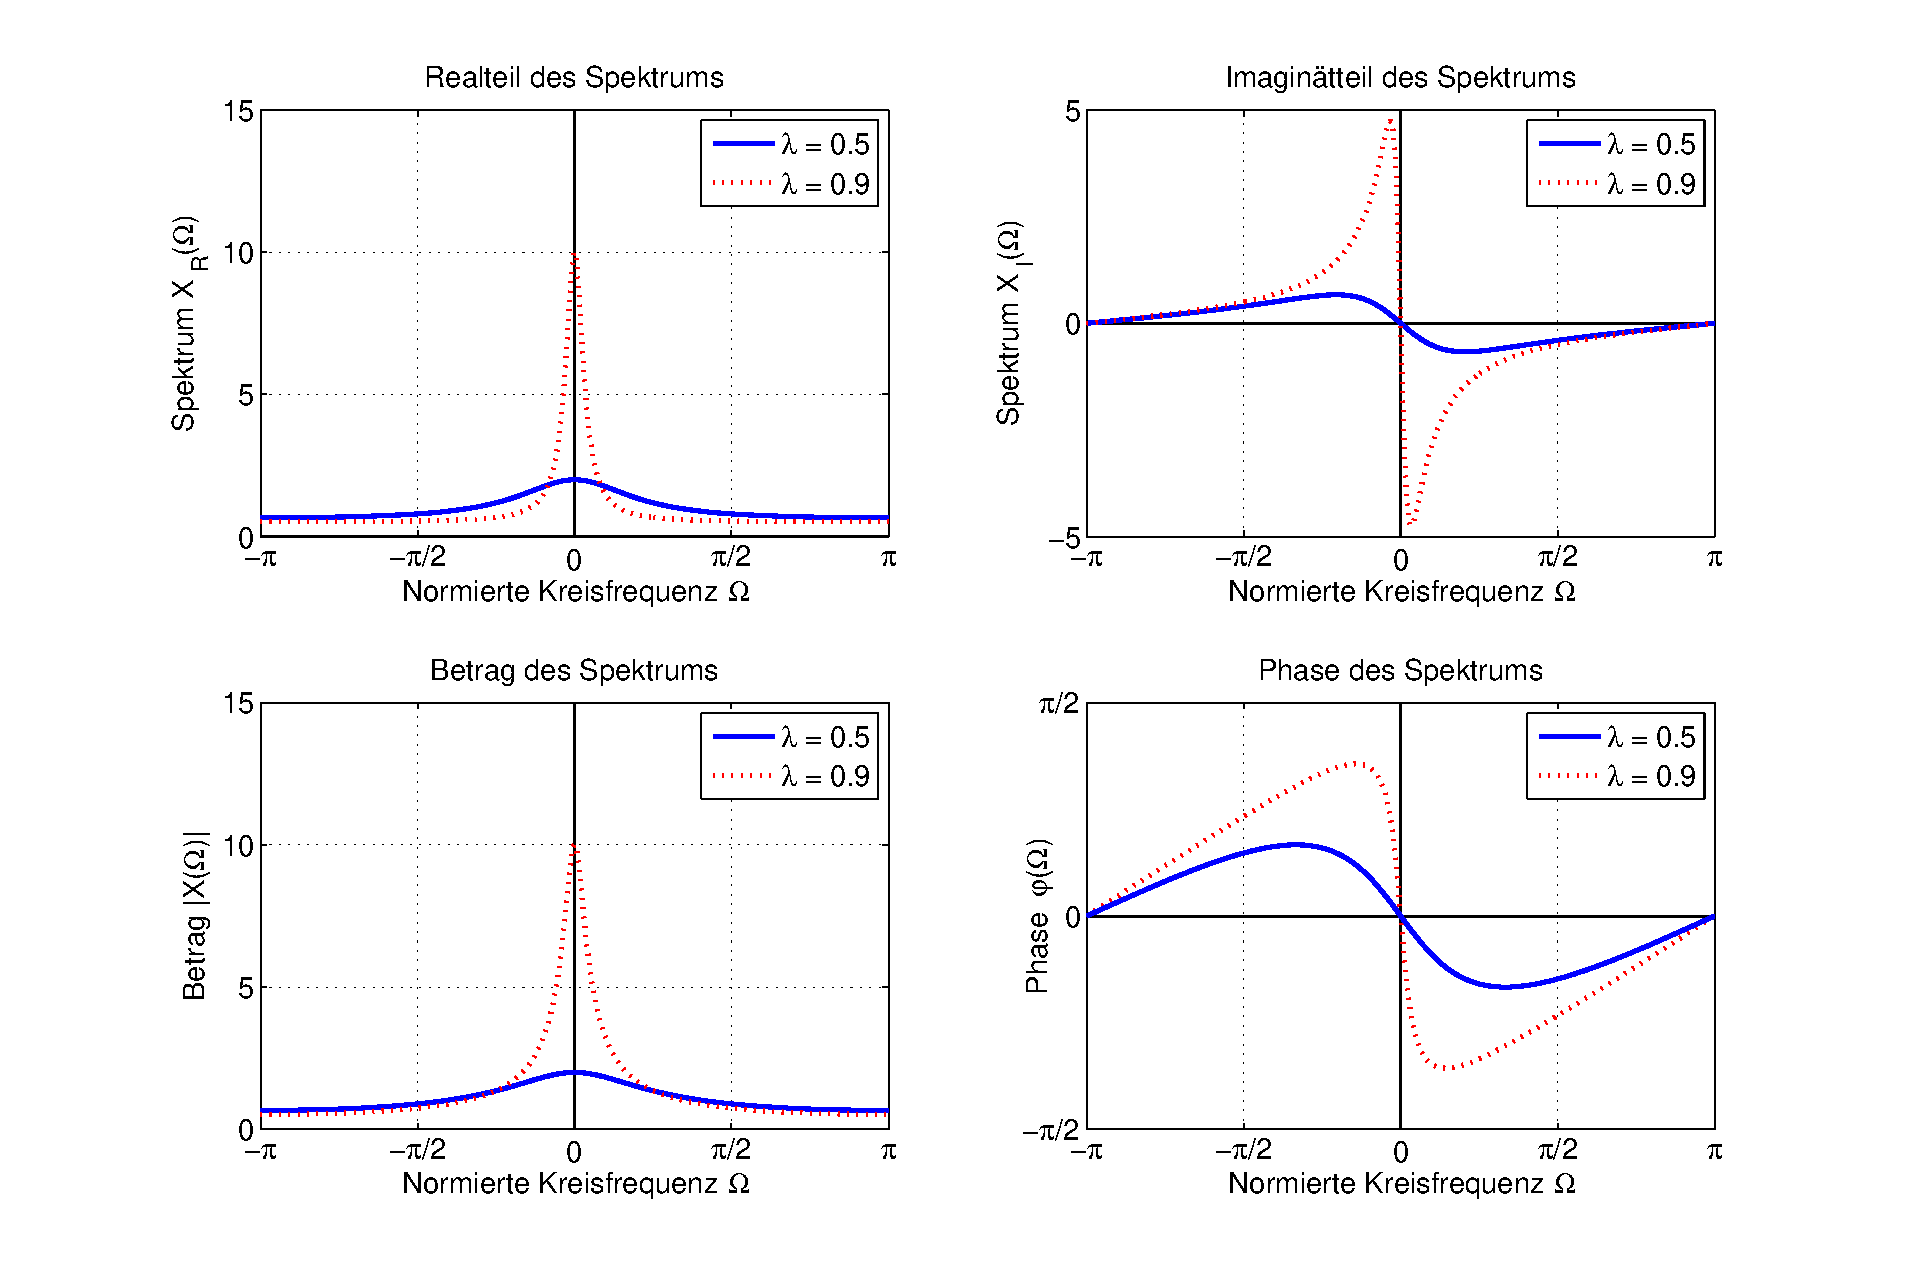
\includegraphics[width=0.5\textwidth]{Kapitel12/Bilder/image7}}
  \caption{Grafische Darstellung der Stichprobe f\"{u}r den Zusammenhang zwischen \"{O}ltemperatur und Ausgangsspannung eines Temperatursensors mit unterschiedlichen Regressionsgeraden}
  \label{fig:RegressionLinearOeltemperatur4}
\end{figure}

\fontfamily{phv}\selectfont
\noindent\textbf{Test des Regressionskoeffizienten $\beta_{0}$ auf Signifikanz}\smallskip

\noindent Zur Bewertung der Signifikanz des Regressionskoeffizienten $\beta_{0}$ wird die Nullhypothese gepr\"{u}ft, dass der Korrelationskoeffizient $\beta_{0}$ einem Wert $\beta_{0}$ = 0 entspricht. Trifft diese Hypothese zu, liegt bei dem untersuchten System kein Gleichanteil vor. Wird die Nullhypothese auf Basis der vorliegenden Stichprobe abgelehnt, kann davon ausgegangen werden, dass das untersuchte System einen Gleichanteil besitzt.\newline

\noindent Damit ein \"{u}ber die Stichprobe gesch\"{a}tzter Regressionskoeffizient $b_{0}$ mit einer spezifizierten Wahrscheinlichkeit zu der t-Verteilung aus Gleichung \eqref{eq:twelvesixtythree} geh\"{o}rt, muss dieser in dem Intervall $\beta_{0C1} < b_{0} \leq \beta_{0C2}$ liegen. Wird die Wahrscheinlichkeit daf\"{u}r mit $\gamma$ bezeichnet, gilt die Gleichung

\begin{equation}\label{eq:twelveseventytwo}
P\left(\beta _{0C1} <b_{0} \le \beta _{0C2} \right)=\gamma =1-\alpha
\end{equation}

\noindent Mit der Verteilung aus Gleichung \eqref{eq:twelvesixtythree} wird nach Gleichung \eqref{eq:twelveseventytwo} die Wahrscheinlichkeit $\gamma$, mit der die Variable t innerhalb des Intervalls $c_{1}$ {\dots} $c_{2}$ liegt, definiert als

\begin{equation}\label{eq:twelveseventythree}
\gamma =P(c_{1} <t\le c_{2})=F(c_{2})-F(c_{1})
\end{equation}

\noindent Bei Annahme eines symmetrischen Tests ergeben sich die Konstanten $c_{1}$ und $c_{2}$ aus den Bedingungen

\begin{equation}\label{eq:twelveseventyfour}
c_{1} =F^{-1} \left(\dfrac{\alpha }{2} \right)
\end{equation}

\noindent und

\begin{equation}\label{eq:twelveseventyfive}
c_{2} =F^{-1} \left(1-\dfrac{\alpha }{2} \right)
\end{equation}

\noindent Durch Umformungen von Gleichung \eqref{eq:twelvesixtythree} und \eqref{eq:twelveseventythree} ergibt sich ein Ausdruck f\"{u}r den Annahmebereich der Nullhypothese, n\"{a}mlich dass der gesch\"{a}tzte Regressionskoeffizient $b_{0}$ mit einer spezifizierten Wahrscheinlichkeit $\gamma$ zu der angenommenen t-Verteilung geh\"{o}rt.

\begin{equation}\label{eq:twelveseventysix}
\gamma =P(c_{1} <t\le c_{2})=P(c_{1} \cdot s_{b0} <b_{0} \le c_{2} \cdot s_{b0})
\end{equation}

\noindent Alternativ kann, wie in Kapitel \ref{six} gezeigt wird, eine Unterschreitungswahrscheinlichkeit p der Pr\"{u}fgr\"{o}{\ss}e $b_{0}$ bestimmt werden und mit dem Signifikanzniveau $\alpha$ verglichen werden. Bei Hypothesentests mit beidseitigem Verwerfungsbereich $\beta_{0} \neq 0$  m\"{u}ssen f\"{u}r die Annahme der Nullhypothese die Bedingungen

\begin{equation}\label{eq:twelveseventyseven}
p=F(t)>\dfrac{\alpha }{2}
\end{equation}

\noindent und

\begin{equation}\label{eq:twelveseventyeight}
p=F(t)>\dfrac{\alpha }{2}
\end{equation}

\noindent erf\"{u}llt werden. Damit l\"{a}sst sich der Test mit der Hypothese $\beta_{0} = 0$ und der Alternative $\beta_{0} \neq 0$ in folgenden Prozessschritten zusammenfassen.

\clearpage

\begin{table}[H]
\setlength{\arrayrulewidth}{.1em}
\caption{Test der Hypothese $\beta_{0} = 0$ gegen $\beta_{0} \neq 0$  f\"{u}r den Regressionskoeffizienten $\beta_{0}$ einer linearen Regression}
\setlength{\fboxsep}{0pt}%
\colorbox{lightgray}{%
\arrayrulecolor{white}%
\begin{tabular}{| wc{1cm} |wc{7.5cm} | wc{7.5cm}}
\xrowht{15pt}

\fontfamily{phv}\selectfont\textbf{Nr.} & 
\multicolumn{2}{c}{\fontfamily{phv}\selectfont\textbf{Prozessschritt}}\\ \hline \xrowht{20pt}

\fontfamily{phv}\selectfont{1} &
\multicolumn{2}{c}{\fontfamily{phv}\selectfont{Wahl eines Signifikanzniveaus  $\alpha$}} \\ \hline \xrowht{10pt}

\multirow{4}{*}{\fontfamily{phv}\selectfont{2}} &
\multicolumn{2}{c}{\fontfamily{phv}\selectfont{Bestimmung der zugehörigen Parameter $c_{1}$ und $c_{2}$ aus der inversen t-Verteilung mit}} \\ \xrowht{10pt}
&
\multicolumn{2}{c}{\fontfamily{phv}\selectfont{mit N - 2 Freiheitsgraden}} \\\xrowht{25pt}
& \multicolumn{2}{c}{\fontfamily{phv}\selectfont{$c_{1} =F^{-1} (\dfrac{\alpha }{2})  \qquad \qquad \qquad  $ und $\qquad \quad \qquad c_{2} =F^{-1} (1-\dfrac{\alpha }{2} )$}}  \\ \hline \xrowht{20pt}

\multirow{4}{*}{\fontfamily{phv}\selectfont{3}} &
\multicolumn{2}{c}{\fontfamily{phv}\selectfont{Berechnung der Mittelwerte der Stichprobe}} \\\xrowht{25pt}
& \multicolumn{2}{c}{\fontfamily{phv}\selectfont{$\bar{x}=\dfrac{1}{N} \cdot \sum _{n=1}^{N}x_{n} \qquad \qquad \qquad \qquad $ und $\qquad  \qquad  \qquad \qquad \bar{y}=\dfrac{1}{N} \cdot \sum _{n=1}^{N}y_{n}$}}  \\ \hline \xrowht{20pt}

\multirow{4}{*}{\fontfamily{phv}\selectfont{4}} &
\multicolumn{2}{c}{\fontfamily{phv}\selectfont{Bestimmung der Standardabweichung und der Kovarianz der Stichprobe}} \\\xrowht{25pt}
& \multicolumn{2}{c}{\fontfamily{phv}\selectfont{$\qquad s_{x}=\sqrt{\dfrac{1}{N-1} \cdot \sum _{n=1}^{N}\left(x_{n} -\bar{x}\right)^{2}}\qquad\quad\; \qquad $ und $\qquad \qquad s_{xy} =\dfrac{1}{N-1} \cdot \left(\sum _{n=1}^{N}x_{n} \cdot y_{n} -N\cdot \bar{x}\cdot \bar{y}\right)$}}  \\ \hline \xrowht{20pt}

\multirow{4}{*}{\fontfamily{phv}\selectfont{5}} &
\multicolumn{2}{c}{\fontfamily{phv}\selectfont{Bestimmung der Parameter $b_{0}$ und $b_{1}$ der Regressionsgeraden}} \\\xrowht{30pt}
& \multicolumn{2}{c}{\fontfamily{phv}\selectfont{$b_{1} =\dfrac{\sum\limits _{n=1}^{N}x_{n} \cdot y_{n}  -N\cdot \bar{x}\cdot \bar{y}}{\sum\limits _{n=1}^{N}x_{n}^{2}  -N\cdot \bar{x}^{2} } =\dfrac{s_{xy} }{s_{x}^{2} }\qquad\qquad\;\; $ und $\qquad\qquad\qquad\qquad\qquad b_{0} =\bar{y}-b_{1} \cdot \bar{x}\qquad$}}  \\ \hline \xrowht{20pt}

\multirow{4}{*}{\fontfamily{phv}\selectfont{6}} &
\multicolumn{2}{c}{\fontfamily{phv}\selectfont{Berechnung der Fehlerquadratsumme}} \\\xrowht{35pt}
& \multicolumn{2}{c}{\fontfamily{phv}\selectfont{$a=\sum _{n=1}^{N}r_{n}^{2}  =\sum _{n=1}^{N}\left(y_{n} -b_{1} \cdot x_{n} -b_{0} \right)^{2} $}}  \\ \hline \xrowht{20pt}

\multirow{4}{*}{\fontfamily{phv}\selectfont{7}} &
\multicolumn{2}{c}{\fontfamily{phv}\selectfont{Bestimmung der Standardabweichung $s_{b1}$}} \\\xrowht{25pt}
& \multicolumn{2}{c}{\fontfamily{phv}\selectfont{$s_{b0} =\dfrac{\sqrt{a} \cdot \sqrt{\sum _{n=1}^{N}x_{n}^{2}} }{\sqrt{N} \cdot \sqrt{N-1} \cdot \sqrt{N-2} \cdot s_{x}} $}}  \\ \hline \xrowht{15pt}

\multirow{4}{*}{\fontfamily{phv}\selectfont{8}} &
\multicolumn{2}{c}{\fontfamily{phv}\selectfont{Berechnung der Grenzen des Annahmebereiches}} \\\xrowht{25pt}
& \multicolumn{2}{c}{\fontfamily{phv}\selectfont{$\beta _{0C1} =c_{1} \cdot s_{b0}\qquad \qquad $ und $\qquad \qquad \beta _{0C2} =c_{2} \cdot s_{b0}$}} \\ \hline \xrowht{15pt}

\multirow{6}{*}{\fontfamily{phv}\selectfont{9}}  &
\multirow{2}{*}{\fontfamily{phv}\selectfont{Bestimmung des Annahmebereichs}} & \fontfamily{phv}\selectfont{Berechnung des p-Wertes mit der} \\
& & \fontfamily{phv}\selectfont{t-Verteilung mit N - 2 Freiheitsgraden} \\ \xrowht{40pt}
& \fontfamily{phv}\selectfont{$\beta _{0C1} <b_{1} \le \beta _{0C2}$} & 
\fontfamily{phv}\selectfont{$p=F\left(\dfrac{b_{0}}{s_{b0} } \right)$} \\ \hline\xrowht{15pt}

\multirow{4}{*}{\fontfamily{phv}\selectfont{10}}  &
\fontfamily{phv}\selectfont{F\"{u}r $\beta _{0C1} \leq b_{0}  < \beta _{0C2}$ wird die Hypothese} & 
\fontfamily{phv}\selectfont{F\"{u}r $\alpha/2 \leq p < 1 - \alpha/2$ wird die Hypothese} \\ \xrowht{15pt}
& \fontfamily{phv}\selectfont{angenommen, f\"{u}r $b_{0} \leq \beta _{0C1}$ oder $b_{0} > \beta _{0C2}$} & \fontfamily{phv}\selectfont{angenommen, f\"{u}r $p < \alpha/2$ und $p \ge 1 -- \alpha/2$} \\ \xrowht{15pt}
&  \fontfamily{phv}\selectfont{wird die Hypothese verworfen} & \fontfamily{phv}\selectfont{wird die Hypothese verworfen} \\ \hline

\end{tabular}%
}\bigskip
\label{tab:twelvesix}
\end{table}

\clearpage

\noindent
\colorbox{lightgray}{%
\arrayrulecolor{white}%
\renewcommand\arraystretch{0.6}%
\begin{tabular}{ wl{16.5cm} }
{\fontfamily{phv}\selectfont
\noindent{Beispiel: Temperatursensor}}
\end{tabular}%
}\medskip 

\noindent F\"{u}r das Beispiel des Temperatursensors aus Tabelle 11.1 wird die Nullhypothese $\beta_{0} = 0$ gegen die Alternativhypothese $\beta_{0} \neq 0$ getestet. Es liegen N = 11 Stichprobenwerte vor, sodass zur Bestimmung der Konstanten $c_{1}$ und $c_{2}$ eine t-Verteilung mit 9 Freiheitsgraden herangezogen wird. F\"{u}r ein Signifikanzniveau $\alpha$ = 0.05 ergeben sich die Grenzen $c_{1}$ und $c_{2}$ zu

\begin{equation}\label{eq:twelveseventynine}
c_{1} =F^{-1} (1-0.975)=- 2.2622
\end{equation}

\noindent und

\begin{equation}\label{eq:twelveeighty}
c_{2} =F^{-1} (1-0.025)= 2.2622
\end{equation}

\noindent Mit den Angaben errechnet sich der Annahmebereich der Nullhypothese zu

\begin{equation}\label{eq:twelveeightyone}
-0.0943 <b_{0} \le 0.0943
\end{equation}

\noindent Der gesch\"{a}tzte Wert des Regressionskoeffizienten liegt mit $b_{0}$ = 2.6930 au{\ss}erhalb des in Gleichung \eqref{eq:twelvefiftynine} berechneten Annahmebereich. Die Nullhypothese wird somit auf Grundlage der vorliegenden Stichprobe verworfen, der Regressionskoeffizient $\beta_{0}$ ist ungleich 0 und damit signifikant.\newline

\noindent Alternativ kann zur Bewertung des Hypothesentests auch der p-Wert herangezogen werden. Dieser berechnet sich f\"{u}r die vorliegenden Hypothesen durch

\begin{equation}\label{eq:twelveeightytwo}
p=F\left(\dfrac{b_{0}}{s_{b0}} \right)
\end{equation}

\noindent Der Wert p = 1 liegt deutlich \"{u}ber der Grenze von $1 - \alpha/2 = 0.975$. Die Nullhypothese muss daher verworfen werden, womit die Signifikanz des Regressionskoeffizienten $\beta_{0}$ aufgezeigt wird.\newline

\noindent Eine weitere M\"{o}glichkeit zur \"{U}berpr\"{u}fung der Signifikanz eines Regressionskoeffizienten ist dessen Konfidenzbereich. F\"{u}r das Beispiel aus Tabelle 11.1 wurde der Konfidenzbereich des Regressionskoeffizienten $\beta_{0}$ bestimmt zu 

\begin{equation}\label{eq:twelveeightythree}
2.5988 \le \beta _{0} <  2.7873
\end{equation}

\noindent Dieses Konfidenzintervall schlie{\ss}t die Zahl 0 nicht mit ein, sodass der Regressionskoeffizient auch nach diesem Kriterium als signifikant angenommen werden muss.

\clearpage

\subsubsection{Konfidenzintervall f\"{u}r den Erwartungswert}

\noindent Mit der Regressionsgleichung wird die Zielgr\"{o}{\ss}e $y_{0}$ als Funktion der festen Eingangsgr\"{o}{\ss}en $x_{0}$ gesch\"{a}tzt. 

\begin{equation}\label{eq:twelveeightyfour}
y(x_{0})=b_{0} +b_{1} \cdot x_{0}
\end{equation}

\noindent Dabei werden $b_{0}$ und $b_{1}$ auf Basis des vorliegenden Datensatzes gesch\"{a}tzt, sie sind damit selber Zufallsvariablen. F\"{u}r den Erwartungswert gilt:

\begin{equation}\label{eq:twelveeightyfive}
\mu _{y} (x_{0})=E(y_{0})=E(b_{0} +b_{1} \cdot x_{0})=E(b_{0})+E(b_{1} \cdot x_{0})=\beta _{0} +\beta _{1} \cdot x_{0}
\end{equation}

\noindent Die Regression ist erwartungstreu, weil die Regressionskoeffizienten $\beta_{0}$ und $\beta_{1}$ erwartungstreu gesch\"{a}tzt werden. Bei der Berechnung des Konfidenzintervalls f\"{u}r den Erwartungswert $\mu_{y}(x_{0})$ wird eine Variable ben\"{o}tigt, deren Verteilung bekannt ist und in der der Erwartungswert sowie der gesch\"{a}tzte Wert $y(x_{0}$) vorkommt. Der Sch\"{a}tzwert berechnet sich zu

\begin{equation}\label{eq:twelveeightysix}
y(x_{0})=b_{1} \cdot x_{0} +b_{0} =b_{1} \cdot (x_{0} -\bar{x})+\bar{y}
\end{equation}

\noindent Damit ist die Gr\"{o}{\ss}e 

\begin{equation}\label{eq:twelveeightyseven}
z=\dfrac{y\left(x_{0} \right)-\mu _{y} (x_{0})}{\sigma _{y0}} =\dfrac{b_{1} \cdot \left(x_{0} -\bar{x}\right)+\bar{y}-\mu _{y} \left(x_{0} \right)}{\sqrt{\sigma _{b_{1}}^{2} \cdot \left(x_{0} -\bar{x}\right)^{2} +\sigma _{\bar{y}}^{2}}} =\dfrac{b_{1} \cdot (x_{0} -\bar{x})+\bar{y}-\mu _{y} (x_{0})}{\sigma \cdot \sqrt{\dfrac{(x_{0} -\bar{x})^{2} }{(N-1)\cdot s_{x}^{2} } +\dfrac{1}{N}}}
\end{equation}

\noindent standard-normalverteilt. Die Varianz $\sigma^{2}$ wird mit Gleichung \eqref{eq:twelvethirtyseven} gesch\"{a}tzt. Die Sch\"{a}tzung weist N - 2 Freiheitsgrade auf. Damit besitzt die Gr\"{o}{\ss}e 

\begin{equation}\label{eq:twelveeightyeight}
t=\dfrac{b_{1} \cdot (x_{0} -\bar{x})+\bar{y}-\mu _{y} (x_{0})}{\sqrt{\dfrac{(x_{0} -\bar{x})^{2}}{(N-1)\cdot s_{x}^{2}} +\dfrac{1}{N}} \cdot \sqrt{\dfrac{a}{N-2}}} =\dfrac{y(x_{0})-\mu _{y} (x_{0})}{s_{y0}}
\end{equation}

\noindent eine t-Verteilung mit N - 2 Freiheitsgraden auf, und die Standardabweichung $s_{y0}$ errechnet sich zu

\begin{equation}\label{eq:twelveeightynine}
s_{y0} =\sqrt{\dfrac{(x_{0} -\bar{x})^{2}}{(N-1)\cdot s_{x}^{2}} +\dfrac{1}{N}} \cdot \sqrt{\dfrac{a}{N-2}}
\end{equation}

\noindent Die Zufallsvariable t wird zur Bestimmung des Konfidenzbereichs f\"{u}r den Erwartungswert $\mu_{y}(x_{0})$ verwendet. Er berechnet sich aus der Wahrscheinlichkeit

\begin{equation}\label{eq:twelveninety}
P(c_{1} <t\le c_{2})=F(c_{2})-F(c_{1})=\gamma
\end{equation}

\noindent Durch die Symmetrie des Konfidenzbereichs ergeben sich die Konstanten $c_{1}$ und $c_{2}$ zu

\begin{equation}\label{eq:twelveninetyone}
c_{1} =F^{-1} \left(\dfrac{1-\gamma }{2} \right)
\end{equation}

\noindent und

\begin{equation}\label{eq:twelveninetytwo}
c_{2} =F^{-1} \left(\dfrac{1-\gamma }{2} \right)
\end{equation}

\noindent Durch Umformungen ergibt sich ein Ausdruck f\"{u}r den Konfidenzbereich des Mittelwertes.

\begin{equation}\label{eq:twelveninetythree}
\gamma =P(c_{1} <t\le c_{2})=P\left(y(x_{0})-c_{2} \cdot s_{y0} \le \mu _{y} (x_{0})<y(x_{0})-c_{1} \cdot s_{y0} \right)
\end{equation}

\noindent Das Verfahren wird in Tabelle \ref{tab:twelveseven} beschrieben.

\begin{table}[H]
\setlength{\arrayrulewidth}{.1em}
\caption{Vorgehen zur Bestimmung des Konfidenzbereichs f\"{u}r den Mittelwert einer Regressionsgerade}
\setlength{\fboxsep}{0pt}%
\colorbox{lightgray}{%
\arrayrulecolor{white}%
\begin{tabular}{| wc{1cm} | wc{15.5cm} }
\xrowht{15pt}

\fontfamily{phv}\selectfont\textbf{Nr.} & 
\fontfamily{phv}\selectfont\textbf{Prozessschritt}\\ \hline \xrowht{20pt}

\fontfamily{phv}\selectfont{1} &
\fontfamily{phv}\selectfont{Wahl einer Konfidenzzahl $\gamma$} \\ \hline \xrowht{10pt}

\multirow{4}{*}{\fontfamily{phv}\selectfont{2}} &
\fontfamily{phv}\selectfont{Bestimmung der zugehörigen Parameter $c_{1}$ und $c_{2}$ aus der inversen t-Verteilung} \\ \xrowht{10pt}
&
\fontfamily{phv}\selectfont{mit N - 2 Freiheitsgraden} \\\xrowht{25pt}
& \fontfamily{phv}\selectfont{$c_{1} =F^{-1} \left(\dfrac{1-\gamma }{2} \right)  \qquad \qquad \qquad  $ und $\qquad \quad \qquad c_{2} =F^{-1} \left(\dfrac{1-\gamma }{2} \right)$}  \\ \hline \xrowht{20pt}

\multirow{4}{*}{\fontfamily{phv}\selectfont{3}} &
\fontfamily{phv}\selectfont{Berechnung der Mittelwerte der Stichprobe} \\\xrowht{35pt}
& \fontfamily{phv}\selectfont{$\bar{x}=\dfrac{1}{N} \cdot \sum _{n=1}^{N}x_{n} \qquad \qquad \qquad \qquad $ und $\qquad  \qquad  \qquad \qquad \bar{y}=\dfrac{1}{N} \cdot \sum _{n=1}^{N}y_{n}$}  \\ \hline \xrowht{20pt}

\multirow{4}{*}{\fontfamily{phv}\selectfont{4}} &
\fontfamily{phv}\selectfont{Bestimmung der Standardabweichung und der Kovarianz der Stichprobe} \\\xrowht{35pt}
& \fontfamily{phv}\selectfont{$s_{x} =\sqrt{\dfrac{1}{N-1} \cdot \sum _{n=1}^{N}\left(x_{n} -\bar{x}\right)^{2}}\qquad \qquad $ und $\qquad \qquad s_{xy} =\dfrac{1}{N-1} \cdot \left(\sum _{n=1}^{N}x_{n} \cdot y_{n} -N\cdot \bar{x}\cdot \bar{y}\right)$}  \\ \hline \xrowht{20pt}

\multirow{5}{*}{\fontfamily{phv}\selectfont{5}} &
\fontfamily{phv}\selectfont{Bestimmung der Parameter $b_{0}$ und $b_{1}$ der Regressionsgeraden} \\\xrowht{40pt}
& \fontfamily{phv}\selectfont{$b_{1} =\dfrac{\sum\limits _{n=1}^{N}x_{n} \cdot y_{n}  -N\cdot \bar{x}\cdot \bar{y}}{\sum\limits _{n=1}^{N}x_{n}^{2}  -N\cdot \bar{x}^{2} } =\dfrac{s_{xy} }{s_{x}^{2} }\qquad \qquad $ und $\qquad \qquad b_{0} =\bar{y}-b_{1} \cdot \bar{x}$}  \\ \hline \xrowht{20pt}

\multirow{4}{*}{\fontfamily{phv}\selectfont{6}} &
\fontfamily{phv}\selectfont{Berechnung der Fehlerquadratsumme} \\\xrowht{35pt}
& \fontfamily{phv}\selectfont{$a=\sum _{n=1}^{N}r_{n}^{2}  =\sum _{n=1}^{N}\left(y_{n} -b_{1} \cdot x_{n} -b_{0} \right)^{2}  $}  \\ \hline \xrowht{20pt}

\multirow{4}{*}{\fontfamily{phv}\selectfont{7}} &
\fontfamily{phv}\selectfont{Bestimmung der Standardabweichung $s_{y0}$} \\\xrowht{30pt}
& \fontfamily{phv}\selectfont{$s_{y0} =\sqrt{\dfrac{(x_{0} -\bar{x})^{2}}{(N-1)\cdot s_{x}^{2}} +\dfrac{1}{N}} \cdot \sqrt{\dfrac{a}{N-2}}$}  \\ \hline \xrowht{20pt}

\multirow{4}{*}{\fontfamily{phv}\selectfont{8}} &
\fontfamily{phv}\selectfont{Bestimmung des  Konfidenzintervalls} \\\xrowht{25pt}
& \fontfamily{phv}\selectfont{$y(x_{0})-c_{2} \cdot s_{y0} \le \mu _{y} (x_{0})<y(x_{0})-c_{1} \cdot s_{y0}$}  \\ \hline

\end{tabular}%
}\bigskip
\label{tab:twelveseven}
\end{table}

\clearpage

\noindent Der Konfidenzbereich des Mittelwertes ist von der Zufallsvariablen x abh\"{a}ngig und erreicht seine minimale L\"{a}nge an der Stelle $x = \bar{x}$. Mit steigendem Abstand x von dem Mittelwert steigt die L\"{a}nge des Konvergenzintervalls an. \bigskip

\noindent
\colorbox{lightgray}{%
\arrayrulecolor{white}%
\renewcommand\arraystretch{0.6}%
\begin{tabular}{ wl{16.5cm} }
{\fontfamily{phv}\selectfont
\noindent{Beispiel: Temperatursensor}}
\end{tabular}%
}\medskip 

\noindent Bild \ref{fig:RegressionLinearOeltemperatur5} zeigt den Konvergenzbereich f\"{u}r das Beispiel des \"{O}ltemperatursensors aus Tabelle \ref{tab:twelveone}.

\noindent 
\begin{figure}[H]
  \centerline{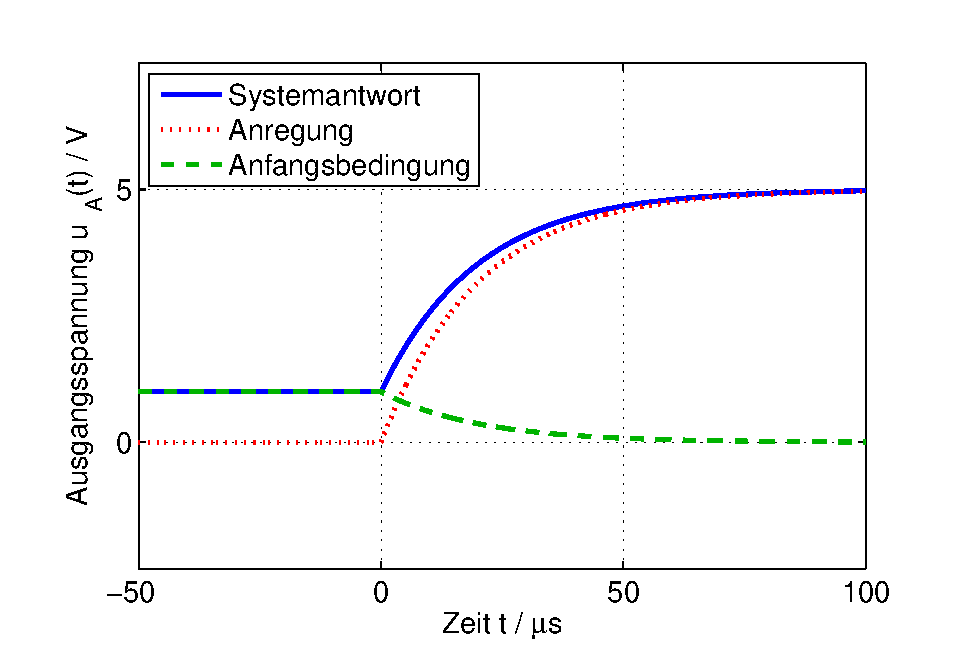
\includegraphics[width=0.5\textwidth]{Kapitel12/Bilder/image8}}
  \caption{Grafische Darstellung des Konvergenzintervalls f\"{u}r den Mittelwert f\"{u}r das Beispiel aus Tabelle \ref{tab:twelveone}}
  \label{fig:RegressionLinearOeltemperatur5}
\end{figure}

\subsubsection{Prognoseintervall f\"{u}r zuk\"{u}nftige Werte}

\noindent Um zuk\"{u}nftige Werte einer Stichprobe vorhersagen zu k\"{o}nnen, ist es erforderlich, das Prognoseintervall f\"{u}r die Reaktion $y_{N+1}$ an einer Stelle $x_{0}$ absch\"{a}tzen zu k\"{o}nnen. Die Lage eines zuk\"{u}nftigen Wertes ergibt sich aus dem Mittelwert und dem \"{u}berlagerten Messfehler. 

\begin{equation}\label{eq:twelveninetyfour}
y_{N+1} (x_{0})=b_{1} \cdot x_{0} +b_{0} +e=b_{1} \cdot (x_{0} -\bar{x})+\bar{y}+e
\end{equation}

\noindent Der Messfehler e ist mittelwertsfrei, sodass sich der Erwartungswert von 

\begin{equation}\label{eq:twelveninetyfive}
E\left(y_{N+1} (x_{0})\right)=E\left(b_{1} \cdot x_{0} +b_{0} +e\right)=E(b_{0})+E\left(b_{1} \cdot x_{0} \right)+E(e)=\beta _{0} +\beta _{1} \cdot x_{0}
\end{equation}

\noindent ergibt. Die Varianz der Gr\"{o}{\ss}e berechnet sich zu

\begin{equation}\label{eq:twelveninetysix}
\sigma _{y_{N+1}}^{2} =\sigma _{b_{1}}^{2} \cdot \left(x_{0} -\bar{x}\right)^{2} +\sigma _{\bar{y}}^{2} +\sigma ^{2} =\left(\dfrac{\left(x_{0} -\bar{x}\right)^{2} }{(N-1)\cdot s_{x}^{2}} +\dfrac{1}{N} +1\right)\cdot \sigma ^{2}
\end{equation}

\noindent Damit besitzt die Zufallsvariable 

\begin{equation}\label{eq:twelveninetyseven}
z=\dfrac{y_{N+1} (x_{0})-\left(b_{1} \cdot \left(x_{0} -\bar{x}\right)+\bar{y}\right)}{\sigma \cdot \sqrt{1+\dfrac{\left(x_{0} -\bar{x}\right)^{2}}{(N-1)\cdot s_{x}^{2}} +\dfrac{1}{N}}}
\end{equation}

\noindent eine Standardnormalverteilung. Die Varianz $\sigma^{2}$ wird mit Gleichung \eqref{eq:tenthirtyseven} gesch\"{a}tzt. Die Sch\"{a}tzung weist N - 2 Freiheitsgrade auf. Damit besitzt die Gr\"{o}{\ss}e 

\begin{equation}\label{eq:twelveninetyeight}
t=\dfrac{y_{N+1} (x_{0})-y_{0}}{\sqrt{\dfrac{\left(x_{0} -\bar{x}\right)^{2} }{(N-1)\cdot s_{x}^{2}} +\dfrac{N+1}{N}} \cdot \sqrt{\dfrac{a}{N-2}}}
\end{equation}

\noindent eine t-Verteilung mit N - 2 Freiheitsgraden auf, und die Standardabweichung $s_{yN+1}$ errechnet sich zu

\begin{equation}\label{eq:twelveninetynine}
s_{y_{N+1} } =\sqrt{\dfrac{\left(x_{0} -\bar{x}\right)^{2} }{(N-1)\cdot s_{x}^{2}} +\dfrac{N+1}{N}} \cdot \sqrt{\dfrac{a}{N-2}}
\end{equation}

\noindent Der Z\"{a}hler der Variable stellt den Abstand des Sch\"{a}tzwertes $y_{N+1}(x_{0})$ an der Stelle $x_{0}$ zu der Regressionsgeraden dar, sodass diese Zufallsvariable zur Bestimmung des Prognoseintervalls verwendet werden kann. 

\begin{equation}\label{eq:twelveonehundred}
P(c_{1} <t\le c_{2})=F(c_{2})-F(c_{1})=\gamma
\end{equation}

\noindent Durch die Symmetrie des Prognosebereichs ergeben sich die Konstanten $c_{1}$ und $c_{2}$ zu

\begin{equation}\label{eq:twelveonehundredone}
c_{1} =F^{-1} \left(\dfrac{1-\gamma }{2} \right)
\end{equation}

\noindent und

\begin{equation}\label{eq:twelveonehundredtwo}
c_{2} =F^{-1} \left(\dfrac{1-\gamma }{2} \right)
\end{equation}

\noindent Durch Umformungen ergibt sich ein Ausdruck f\"{u}r den Prognosebereich zuk\"{u}nftiger Stichprobenwerte

\begin{equation}\label{eq:twelveonehundredthree}
\gamma =P(c_{1} <t\le c_{2})=P\left(y(x_{0})+c_{1} \cdot s_{y_{N+1} } <y_{N+1} (x_{0})\le y(x_{0})+c_{2} \cdot s_{y_{N+1} } \right)
\end{equation}

\noindent mit

\begin{equation}\label{eq:twelveonehundredfour}
y(x_{0})=\left(b_{1} \cdot (x_{0} -\bar{x})+\bar{y}\right)
\end{equation}

\noindent Der Prognosebereich ist von der Zufallsvariablen x abh\"{a}ngig und erreicht seine minimale L\"{a}nge an der Stelle $x = \bar{x}$. Mit steigendem Abstand x von dem Mittelwert steigt die L\"{a}nge des Prognoseintervalls an.\newline

\noindent Ein Vergleich von Konfidenz- und Prognoseintervall zeigt, dass sie sich formell nur leicht unterscheiden. F\"{u}r den Konfidenzbereich des Mittelwertes existiert ein Summand 1 / N und bei der Berechnung des Prognoseintervalls f\"{u}r zuk\"{u}nftige Werte ein Summand (N + 1) / N. Da $N > 1$ ist, ist der Konfidenzbereich des Mittelwertes erwartungsgem\"{a}{\ss} kleiner als der Prognosebereich f\"{u}r zuk\"{u}nftige Werte. \newline

\noindent Das Verfahren ist in Tabelle \ref{tab:twelveeight} zusammengefasst.

\clearpage

\begin{table}[H]
\setlength{\arrayrulewidth}{.1em}
\caption{Vorgehen zur Bestimmung des Prognosebereiches f\"{u}r zuk\"{u}nftige Werte einer Regressionsgerade}
\setlength{\fboxsep}{0pt}%
\colorbox{lightgray}{%
\arrayrulecolor{white}%
\begin{tabular}{| wc{1cm} | wc{15.5cm} }
\xrowht{15pt}

\fontfamily{phv}\selectfont\textbf{Nr.} & 
\fontfamily{phv}\selectfont\textbf{Prozessschritt}\\ \hline \xrowht{20pt}

\fontfamily{phv}\selectfont{1} &
\fontfamily{phv}\selectfont{Wahl einer Konfidenzzahl $\gamma$} \\ \hline \xrowht{10pt}

\multirow{4}{*}{\fontfamily{phv}\selectfont{2}} &
\fontfamily{phv}\selectfont{Bestimmung der zugehörigen Parameter $c_{1}$ und $c_{2}$ aus der inversen t-Verteilung} \\ \xrowht{10pt}
&
\fontfamily{phv}\selectfont{mit N - 2 Freiheitsgraden} \\\xrowht{25pt}
& \fontfamily{phv}\selectfont{$c_{1} =F^{-1} \left(\dfrac{1-\gamma }{2} \right)  \qquad \qquad \qquad  $ und $\qquad \quad \qquad c_{2} =F^{-1} \left(\dfrac{1-\gamma }{2} \right)$}  \\ \hline \xrowht{20pt}

\multirow{4}{*}{\fontfamily{phv}\selectfont{3}} &
\fontfamily{phv}\selectfont{Berechnung der Mittelwerte der Stichprobe} \\\xrowht{35pt}
& \fontfamily{phv}\selectfont{$\bar{x}=\dfrac{1}{N} \cdot \sum _{n=1}^{N}x_{n} \qquad \qquad \qquad \qquad $ und $\qquad  \qquad  \qquad \qquad \bar{y}=\dfrac{1}{N} \cdot \sum _{n=1}^{N}y_{n}$}  \\ \hline \xrowht{20pt}

\multirow{4}{*}{\fontfamily{phv}\selectfont{4}} &
\fontfamily{phv}\selectfont{Bestimmung der Standardabweichung und der Kovarianz der Stichprobe} \\\xrowht{35pt}
& \fontfamily{phv}\selectfont{$s_{x} =\sqrt{\dfrac{1}{N-1} \cdot \sum _{n=1}^{N}\left(x_{n} -\bar{x}\right)^{2}}\qquad \qquad $ und $\qquad \qquad s_{xy} =\dfrac{1}{N-1} \cdot \left(\sum _{n=1}^{N}x_{n} \cdot y_{n} -N\cdot \bar{x}\cdot \bar{y}\right)$}  \\ \hline \xrowht{20pt}

\multirow{5}{*}{\fontfamily{phv}\selectfont{5}} &
\fontfamily{phv}\selectfont{Bestimmung der Parameter $b_{0}$ und $b_{1}$ der Regressionsgeraden} \\\xrowht{40pt}
& \fontfamily{phv}\selectfont{$b_{1} =\dfrac{\sum\limits _{n=1}^{N}x_{n} \cdot y_{n}  -N\cdot \bar{x}\cdot \bar{y}}{\sum\limits _{n=1}^{N}x_{n}^{2}  -N\cdot \bar{x}^{2} } =\dfrac{s_{xy} }{s_{x}^{2} }\qquad \qquad $ und $\qquad \qquad b_{0} =\bar{y}-b_{1} \cdot \bar{x}$}  \\ \hline \xrowht{20pt}

\multirow{4}{*}{\fontfamily{phv}\selectfont{6}} &
\fontfamily{phv}\selectfont{Berechnung der Fehlerquadratsumme} \\\xrowht{35pt}
& \fontfamily{phv}\selectfont{$a=\sum _{n=1}^{N}r_{n}^{2}  =\sum _{n=1}^{N}\left(y_{n} -b_{1} \cdot x_{n} -b_{0} \right)^{2}  $}  \\ \hline \xrowht{20pt}

\multirow{4}{*}{\fontfamily{phv}\selectfont{7}} &
\fontfamily{phv}\selectfont{Bestimmung der Standardabweichung} \\\xrowht{30pt}
& \fontfamily{phv}\selectfont{$s_{y_{N+1}} =\sqrt{\dfrac{(x_{0} -\bar{x})^{2}}{(N-1)\cdot s_{x}^{2}} +\dfrac{N+1}{N}} \cdot \sqrt{\dfrac{a}{N-2}}$}  \\ \hline \xrowht{20pt}

\multirow{4}{*}{\fontfamily{phv}\selectfont{8}} &
\fontfamily{phv}\selectfont{Bestimmung des  Prognoseintervalls} \\\xrowht{25pt}
& \fontfamily{phv}\selectfont{$y(x_{0})-c_{1} \cdot s_{y_{N+1}} \le \mu _{y_{N+1}} (x_{0})<y(x_{0})-c_{2} \cdot s_{y_{N+1}}$}  \\ \hline

\end{tabular}%
}\bigskip
\label{tab:twelveeight}
\end{table}

\clearpage

\noindent
\colorbox{lightgray}{%
\arrayrulecolor{white}%
\renewcommand\arraystretch{0.6}%
\begin{tabular}{ wl{16.5cm} }
{\fontfamily{phv}\selectfont
\noindent{Beispiel: Temperatursensor}}
\end{tabular}%
}\medskip 

\noindent Bild \ref{fig:RegressionLinearOeltemperatur6} zeigt die beiden Intervalle f\"{u}r das Beispiel des \"{O}ltemperatursensors aus Tabelle \ref{tab:twelveone}.

\noindent 
\begin{figure}[H]
  \centerline{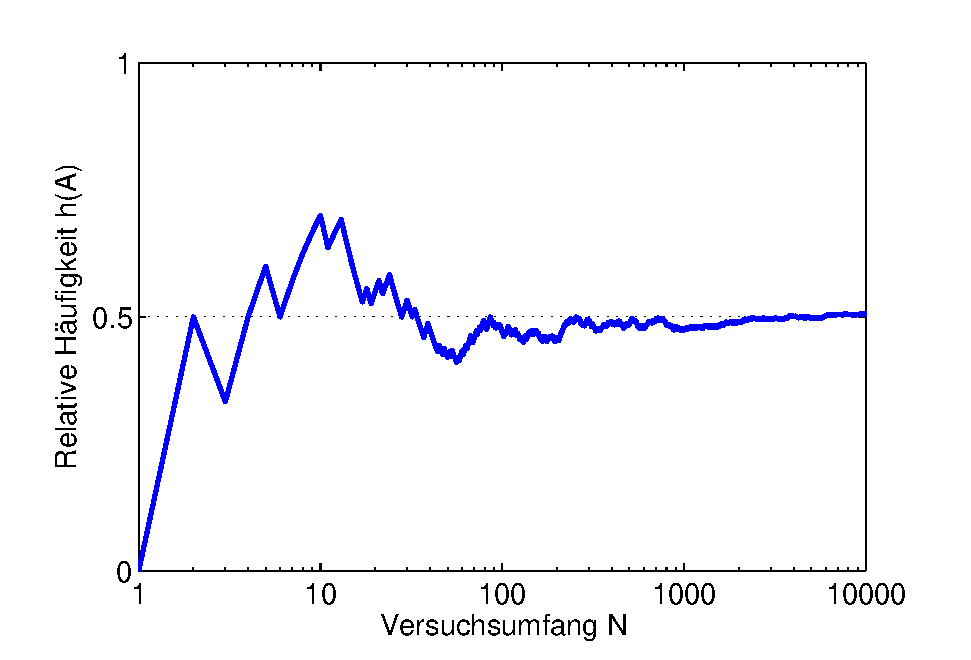
\includegraphics[width=0.5\textwidth]{Kapitel12/Bilder/image9}}
  \caption{Grafischer Vergleich des Konfidenzbereichs für den Mittelwert und des Prognosebereiches für zukünftige Werte bei einer Konfidenzzahl $\gamma = 0.95$}
  \label{fig:RegressionLinearOeltemperatur6}
\end{figure}

\subsubsection{Lineare Regression zweidimensionaler Datens\"{a}tze mit MATLAB}

\noindent MATLAB unterst\"{u}tzt die Regression zwei- und mehrdimensionaler Datens\"{a}tze mit einem umfangreichen Befehlssatz. Die wichtigsten Befehle sind in Tabelle \ref{tab:twelvenine} zusammengefasst.

\clearpage

\begin{table}[H]
\setlength{\arrayrulewidth}{.1em}
\caption{MATLAB-Befehle zur Berechnung und Bewertung von Regressionsfunktionen zweidimensionaler Datens\"{a}tze}
\setlength{\fboxsep}{0pt}%
\colorbox{lightgray}{%
\arrayrulecolor{white}%
\begin{tabular}{| c | c |}
\hline
\parbox[c][0.28in][c]{1.8in}{\smallskip\centering\textbf{\fontfamily{phv}\selectfont{Befehl}}} & 
\parbox[c][0.28in][c]{4.7in}{\smallskip\centering\textbf{\fontfamily{phv}\selectfont{Beschreibung}}}\\ \hline

\parbox[c][1.2in][c]{1.8in}{\centering{\fontfamily{phv}\selectfont{$[B,s] = polyfit(X,Y,M)$}}} &
\parbox[c][1.2in][c]{4.7in}{\fontfamily{phv}\selectfont{Polyfit berechnet zu einem Eingangsvektor X und einem Ausgangsvektor Y ein Regressionspolynom M-ter Ordnung, die Koeffizienten werden in dem Vektor B dargestellt. Au{\ss}erdem wird eine Struktur s erzeugt, die zur Berechnung von Konfidenzbereich des Mittelwertes und des Prognosebereiches zuk\"{u}nftiger Stichprobenwerte erforderlich ist}}\\ \hline

\parbox[c][0.8in][c]{1.8in}{\centering{\fontfamily{phv}\selectfont{$[Y,DEL] = polyval(B,X,s)$}}} &
\parbox[c][0.8in][c]{4.7in}{\fontfamily{phv}\selectfont{Polyval berechnet die Regressionswerte des Polynoms mit den Koeffizienten P an den Stelle X, au{\ss}erdem die Standardabweichung des Konfidenzintervalls des Mittelwertes, Basis sind die \"{u}ber polyfit berechneten Werte B und s}}\\ \hline

\parbox[c][1.2in][c]{1.8in}{\centering{\fontfamily{phv}\selectfont{$[Y,DEL] = polyconf(B,X,s)$}}} &
\parbox[c][1.2in][c]{4.7in}{\fontfamily{phv}\selectfont{Polyconf hat eine \"{a}hnliche Funktion wie polyval, erlaubt aber durch die Angabe der Schl\"{u}sselw\"{o}rter observation und curve auch die Berechnung zuk\"{u}nftiger Prognosewerte. Mit dem Schl\"{u}sselwort observation lassen sich die Prognoseintervalle und mit dem Schl\"{u}sselwort curve die Konfidenzintervalle berechnen. Als default Einstellung in MATLAB ist observation mit $\alpha = 5 \%$ definiert.}}\\ \hline

\parbox[c][1in][c]{1.8in}{\centering{\fontfamily{phv}\selectfont{$stats = regstats(Y,X,model)$}}} &
\parbox[c][1in][c]{4.7in}{\fontfamily{phv}\selectfont{Regstats liefert eine Datenstruktur zur Bewertung der Regression. Mit den Werten kann eine Signifikanzbewertung der Terme durchgef\"{u}hrt werden, und es k\"{o}nnen Konfidenzbereiche der Residuen angegeben werden. Au{\ss}erdem bietet sich die M\"{o}glichkeit der Bewertung \"{u}ber Bestimmtheitsma{\ss}e}}\\ \hline

\parbox[c][0.5in][c]{1.8in}{\centering{\fontfamily{phv}\selectfont{$[B,Bint] = regress(Y,X)$}}} &
\parbox[c][0.5in][c]{4.7in}{\fontfamily{phv}\selectfont{Regress berechnet die Regressionskoeffizienten und deren Konfidenzintervalle}}\\ \hline

\end{tabular}%
}
\label{tab:twelvenine}
\end{table}

\clearpage

\noindent F\"{u}r das Beispiel des Temperatursensors ergibt sich die folgende Befehlssequenz:

\lstinputlisting[caption = {}]{Kapitel12/mat1.m}

\noindent Zu beachten sind die unterschiedlichen Zusammensetzungen der Matrix von Eingangsgr\"{o}{\ss}en bei den Befehlen regstats und regress, dazu sind in der MATLAB-Hilfe detailliertere Information zu finden.\newline

\noindent Die Ergebnisse f\"{u}r die Regression entsprechen den analytisch berechneten Werten. Einige statistische Informationen des regstats-Befehls werden in den folgenden Abschnitten noch aufgegriffen.

\clearpage

\subsection{Regression mit Polynomen}

\noindent In Abschnitt 11.1 wird eine zweidimensionale Stichprobe \"{u}ber eine Gerade approximiert. Mithilfe statistischer Verfahren werden f\"{u}r die Regressionsparameter und den funktionalen Zusammenhang selbst Konfidenzbereiche bestimmt. 

\noindent Bei technischen Aufgabenstellungen ist es insbesondere bei Fehlerabsch\"{a}tzungen erforderlich, funktionale Zusammenh\"{a}nge h\"{o}herer Ordnung \"{u}ber Polynome beschreiben zu k\"{o}nnen. Dieser Ansatz f\"{u}hrt zur Regression mit Polynomen. 

\noindent Aus Gr\"{u}nden der \"{U}bersichtlichkeit werden f\"{u}r die Regression mit Polynomen in diesem Abschnitt keine statistischen Bewertungen hergeleitet. Zur Bewertung werden verf\"{u}gbare Verfahren aus Software-Paketen verwendet. Eine ausf\"{u}hrliche Herleitung ist in Kapitel \ref{twelve} zu finden.

\subsection{Berechnung und Bewertung der Regressionskoeffizienten}

\noindent Analog zum Vergehen zur Bestimmung einer Regressionsgeraden nach dem Prinzip des kleinsten Fehlerquadrates kann auch ein Polynom h\"{o}herer Ordnung als Regressionsfunktion verwendet werden. Im allgemeinen Fall ergibt sich ein Polynom M-ter Ordnung der Form 

\begin{equation}\label{eq:twelveonehundredfive}
y(x_{0} )=b_{0} +b_{1} \cdot x+...+b_{M} \cdot x^{M}
\end{equation}

\noindent Zur Bestimmung der Koeffizienten $b_{m}$ wird wieder gefordert, dass die Summe der quadratischen Fehler a ein Minimum aufweist. Diese Forderung f\"{u}hrt zu den M + 1 Gleichungen

\begin{equation}\label{eq:twelveonehundredsix}
\dfrac{\partial a}{\partial b_{0}} =0, \dfrac{\partial a}{\partial b_{1}} =0,\dots , \dfrac{\partial a}{\partial b_{M}} =0
\end{equation}

\noindent Zur Auswertung dieser Forderung stehen Software-Pakete zur Verf\"{u}gung, die neben der Bestimmung der Koeffizienten $b_{m}$ des Regressionspolynoms eine Berechnung des Konfidenzintervalls erlauben. Bild \ref{fig:RegressionLinearOeltemperatur7} zeigt die Regressionsfunktion f\"{u}r das Beispiel aus Tabelle \ref{tab:twelveone} mit der Ordnung M = 1, M = 2, M = 3, und M = 6.

\noindent 
\begin{figure}[H]
  \centerline{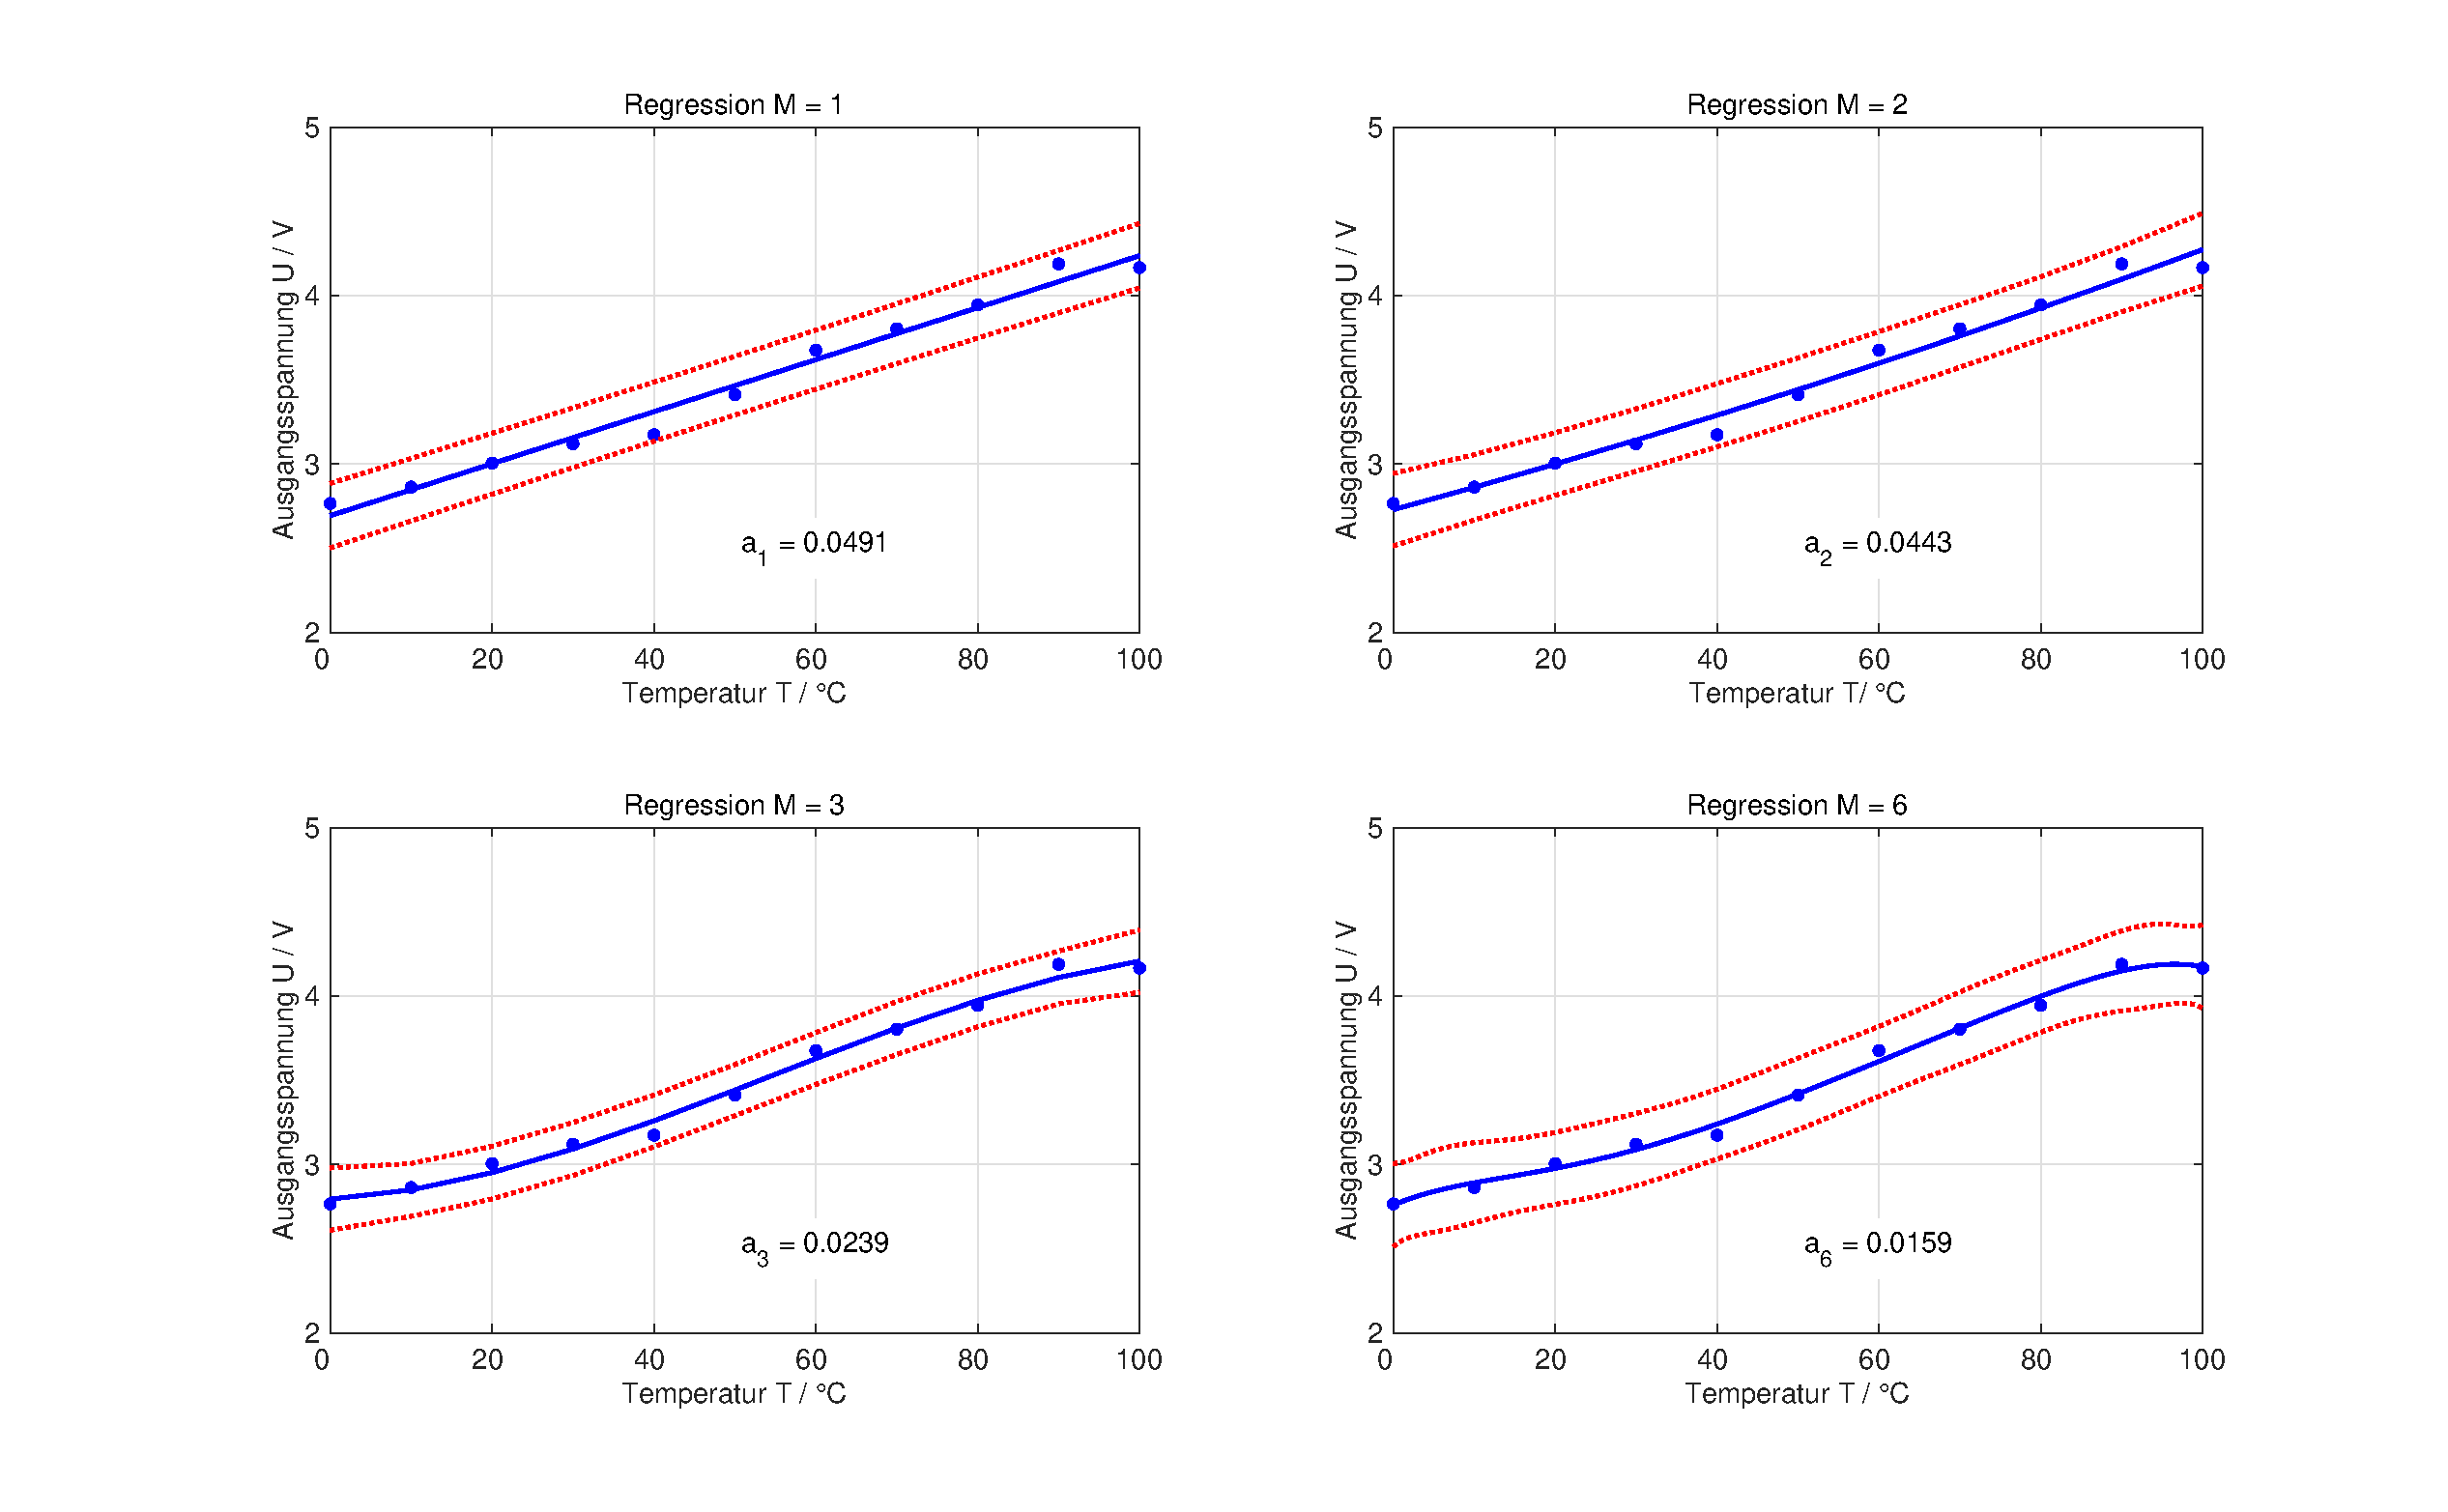
\includegraphics[width=1\textwidth]{Kapitel12/Bilder/image10}}
  \caption{Grafische Darstellung des Konvergenzintervalls f\"{u}r das Beispiel aus Tabelle 11.1 und Regressionspolynome der Ordnung M = 1, M = 2, M = 3 und M = 6, Vorhersagebereich mit $\gamma$ = 95 \%}
  \label{fig:RegressionLinearOeltemperatur7}
\end{figure}

\noindent In dem Beispiel sinkt die Summe der Fehlerquadrate mit steigender Ordnung M des Regressionspolynoms von $a_{1} = 0.0491$ auf $a_{6} = 0.0159$ ab. Generell wird die Summe der Fehlerquadrate mit steigender Ordnung des Polynoms immer sinken. Trotzdem muss der Ansatz eines Regressionspolynoms h\"{o}herer Ordnung nicht unbedingt zielf\"{u}hrend sein. Ergibt sich aus dem physikalischen Hintergrund ein linearer Zusammenhang, ist eine lineare Regressionsfunktion, die den physikalischen Zusammenhang beschreibt, sinnvoller als ein Regressionspolynom h\"{o}herer Ordnung, das lediglich die Messfehler gut approximiert. \"{U}ber die G\"{u}te einer Regression entscheidet deshalb neben der Summe der Fehlerquadrate das Ziel, das mit der Regression verfolgt wird.\newline

\noindent Sollen die Daten \"{u}ber den bekannten Datenbereich extrapoliert werden, ergibt sich ein weiterer Grund f\"{u}r eine Regression mit einer geringen Ordnung. Dazu zeigt Bild \ref{tab:twelvetwelve} f\"{u}r Regressionsfunktionen der Ordnung M = 1 und M = 3 den Konfidenzbereich bei Extrapolation der Daten.

\noindent 
\begin{figure}[H]
  \centerline{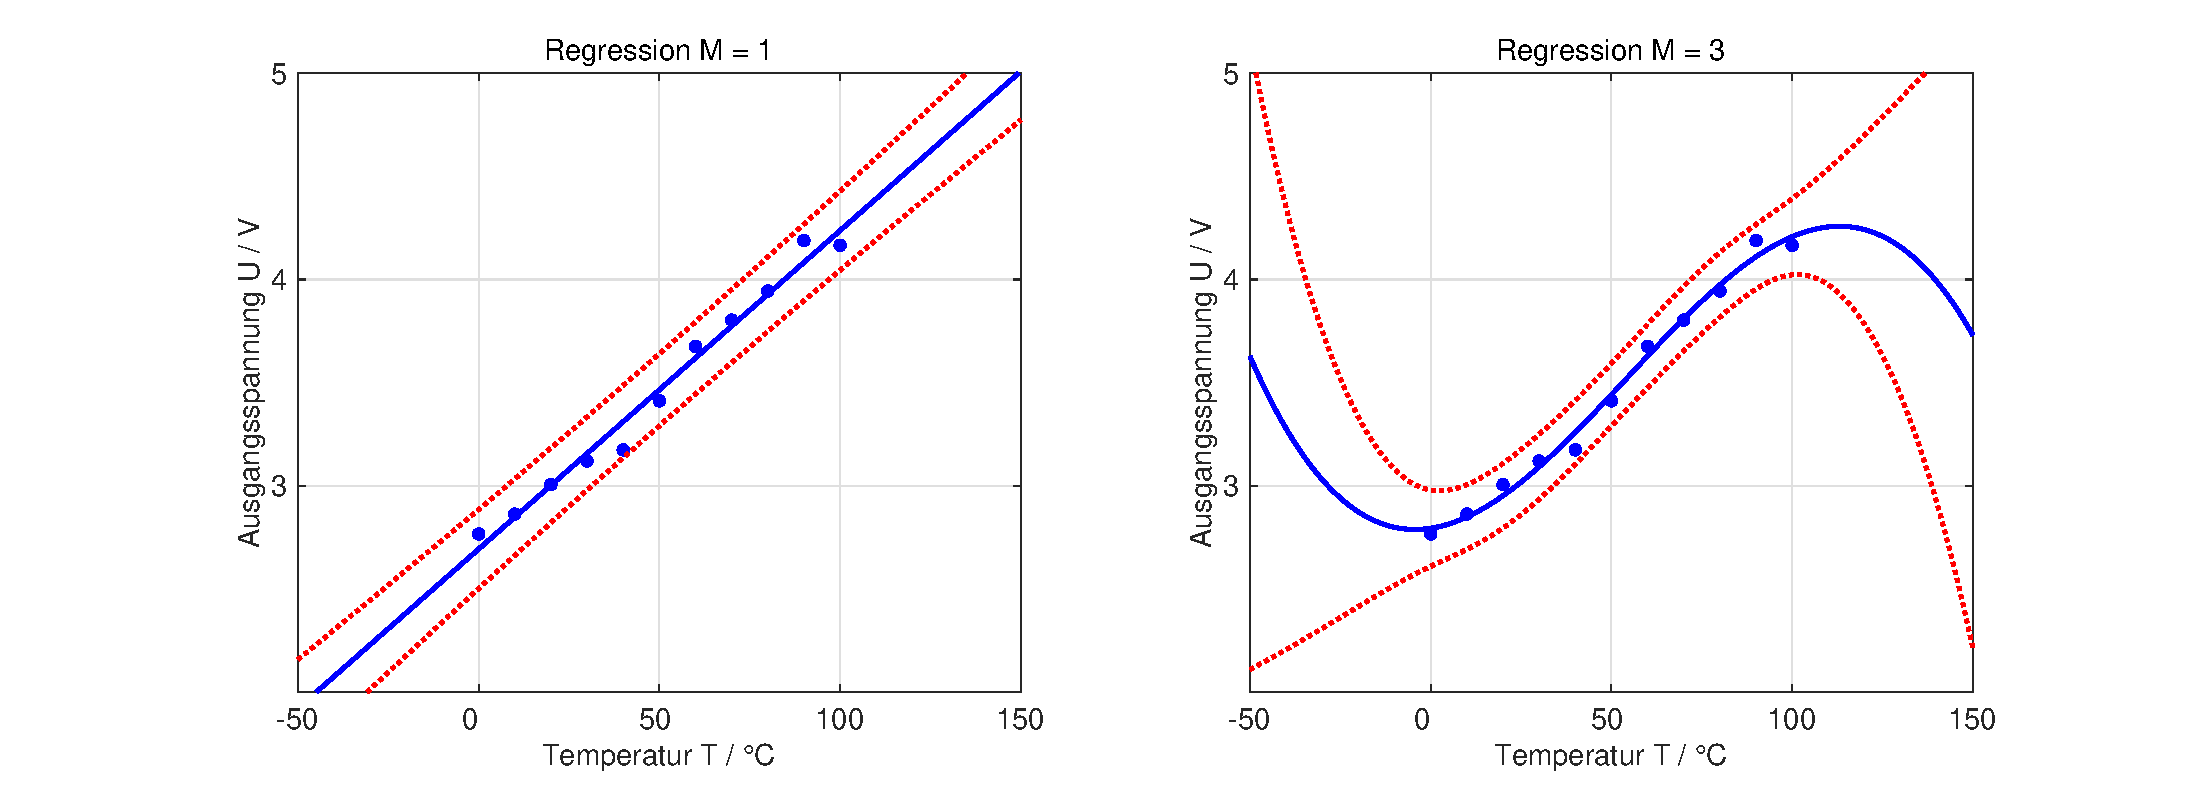
\includegraphics[width=1\textwidth]{Kapitel12/Bilder/image11}}
  \caption{Grafische Darstellung des Vorhersagebereichs mit $\gamma = 95 \%$ f\"{u}r das Beispiel aus Tabelle 11.1 und Regressionspolynome der Ordnung M = 1 und M = 3 bei Extrapolation}
  \label{fig:RegressionLinearOeltemperatur8}
\end{figure}

\noindent Es ist deutlich zu erkennen, dass das Konfidenzintervall bei Regressionsfunktionen h\"{o}herer Ordnung viel st\"{a}rker w\"{a}chst als bei Regressionen niedriger Ordnung. Daraus l\"{a}sst sich die Regel ableiten, die Regression mit einer m\"{o}glich geringen Ordnung zu realisieren und auf eine Extrapolation der Daten soweit wie m\"{o}glich zu vermeiden.\newline

\noindent Die Berechnung in MATLAB entspricht dem in Abschnitt 12.1.6 beschriebenen Vorgehen, es wird lediglich die Ordnung M des Polynoms ver\"{a}ndert.


\subsubsection{Signifikanz der einzelnen Regressionsterme bei Regressionsfunktionen h\"{o}herer Ordnung}

\noindent In dem Beispiel des Temperatursensors bleibt die Quadratsumme der Residuen bei einer Regression mit einem Polynom zweiter Ordnung $(a_{2} = 0.0443)$ fast genauso gro{\ss} wie bei einer Regression mit einer Geraden $(a_{1} = 0.0491)$. Wird als Regressionsfunktion ein Polynom dritter Ordnung verwendet, wird die Quadratsumme der Residuen $(a_{3} = 0.0239)$ praktisch halbiert. Offensichtlich scheint der quadratische Term weniger wichtig oder weniger signifikant zu sein als der kubische Term.\newline

\noindent Die Vermutung kann anhand der einzelnen Regressionskoeffizienten verifiziert werden. Die einzelnen Regressionskoeffizienten $b_{m}$ werden durch Minimierung des quadratischen Fehlers f\"{u}r die vorliegende Stichprobe gewonnen. Wegen des endlichen Stichprobenumfangs weisen die Regressionsparameter $b_{m}$ eine Unsicherheit auf, die durch die ihre Standardabweichung $s_{bm}$ ausgedr\"{u}ckt wird. Ist die Streuung $s_{bm}$ gegen\"{u}ber dem Regressionskoeffizienten $b_{m}$ klein, ist der Regressionskoeffizient $b_{m}$ mit hoher Wahrscheinlichkeit von null verschieden. \newline

\noindent Diese Entscheidung kann als Hypothesentest formuliert werden. Es wird die Nullhypothese getestet, dass der Regressionskoeffizient $b_{m}$den Wert null aufweist. In Tabelle \ref{tab:twelveten} wird dieser Test analog zu den Darstellungen in den Abschnitten 12.1.2 und 12.1.3 auf eine t-Verteilung mit N - 2 Freiheitsgraden und dem Signifikanzniveau $\alpha$ zur\"{u}ckgef\"{u}hrt. Ist die Wahrscheinlichkeit P kleiner als das Signifikanzniveau $\alpha$, wird davon ausgegangen, dass der Regressionskoeffizient signifikant ist. Andernfalls ist der Koeffizient f\"{u}r die Regression nicht von Bedeutung, er kann zu null gesetzt werden. Die Frage der Signifikanz eines Regressionsparameters wird bei vielen Software-Paketen als Koeffiziententabelle zusammengefasst. Tabelle \ref{tab:twelveten} stellt die Koeffiziententabelle f\"{u}r das Beispiel des \"{O}ltemperatursensors dar.

\clearpage

\begin{table}[H]
\setlength{\arrayrulewidth}{.1em}
\caption{Bewertung der Signifikanz von Regressionskoeffizienten f\"{u}r das Beispiel aus Tabelle \ref{tab:twelveone} mit einem Stichprobenumfang von n = 11 \"{u}ber den t-Test}
\setlength{\fboxsep}{0pt}%
\colorbox{lightgray}{%
\arrayrulecolor{white}%
\begin{tabular}{| c | c | c | c | c | c |}
\hline
\parbox[c][0.65in][c]{0.95in}{\smallskip\centering\textbf{\fontfamily{phv}\selectfont{Name}}} & 
\parbox[c][0.65in][c]{0.95in}{\smallskip\centering\textbf{\fontfamily{phv}\selectfont{Regressions-koeffizient b$_{m}$}}} & 
\parbox[c][0.65in][c]{0.95in}{\smallskip\centering\textbf{\fontfamily{phv}\selectfont{Standard-abweichung s$_{bm}$}}} & 
\parbox[c][0.65in][c]{0.95in}{\smallskip\centering\textbf{\fontfamily{phv}\selectfont{t-Wert}}} & 
\parbox[c][0.65in][c]{0.95in}{\smallskip\centering\textbf{\fontfamily{phv}\selectfont{p-Wert}}} & 
\parbox[c][0.65in][c]{0.95in}{\smallskip\centering\textbf{\fontfamily{phv}\selectfont{Signifikanz}}}\\ \hline

\parbox[c][0.3in][c]{0.95in}{\centering{\fontfamily{phv}\selectfont{$b_{0}$}}} &
\parbox[c][0.3in][c]{0.95in}{\centering{\fontfamily{phv}\selectfont{$2.7940$}}} &
\parbox[c][0.3in][c]{0.95in}{\centering{\fontfamily{phv}\selectfont{$5.1\cdot 10^{-2}$}}} &
\parbox[c][0.3in][c]{0.95in}{\centering{\fontfamily{phv}\selectfont{$53.7917$}}} &
\parbox[c][0.3in][c]{0.95in}{\centering{\fontfamily{phv}\selectfont{$2.0\cdot 10^{-10}$}}} &
\parbox[c][0.3in][c]{0.95in}{\centering{\fontfamily{phv}\selectfont{ja}}}\\ \hline

\parbox[c][0.3in][c]{0.95in}{\centering{\fontfamily{phv}\selectfont{$b_{1}$}}} &
\parbox[c][0.3in][c]{0.95in}{\centering{\fontfamily{phv}\selectfont{$0.0027$}}} &
\parbox[c][0.3in][c]{0.95in}{\centering{\fontfamily{phv}\selectfont{$4.7\cdot 10^{-3}$}}} &
\parbox[c][0.3in][c]{0.95in}{\centering{\fontfamily{phv}\selectfont{$0.5673$}}} &
\parbox[c][0.3in][c]{0.95in}{\centering{\fontfamily{phv}\selectfont{$0.5882$}}} &
\parbox[c][0.3in][c]{0.95in}{\centering{\fontfamily{phv}\selectfont{nein}}}\\ \hline

\parbox[c][0.3in][c]{0.95in}{\centering{\fontfamily{phv}\selectfont{$b_{2}$}}} &
\parbox[c][0.3in][c]{0.95in}{\centering{\fontfamily{phv}\selectfont{$2.96\cdot 10^{-4}$}}} &
\parbox[c][0.3in][c]{0.95in}{\centering{\fontfamily{phv}\selectfont{$1.13\cdot 10^{-4}$}}} &
\parbox[c][0.3in][c]{0.95in}{\centering{\fontfamily{phv}\selectfont{$2.6147$}}} &
\parbox[c][0.3in][c]{0.95in}{\centering{\fontfamily{phv}\selectfont{$0.0347$}}} &
\parbox[c][0.3in][c]{0.95in}{\centering{\fontfamily{phv}\selectfont{ja}}}\\ \hline

\parbox[c][0.3in][c]{0.95in}{\centering{\fontfamily{phv}\selectfont{$b_{3}$}}} &
\parbox[c][0.3in][c]{0.95in}{\centering{\fontfamily{phv}\selectfont{$- 1.8\cdot 10^{-6}$}}} &
\parbox[c][0.3in][c]{0.95in}{\centering{\fontfamily{phv}\selectfont{$7.44\cdot 10^{-7}$}}} &
\parbox[c][0.3in][c]{0.95in}{\centering{\fontfamily{phv}\selectfont{$- 2.4437$}}} &
\parbox[c][0.3in][c]{0.95in}{\centering{\fontfamily{phv}\selectfont{$0.0445$}}} &
\parbox[c][0.3in][c]{0.95in}{\centering{\fontfamily{phv}\selectfont{ja}}}\\ \hline

\end{tabular}%
}
\label{tab:twelveten}
\end{table}

\noindent Die Analyse zeigt, dass alle Regressionskoeffizienten au{\ss}er dem Koeffizienten $b_{1}$ unterhalb der Grenze von 5 \% liegen und damit signifikant sind. Alternativ kann der Konfidenzbereich der Regressionskoeffizienten untersucht werden. Liegt die Zahl null innerhalb des Konfidenzintervalls, ist der betreffende Regressionskoeffizient f\"{u}r die zu untersuchende Aufgabenstellung nicht signifikant.\newline

\noindent Die f\"{u}r eine Bewertung der Signifikanz erforderlichen Daten ergeben sich aus den MATLAB-Befehlen regstats beziehungsweise regress. Die Befehle sind in Abschnitt 11.1.6 beschrieben. Zur Bewertung der Signifikanz wird die strukturierte Variable stats verwendet.

\lstinputlisting[caption = {}]{Kapitel12/mat2.m}

\begin{table}[H]
\setlength{\arrayrulewidth}{.1em}
\caption{Bewertung der Signifikanz von Regressionskoeffizienten f\"{u}r das Beispiel aus Tabelle 11.1 mit einem Stichprobenumfang von N = 11 \"{u}ber den Konfidenzbereich der Regressionskoeffizienten}
\setlength{\fboxsep}{0pt}%
\colorbox{lightgray}{%
\arrayrulecolor{white}%
\begin{tabular}{wc{3cm} | wc{3cm} | wc{3cm} | wc{3cm} | wc{3cm} }
\xrowht{10pt}

\multirow{2}{*}{\fontfamily{phv}\selectfont\textbf{Name}}
& \multicolumn{3}{c|}{\fontfamily{phv}\selectfont\textbf{Konfidenzintervall}} &
\multirow{2}{*}{\fontfamily{phv}\selectfont\textbf{Signifikanz}}\\ \cline{2-4} \xrowht{10pt}


& \fontfamily{phv}\selectfont\textbf{Minimum} &
\fontfamily{phv}\selectfont\textbf{Mitte} & \fontfamily{phv}\selectfont\textbf{Maximum} & \\ \hline \xrowht{10pt}

\fontfamily{phv}\selectfont{$b_{0}$} &
\fontfamily{phv}\selectfont{$2.6711$} &
\fontfamily{phv}\selectfont{$2.7940$} &
\fontfamily{phv}\selectfont{$2.9168$} &
\fontfamily{phv}\selectfont{ja}\\ \hline \xrowht{10pt}

\fontfamily{phv}\selectfont{$b_{1}$} &
\fontfamily{phv}\selectfont{$-0.0085$} &
\fontfamily{phv}\selectfont{$0.0027$} &
\fontfamily{phv}\selectfont{$0.0139$} &
\fontfamily{phv}\selectfont{nein}\\ \hline \xrowht{10pt}

\fontfamily{phv}\selectfont{$b_{2}$} &
\fontfamily{phv}\selectfont{$0.28\cdot 10^{-4}$} &
\fontfamily{phv}\selectfont{$2.96\cdot 10^{-4}$} &
\fontfamily{phv}\selectfont{$5.64\cdot 10^{-4}$} &
\fontfamily{phv}\selectfont{ja}\\ \hline \xrowht{10pt}

\fontfamily{phv}\selectfont{$b_{3}$} &
\fontfamily{phv}\selectfont{$- 3.6\cdot 10^{-6}$} &
\fontfamily{phv}\selectfont{$- 1.8\cdot 10^{-6}$} &
\fontfamily{phv}\selectfont{$- 0.1\cdot 10^{-6}$} &
\fontfamily{phv}\selectfont{ja}\\ \hline

\end{tabular}%
}\bigskip
\label{tab:twelveeleven}
\end{table}

\noindent Die Analyse der Konfidenzintervalle best\"{a}tigt den Hypothesentest. Zur Reduzierung der Komplexit\"{a}t kann das Regressionsmodell der Ausgangsspannung des \"{O}ltemperatursensors deshalb vereinfacht werden, indem die linearen Terme in T aus dem Modell eliminiert werden. Aus der urspr\"{u}nglichen Regressionsfunktion dritter Ordnung

\begin{equation}\label{eq:twelveonehundredseven}
U(T)=b_{0} +b_{1} \cdot T+b_{2} \cdot T^{2} +b_{3} \cdot T^{3}
\end{equation}

\noindent wird damit die reduzierte Regressionsfunktion mit 

\begin{equation}\label{eq:twelveonehundredeight}
U(T)=b_{0} +b_{2} \cdot T^{2} +b_{3} \cdot T^{3}
\end{equation}

\noindent Die neuen Regressionskoeffizienten und ihre Konfidenzintervalle sind in Tabelle \ref{tab:twelvetwelve} zusammengefasst.

\begin{table}[H]
\setlength{\arrayrulewidth}{.1em}
\caption{Bewertung der Signifikanz von Regressionskoeffizienten f\"{u}r das Beispiel aus Tabelle \ref{tab:twelveone} mit einem Stichprobenumfang von N = 11 \"{u}ber den Konfidenzbereich der Regressionskoeffizienten}
\setlength{\fboxsep}{0pt}%
\colorbox{lightgray}{%
\arrayrulecolor{white}%
\begin{tabular}{wc{3cm} | wc{3cm} | wc{3cm} | wc{3cm} | wc{3cm} }
\xrowht{10pt}

\multirow{2}{*}{\fontfamily{phv}\selectfont\textbf{Name}}
& \multicolumn{3}{c|}{\fontfamily{phv}\selectfont\textbf{Konfidenzintervall}} &
\multirow{2}{*}{\fontfamily{phv}\selectfont\textbf{Signifikanz}}\\ \cline{2-4} \xrowht{10pt}


& \fontfamily{phv}\selectfont\textbf{Minimum} &
\fontfamily{phv}\selectfont\textbf{Mitte} & \fontfamily{phv}\selectfont\textbf{Maximum} & \\ \hline \xrowht{10pt}

\fontfamily{phv}\selectfont{$b_{0}$} &
\fontfamily{phv}\selectfont{$2.74$} &
\fontfamily{phv}\selectfont{$2.81$} &
\fontfamily{phv}\selectfont{$2.88$} &
\fontfamily{phv}\selectfont{ja}\\ \hline \xrowht{10pt}

\fontfamily{phv}\selectfont{$b_{1}$} &
\fontfamily{phv}\selectfont{$2.87\cdot 10^{-4}$} &
\fontfamily{phv}\selectfont{$3.58\cdot 10^{-4}$} &
\fontfamily{phv}\selectfont{$4.28\cdot 10^{-4}$} &
\fontfamily{phv}\selectfont{ja}\\ \hline \xrowht{10pt}

\fontfamily{phv}\selectfont{$b_{2}$} &
\fontfamily{phv}\selectfont{$- 1.91\cdot 10^{-6}$} &
\fontfamily{phv}\selectfont{$- 2.19\cdot 10^{-6}$} &
\fontfamily{phv}\selectfont{$-1.48\cdot 10^{-6}$} &
\fontfamily{phv}\selectfont{ja}\\ \hline

\end{tabular}%
}\bigskip
\label{tab:twelvetwelve}
\end{table}

\noindent Die Koeffizienten \"{a}ndern sich bei Weglassen des linearen Regressionsterms. Die Analyse zeigt, dass nach dem Streichen des linearen Terms alle \"{u}brigen Regressionsterme signifikant sind, was durch einen Hypothesentest best\"{a}tigt werden k\"{o}nnte. Die Analysen f\"{u}r die Signifikanz von Regressionskoeffizienten werden wie auch die Bestimmung der Regressionskoeffizienten selbst mit entsprechenden Software-Paketen durchgef\"{u}hrt. Die Bewertung basiert auf dem in Abschnitt 11.1 dargestellten Verfahren. Das Verfahren zur Reduktion der Regressionsfunktion auf signifikante Terme ist in Bild \ref{fig:AblaufdiagrammReduktionRegressionsfunktion} dargestellt.

\noindent 
\begin{figure}[H]
  \centerline{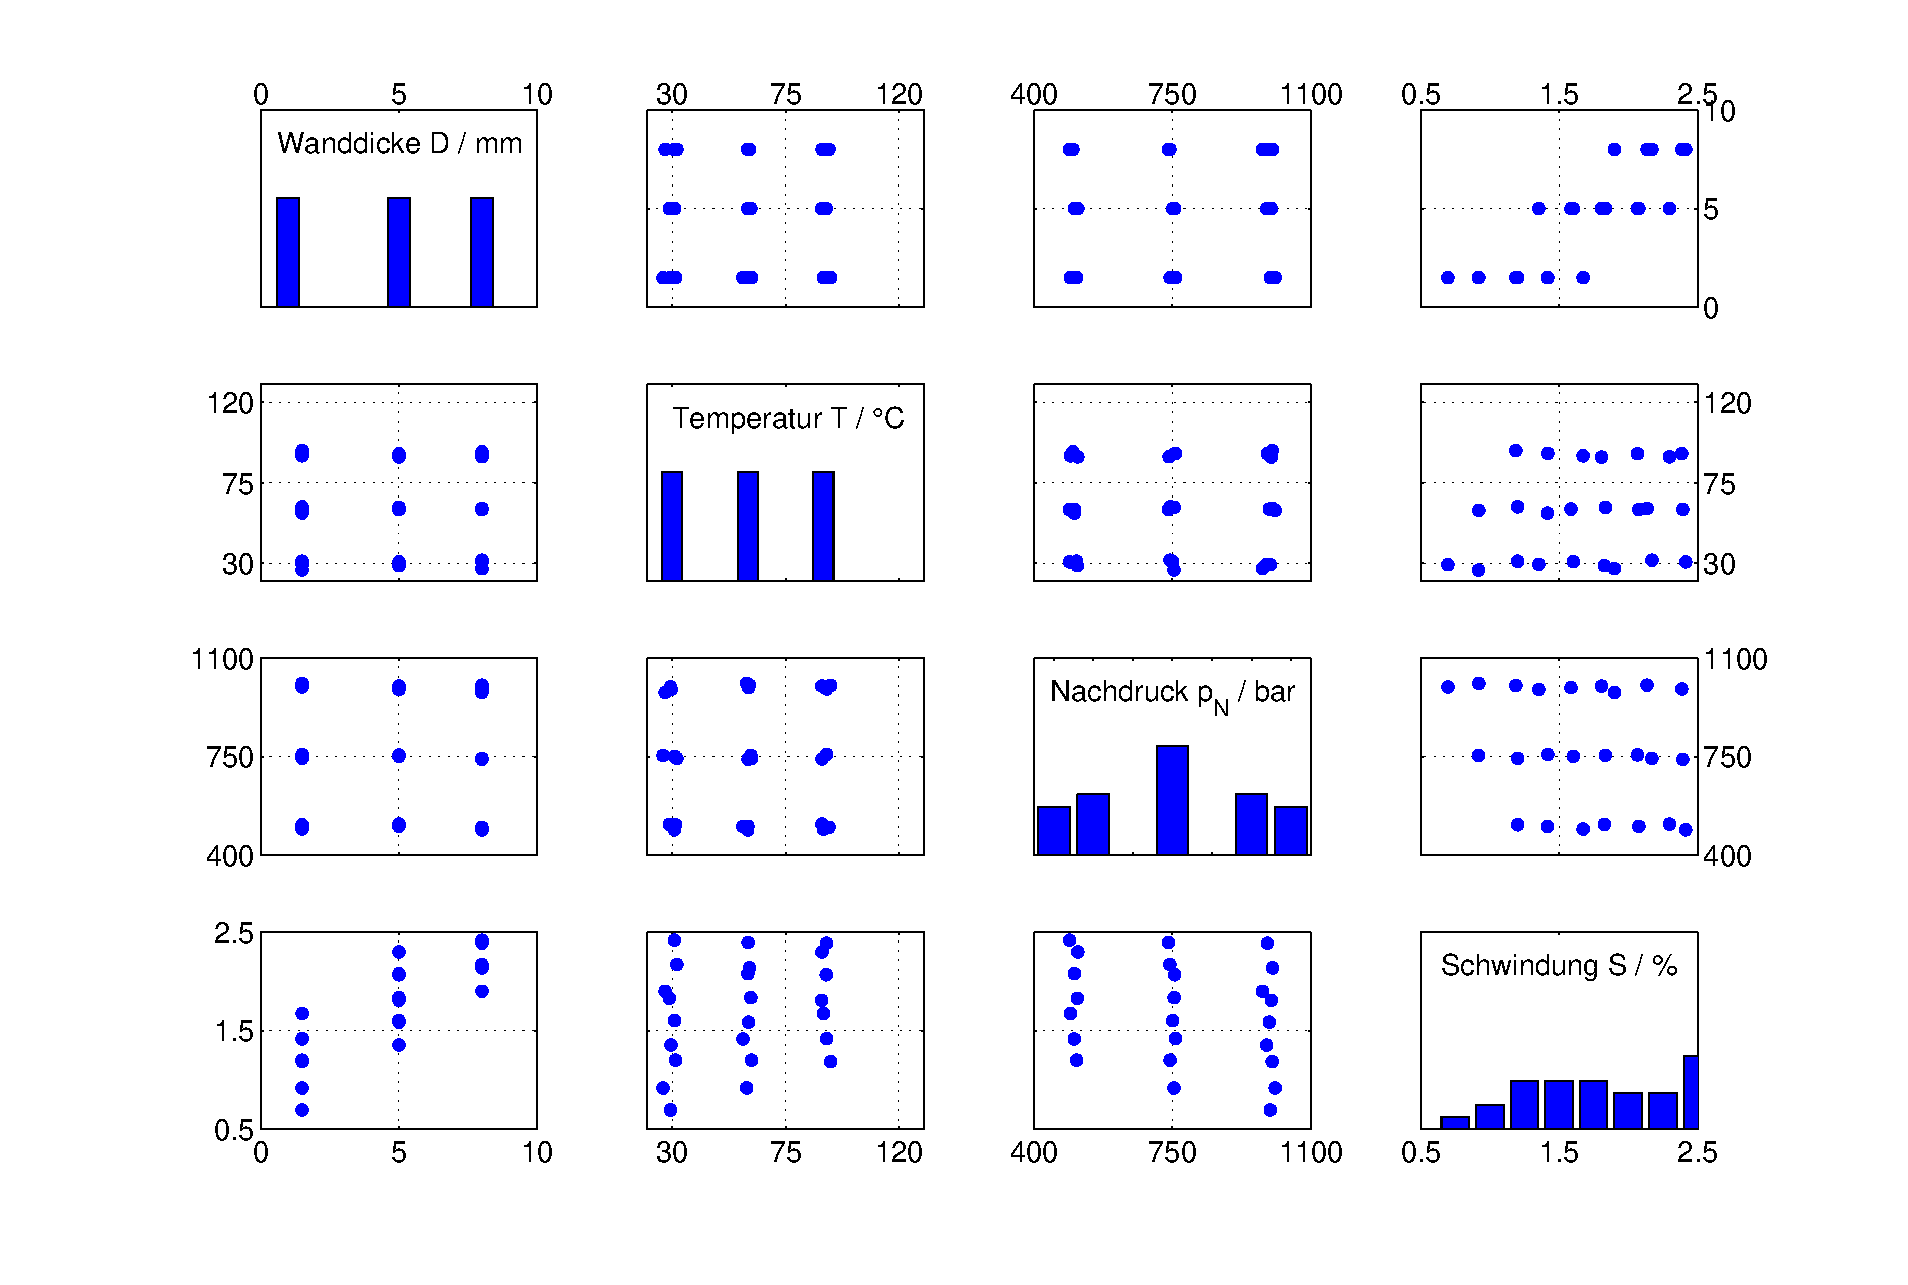
\includegraphics[width=0.6\textwidth]{Kapitel12/Bilder/image12}}
  \caption{Ablaufdiagramm zur Reduktion der Regressionsfunktion auf signifikante Terme}
  \label{fig:AblaufdiagrammReduktionRegressionsfunktion}
\end{figure}

\noindent Zun\"{a}chst wird eine Regressionsfunktion mit der gew\"{u}nschten Ordnung M erstellt. Mithilfe des beschriebenen t-Tests werden die einzelnen Terme hinsichtlich ihrer Signifikanz bewertet. Der Term mit dem h\"{o}chsten p-Wert ist am wenigsten signifikant, er wird eliminiert. Nach der Eliminierung dieses einzelnen Terms werden alle verbleibenden Terme erneut auf Signifikanz gepr\"{u}ft. Das Verfahren wird fortgesetzt, bis alle Terme signifikant sind, also einen p-Wert $< 5 \%$ aufweisen.

\clearpage

\subsection{Bewertung von Regressionen zweidimensionaler Datens\"{a}tze}

\noindent Nach Anpassung der Parameter muss das Ergebnis \"{u}berpr\"{u}ft und bewertet werden. Dazu werden verschiedene Fragestellungen betrachtet:

\begin{itemize}
    \item Wie gut ist die berechnete Regression?
    \item  Wie verh\"{a}lt sich die durch die Regression nicht erkl\"{a}rte Reststreuung? Welche Verteilung hat sie, existieren Ausrei{\ss}er? Welche Besonderheiten weist sie auf?
    \item  Entsprechen die Ergebnisse den physikalischen Vorstellungen, die \"{u}ber den Prozess bekannt sind?
\end{itemize}

\noindent Diese Fragestellungen werden in den folgenden Abschnitten diskutiert. Dabei wird zun\"{a}chst auf die Frage der Kenngr\"{o}{\ss}en f\"{u}r die G\"{u}te einer Regression eingegangen.

\subsubsection{Bewertung der Regressionsg\"{u}te \"{u}ber den Root-Mean-Square-Error}

\noindent Die Frage nach der G\"{u}te einer Regression kann \"{u}ber die Summe der quadratischen Fehler beantwortet werden. In dem Beispiel des \"{O}ltemperatursensors zeigt sich, dass mit zunehmender Ordnung M die Summe der quadratischen Fehler abnimmt. Die Summe der quadratischen Fehler ist demnach ein Ma{\ss} f\"{u}r die G\"{u}te der Regression. Um die Einheit der Zielgr\"{o}{\ss}e y zu erhalten, wird aus der Summe der quadratischen Fehler die Wurzel gezogen.\newline

\noindent Mit steigender Anzahl N von Messpunkten steigt die Summe der quadratischen Fehler stetig, obwohl die Regression aufgrund der gr\"{o}{\ss}eren Information immer besser wird. Um diesen Effekt zu kompensieren, muss die Wurzel der Summe von quadratischen Fehlern normiert werden. Durch diese Normierung ergibt sich ein Sch\"{a}tzwert f\"{u}r die Standardabweichung $s_{R}$ der Residuen.\newline

\noindent Liegt eine Regression der Ordnung M vor, m\"{u}ssen M + 1 Koeffizienten bestimmt werden. Weist die dazu vorhandene Stichprobe einen Umfang N auf, so muss zur eindeutigen Bestimmung der Koeffizienten die Bedingung

\begin{equation}\label{eq:twelveonehundrednine}
N\ge M+1
\end{equation}

\noindent erf\"{u}llt sein. Die Differenz 

\begin{equation}\label{eq:twelveonehundredten}
\nu =N-(M+1)=N-M-1
\end{equation}

\noindent beschreibt die Anzahl von Stichproben, die zur Absicherung des Regressionsergebnisses verwendet werden. F\"{u}r eine erwartungstreue Sch\"{a}tzung der Standardabweichung $s_{R}$ muss eine Normierung mit der Anzahl von Freiheitsgraden $\nu$ erfolgen. Damit ergibt sich die Standardabweichung der Residuen zu

\begin{equation}\label{eq:twelveonehundredeleven}
s_{R} =\sqrt{\dfrac{1}{N-M-1} \cdot \sum _{n=1}^{N}(y_{n} -y(x_{n}))^{2}}
\end{equation}

\noindent Sie wird auch als Root-Mean-Square-Error (RMS-Error) bezeichnet. Die Standardabweichung $s_{R}$ ist ein absolutes Ma{\ss} in den Einheiten der Zielgr\"{o}{\ss}e und damit ein absolutes Ma{\ss} f\"{u}r die Genauigkeit einer Regression. Um universelle G\"{u}tekriterien f\"{u}r Regressionen zu erhalten, die unabh\"{a}ngig von der zugrundeliegenden physikalischen Gr\"{o}{\ss}e sind, m\"{u}ssen deshalb weitere Kenngr\"{o}{\ss}en eingef\"{u}hrt werden.

\subsubsection{Bewertung der Regressionsg\"{u}te \"{u}ber das Bestimmtheitsma{\ss}}

\noindent Ein bew\"{a}hrtes Ma{\ss} der Statistik f\"{u}r die Bewertung von Streuungen ist die Varianz einer Zufallsvariable. Aus diesem Grund wird die Varianz der Stichprobenwerte $y_{n}$ analysiert.

\begin{equation}\label{eq:twelveonehundredtwelve}
s_{y}^{2} =\dfrac{1}{N-1} \cdot \sum _{n=1}^{N}(y_{n} -\bar{y})^{2}
\end{equation}

\noindent \"{A}hnlich wie bei der Varianzanalyse kann die Varianz der Stichprobenwerte in unterschiedliche Summanden zerlegt werden.

\begin{equation}\label{eq:twelveonehundredthirteen}
\begin{split}
(N-1)\cdot s_{y}^{2} & = \sum _{n=1}^{N}(y_{n} -\bar{y})^{2}  =\sum _{n=1}^{N}\left(y_{n} -y(x_{n} )+y(x_{n} )-\bar{y}\right)^{2}\\
& = \sum _{n=1}^{N}\left ((y_{n} -y(x_{n}))^{2} + 2\cdot (y_{n} -y(x_{n}))\cdot (y(x_{n})-\bar{y})+ (y(x_{n})-\bar{y})^{2} \right)\\
& = \sum _{n=1}^{N} (y_{n} -y(x_{n}))^{2}+2\cdot \sum _{n=1}^{N}\left ( (y_{n} -y(x_{n}))\cdot (y(x_{n})-\bar{y}) \right)+  \sum _{n=1}^{N} (y(x_{n})-\bar{y})^{2}
\end{split}
\end{equation}

\noindent Der mittlere Summand kann umgeformt werden zu

\begin{equation}\label{eq:twelveonehundredfourteen}
2\cdot \sum _{n=1}^{N}\left(\left(y_{n} -y(x_{n} )\right)\cdot \left(y(x_{n} )-\bar{y}\right)\right) =2\cdot \sum _{n=1}^{N}\left(r_{n} \cdot \left(y(x_{n} )-\bar{y}\right)\right) =2\cdot \sum _{n=1}^{N}\left(r_{n} \cdot y(x_{n})\right) -2\cdot \bar{y}\cdot \sum _{n=1}^{N}r_{n}
\end{equation}

\noindent Da die Summe der Residuen null ist, vereinfacht sich der Ausdruck zu

\begin{equation}\label{eq:twelveonehundredfifteen}
2\cdot \displaystyle\sum\limits _{n1}^{N}\left(\left(y_{n} -y(x_{n})\right)\cdot \left(y(x_{n})-\bar{y}\right)\right) =2\cdot \displaystyle\sum\limits _{n=1}^{N}\left(r_{n} \cdot y(x_{n})\right) -0
\end{equation}

\noindent Mit Gleichung \eqref{eq:twelvetwentyone} kann gezeigt werden, dass damit der gesamte Ausdruck zu null wird.

\begin{equation}\label{eq:twelveonehundredsixteen}
\begin{split}
2\cdot \displaystyle\sum\limits _{n=1}^{N}\left(r_{n} \cdot y(x_{n})\right) & = 2\cdot \displaystyle\sum\limits_{n=1}^{N}\left(r_{n} \cdot (b_{1} \cdot x_{n} +b_{0})\right) =2\cdot b_{1} \cdot \displaystyle\sum\limits _{n=1}^{N}(r_{n} \cdot x_{n}) +2\cdot b_{0} \cdot \displaystyle\sum\limits _{n=1}^{N}r_{n}\\
& = 2\cdot b_{1}\cdot \displaystyle\sum\limits_{n=1}^{N}(r_{n} \cdot x_{n}) + 0 = 2\cdot  b_{1}\cdot \displaystyle\sum\limits_{n=1}^{N} \left((y_{n}-y\left(x_{n})\right)\cdot x_{n}\right)\\
& = 2\cdot b_{1}\cdot \left((y_{n}-b_{1}\cdot x_{n} - b_{0})\cdot x_{n}\right)=0
\end{split}
\end{equation}

\noindent Die Varianz der Stichprobenwerte $y_{n}$ reduziert sich damit auf zwei Teilsummen

\begin{equation}\label{eq:twelveonehundredseventeen}
(N-1)\cdot s_{y}^{2} =\displaystyle\sum\limits _{n=1}^{N}\left(y_{n} -\bar{y}\right)^{2}  =\displaystyle\sum\limits _{n=1}^{N}\left(y_{n} -y(x_{n})\right)^{2}  +\displaystyle\sum\limits _{n=1}^{N}\left(y(x_{n})-\bar{y}\right)^{2}  =\displaystyle\sum\limits _{n=1}^{N}r_{n}^{2}  +\displaystyle\sum\limits _{n=1}^{N}\left(y(x_{n})-\bar{y}\right)^{2}
\end{equation}

\noindent Dabei ist der erste Summand die Quadratsumme der Residuen, der zweite Summand beschreibt die Quadratsumme der Sch\"{a}tzwerte. Division durch die linke Seite ergibt

\begin{equation}\label{eq:twelveonehundredeighteen}
1=\dfrac{\displaystyle\sum\limits _{n=1}^{N}r_{n}^{2}}{\displaystyle\sum\limits _{n=1}^{N}(y_{n} -\bar{y})^{2}} +\dfrac{\displaystyle\sum\limits_{n=1}^{N}\left(y(x_{n})-\bar{y}\right)^{2}}{\displaystyle\sum\limits _{n=1}^{N}(y_{n} -\bar{y})^{2}}
\end{equation}

\noindent Der erste Summand ist ein Ma{\ss} f\"{u}r die nicht erkl\"{a}rte Reststreuung. Der zweite Summand wird als Bestimmtheitsma{\ss} $R^{2}$ bezeichnet. 

\begin{equation}\label{eq:twelveonehundrednineteen}
R^{2} =\dfrac{N-1}{N-1} \cdot \dfrac{\displaystyle\sum\limits _{n=1}^{N}\left(y(x_{n})-\bar{y}\right)^{2}}{\displaystyle\sum\limits _{n=1}^{N}\left(y_{n} -\bar{y}\right)^{2}} =\dfrac{\dfrac{1}{N-1} \cdot \displaystyle\sum\limits _{n=1}^{N}\left(y(x_{n})-\bar{y}\right)^{2}  }{\dfrac{1}{N-1} \cdot \displaystyle\sum\limits_{n=1}^{N}\left(y_{n} -\bar{y}\right)^{2}} =\dfrac{\dfrac{1}{N-1} \cdot \displaystyle\sum\limits _{n=1}^{N}\left(y(x_{n})-\bar{y}\right)^{2}  }{\dfrac{1}{N-1} \cdot \displaystyle\sum\limits _{n=1}^{N}\left(y_{n} -\bar{y}\right)^{2}} =\dfrac{s_{y(x)}^{2}}{s_{y}^{2}}
\end{equation}

\noindent Es gibt an, welcher Anteil der Streuung mit der Regression beschrieben wird und liegt um Bereich $0 \le R^{2} \le 1$. Ein Bestimmtheitsma{\ss} $R^{2} = 1$ zeigt, dass die Prognosewerte mit den Stichprobenwerten perfekt \"{u}bereinstimmen. Bei einem Bestimmtheitsma{\ss} von $R^{2} = 0$ besteht kein Zusammenhang zwischen den \"{u}ber die Regressionsfunktion gesch\"{a}tzten Werten und den vorliegenden Stichprobenwerten.\newline

\noindent Das Bestimmtheitsma{\ss} w\"{a}chst mit steigender Anzahl von Regressionstermen stetig an. In Abschnitt 11.2.1 wird ausgef\"{u}hrt, dass eine Regression h\"{o}herer Ordnung nicht zwangsweise die bessere Regression ist. Deshalb wird das sogenannte adjungierte Bestimmtheitsma{\ss} eingef\"{u}hrt. 

\begin{equation}\label{eq:twelveonehundredtwenty}
R_{adj}^{2} =1-\dfrac{N-1}{N-M-1} \cdot (1-R^{2})
\end{equation}

\noindent F\"{u}r das Beispiel des \"{O}ltemperatursensors aus Tabelle \ref{tab:twelveone} ergeben sich folgende G\"{u}tekriterien f\"{u}r die unterschiedlichen Regressionen.

\begin{table}[H]
\setlength{\arrayrulewidth}{.1em}
\caption{G\"{u}tekriterien der unterschiedlichen Regressionen f\"{u}r das Beispiel des \"{O}ltemperatursensors mit einem Stichprobenumfang von N = 11}
\setlength{\fboxsep}{0pt}%
\colorbox{lightgray}{%
\arrayrulecolor{white}%
\begin{tabular}{| c | c | c | c | c | c |}
\hline
\parbox[c][0.65in][c]{0.95in}{\smallskip\centering\textbf{\fontfamily{phv}\selectfont{Ordnung \\
Regression}}} & 
\parbox[c][0.65in][c]{0.95in}{\smallskip\centering\textbf{\fontfamily{phv}\selectfont{FG}}} & 
\parbox[c][0.65in][c]{0.95in}{\smallskip\centering\textbf{\fontfamily{phv}\selectfont{a}}} & 
\parbox[c][0.65in][c]{0.95in}{\smallskip\centering\textbf{\fontfamily{phv}\selectfont{S$_{R}$}}} & 
\parbox[c][0.65in][c]{0.95in}{\smallskip\centering\textbf{\fontfamily{phv}\selectfont{R$^{2}$}}} & 
\parbox[c][0.65in][c]{0.95in}{\smallskip\centering\textbf{\fontfamily{phv}\selectfont{R$_{ADJ}^{2}$}}}\\ \hline

\parbox[c][0.3in][c]{0.95in}{\centering{\fontfamily{phv}\selectfont{$M = 1$}}} &
\parbox[c][0.3in][c]{0.95in}{\centering{\fontfamily{phv}\selectfont{$9$}}} &
\parbox[c][0.3in][c]{0.95in}{\centering{\fontfamily{phv}\selectfont{$0.0491$}}} &
\parbox[c][0.3in][c]{0.95in}{\centering{\fontfamily{phv}\selectfont{$0.0739$}}} &
\parbox[c][0.3in][c]{0.95in}{\centering{\fontfamily{phv}\selectfont{$0.9816$}}} &
\parbox[c][0.3in][c]{0.95in}{\centering{\fontfamily{phv}\selectfont{$0.9796$}}}\\ \hline

\parbox[c][0.3in][c]{0.95in}{\centering{\fontfamily{phv}\selectfont{$M = 2$}}} &
\parbox[c][0.3in][c]{0.95in}{\centering{\fontfamily{phv}\selectfont{$8$}}} &
\parbox[c][0.3in][c]{0.95in}{\centering{\fontfamily{phv}\selectfont{$0.0443$}}} &
\parbox[c][0.3in][c]{0.95in}{\centering{\fontfamily{phv}\selectfont{$0.0744$}}} &
\parbox[c][0.3in][c]{0.95in}{\centering{\fontfamily{phv}\selectfont{$0.9834$}}} &
\parbox[c][0.3in][c]{0.95in}{\centering{\fontfamily{phv}\selectfont{$0.99793$}}}\\ \hline

\parbox[c][0.3in][c]{0.95in}{\centering{\fontfamily{phv}\selectfont{$M = 3$}}} &
\parbox[c][0.3in][c]{0.95in}{\centering{\fontfamily{phv}\selectfont{$9$}}} &
\parbox[c][0.3in][c]{0.95in}{\centering{\fontfamily{phv}\selectfont{$0.0239$}}} &
\parbox[c][0.3in][c]{0.95in}{\centering{\fontfamily{phv}\selectfont{$0.0584$}}} &
\parbox[c][0.3in][c]{0.95in}{\centering{\fontfamily{phv}\selectfont{$0.9911$}}} &
\parbox[c][0.3in][c]{0.95in}{\centering{\fontfamily{phv}\selectfont{$0.9872$}}}\\ \hline

\end{tabular}%
}
\label{tab:twelvethirteen}
\end{table}

\noindent Das Bestimmtheitsma{\ss} und das adjungierte Bestimmtheitsma{\ss} zeigen, dass die Regression in allen F\"{a}llen einen sehr gro{\ss}en Anteil der Streuungen abgedeckt. An der Summe der quadratischen Fehler a wird aber auch deutlich, dass der \"{U}bergang von linearer Regression auf eine Regression der Ordnung M = 2 keinen wesentlichen Einfluss hat. 

\clearpage

\noindent MATLAB erlaubt die Berechnung des Bestimmtheitsma{\ss}es und des adjungierten Bestimmtheitsma{\ss}es mit dem Befehl regstats.

\lstinputlisting[caption = {}]{Kapitel12/mat3.m}

\subsection{Statistische Bewertung des Bestimmtheitsma{\ss}es}

\noindent F\"{u}r eine statistische Bewertung des Bestimmtheitsma{\ss}es wird ein Hypothesentest eingef\"{u}hrt. Er geht von der Nullhypothese H0 aus, dass die Regressionskoeffizienten $\beta_{m} = 0$ sind. Zur Bewertung wird wie bei der Varianzanalyse eine Zufallsvariable eingef\"{u}hrt, mit der das Verh\"{a}ltnis der erkl\"{a}rten Streuungen zu unerkl\"{a}rten Streuungen bewertet werden kann. Unter Ber\"{u}cksichtigung der Freiheitsgrade ergibt sich das Verh\"{a}ltnis der Varianzen zu

\begin{equation}\label{eq:twelveonehundredtwentyone}
v=\dfrac{\dfrac{1}{M} \cdot \displaystyle\sum\limits _{n=1}^{N}\left(y(x_{n})-\bar{y}\right)^{2}}{\dfrac{1}{N-M-1} \cdot \displaystyle\sum\limits _{n=1}^{N}\left(y_{n} -\hat{y}_{n} \right)^{2}} =\dfrac{\dfrac{1}{M} \cdot \displaystyle\sum\limits _{n=1}^{N}\left(y(x_{n})-\bar{y}\right)^{2}  }{\dfrac{1}{N-M-1} \cdot \displaystyle\sum\limits _{n=1}^{N}r_{n}^{2}} =\dfrac{\dfrac{1}{M} \cdot \displaystyle\sum\limits _{n=1}^{N}R^{2}  }{\dfrac{1}{N-M-1} \cdot \left(1-R^{2} \right)}
\end{equation}

\noindent Die Variable weist eine F-Verteilung mit (M, N - M - 1) Freiheitsgraden auf. Falls die Hypothese richtig ist, muss $R^{2}$ sehr klein sein. Zur Bewertung wird das Signifikanzniveau $\alpha$ herangezogen.

\begin{equation}\label{eq:twelveonehundredtwentytwo}
P(v<c)=F(c)=1-\alpha
\end{equation}

\noindent Die Grenze zur Annahme der Hypothese liegt mit der inversen F-Verteilung mit (M, N - M - 1) Freiheitsgraden damit bei

\begin{equation}\label{eq:twelveonehundredtwentythree}
c=F^{-1} (1-\alpha)
\end{equation}

\noindent Die Hypothese wird verworfen, wenn das vorliegende Bestimmtheitsma{\ss} zu einer Kenngr\"{o}{\ss}e

\begin{equation}\label{eq:twelveonehundredtwentyfour}
v_{0} =\dfrac{\dfrac{1}{M} \cdot \displaystyle\sum\limits _{n=1}^{N}R^{2}}{\dfrac{1}{N-M-1} \cdot \left(1-R^{2} \right)}
\end{equation}

\noindent f\"{u}hrt, die gr\"{o}{\ss}er als die Grenze c ist. Alternativ kann eine \"{U}berschreitungswahrscheinlichkeit p der Pr\"{u}fgr\"{o}{\ss}e $v_{0}$ bestimmt werden und mit dem Signifikanzniveau $\alpha$ verglichen werden. F\"{u}r einen signifikant von null verschiedenen Regressionskoeffizienten muss die Bedingungen

\begin{equation}\label{eq:twelveonehundredtwentyfive}
1-F(v_{0})<\alpha
\end{equation}

\noindent erf\"{u}llt werden. Damit l\"{a}sst sich der Test des Regressionskoeffizienten in folgenden Prozessschritten zusammenfassen.

\clearpage

\begin{table}[H]
\setlength{\arrayrulewidth}{.1em}
\caption{Test der Hypothese $R^{2} = 0$ gegen $R^{2} > 0$  f\"{u}r das Bestimmtheitsma{\ss} einer linearen Regression}
\setlength{\fboxsep}{0pt}%
\colorbox{lightgray}{%
\arrayrulecolor{white}%
\begin{tabular}{| wc{1cm} | wc{7.5cm} | wc{7.5cm}}
\xrowht{15pt}

\fontfamily{phv}\selectfont\textbf{Nr.} & 
\multicolumn{2}{c}{\fontfamily{phv}\selectfont\textbf{Prozessschritt}}\\ \hline \xrowht{20pt}

\fontfamily{phv}\selectfont{1} &
\multicolumn{2}{c}{\fontfamily{phv}\selectfont{Wahl eines Signifikanzniveaus $\alpha$}}\\ \hline \xrowht{10pt}

\multirow{4}{*}{\fontfamily{phv}\selectfont{2}} &
\multicolumn{2}{c}{\fontfamily{phv}\selectfont{Bestimmung des zugehörigen Parameters c aus der inversen F-Verteilung}} \\ \xrowht{10pt}
& \multicolumn{2}{c}{\fontfamily{phv}\selectfont{(M, N - M - 1) Freiheitsgraden}}  \\\xrowht{25pt}
& \multicolumn{2}{c}{\fontfamily{phv}\selectfont{$c=F^{-1} (1-\alpha)$}}  \\ \hline
\xrowht{20pt}

\multirow{4}{*}{\fontfamily{phv}\selectfont{3}} &
\multicolumn{2}{c}{\fontfamily{phv}\selectfont{Berechnung des Bestimmtheitsmaßes der Stichprobe}} \\ \xrowht{10pt}
& \multicolumn{2}{c}{\fontfamily{phv}\selectfont{$R^{2} =\dfrac{s_{\displaystyle y(x)}^{2}}{s_{\displaystyle y}^{2}}$}}  \\\hline\xrowht{20pt}

\multirow{5}{*}{\fontfamily{phv}\selectfont{4}} &
\multicolumn{2}{c}{\fontfamily{phv}\selectfont{Berechnung der Zufallsvariable für die Stichprobe}} \\ \xrowht{50pt}
& \multicolumn{2}{c}{\fontfamily{phv}\selectfont{$v_{0} =\dfrac{\dfrac{1}{M} \cdot \displaystyle\sum\limits _{n=1}^{N}R^{2}}{\dfrac{1}{N-M-1} \cdot (1-R^{2})}$}}  \\\hline\xrowht{10pt}

\multirow{6}{*}{\fontfamily{phv}\selectfont{5}}  &
\multirow{2}{*}{\fontfamily{phv}\selectfont{Bestimmung des Annahmebereichs}} & \fontfamily{phv}\selectfont{Berechnung des p-Values mit der} \\\xrowht{10pt}
& & \fontfamily{phv}\selectfont{F-Verteilung 
mit (M,N - M - 1) Freiheitsgraden} \\ \xrowht{40pt}
& \fontfamily{phv}\selectfont{$v_{0} \le c$ } & 
\fontfamily{phv}\selectfont{$p=F\left(v_{0} \right)$} \\ \hline\xrowht{15pt}

\multirow{4}{*}{\fontfamily{phv}\selectfont{6}}  &
\fontfamily{phv}\selectfont{F\"{u}r $v_{0} \leq c$ wird die Hypothese} & 
\fontfamily{phv}\selectfont{F\"{u}r $p \leq 1 - \alpha$ wird die Hypothese} \\ \xrowht{15pt}
& \fontfamily{phv}\selectfont{angenommen, f\"{u}r $v_{0} > c $ wird die} & \fontfamily{phv}\selectfont{angenommen, f\"{u}r $p > 1 -\alpha$ wird die } \\ \xrowht{15pt}
&  \fontfamily{phv}\selectfont{Hypothese verworfen} & \fontfamily{phv}\selectfont{Hypothese verworfen} \\ \hline

\end{tabular}%
}\bigskip
\label{tab:twelvefourteen}
\end{table}

\subsubsection{Bestimmtheitsma{\ss} und Korrelationskoeffizient}

\noindent In Kapitel \ref{nine} wird der Korrelationskoeffizient r als Ma{\ss} f\"{u}r die lineare Abh\"{a}ngigkeit zweier Gr\"{o}{\ss}en x und y eingef\"{u}hrt. 

\begin{equation}\label{eq:twelveonehundredtwentysix}
r=\dfrac{s_{xy}}{s_{x} \cdot s_{y}}
\end{equation}

\noindent Im Fall einer linearen Regression wird erwartet, dass die Stichprobenwerte $y_{n}$ und die Sch\"{a}tzwerte $y(x_{n})$ eine gro{\ss}e Korrelation aufweisen. Andererseits wird im vorangegangenen Abschnitt das Bestimmtheitsma{\ss} $R^{2}$ als Kenngr\"{o}{\ss}e f\"{u}r die G\"{u}te der Regression eingef\"{u}hrt.

\begin{equation}\label{eq:twelveonehundredtwentyseven}
R^{2} =\dfrac{\dfrac{1}{N-1} \cdot \sum _{n=1}^{N}\left(y(x_{n})-\bar{y}\right)^{2}  }{\dfrac{1}{N-1} \cdot \sum _{n=1}^{N}\left(y_{n} -\bar{y}\right)^{2}} =\dfrac{s_{y(x)}^{2}}{s_{y}^{2}}
\end{equation}

\noindent Bereits durch die Definitionen in Gleichung \eqref{eq:twelveonehundredtwentysix} und Gleichung \eqref{eq:twelveonehundredtwentyseven} kann ein Zusammenhang der beiden Kenngr\"{o}{\ss}en erahnt werden. Ausgehend von der empirischen Varianz der Sch\"{a}tzung

\begin{equation}\label{eq:twelveonehundredtwentyeight}
s_{y(x)}^{2} =\dfrac{1}{N-1} \cdot \sum _{n=1}^{N}\left(y(x_{n})-\bar{y}\right)^{2}
\end{equation}

\noindent kann durch Umformen der vereinfachte Ausdruck in Abh\"{a}ngigkeit der Stichprobenvarianz der Gr\"{o}{\ss}e x gefunden werden.

\begin{equation}\label{eq:twelveonehundredtwentynine}
\begin{split}
s_{y(x)}^{2} & =\dfrac{1}{N-1} \cdot \sum _{n=1}^{N}\left(y(x_{n})-\bar{y}\right)^{2}  =\dfrac{1}{N-1} \cdot \sum _{n=1}^{N}\left(b_{1} \cdot (x_{n} -\bar{x})+\bar{y}-\bar{y}\right)^{2}
\end{split}
\end{equation}

\noindent Mit der Definition des Regressionsparameters $b_{1}$ aus Gleichung \eqref{eq:twelveeighteen}

\begin{equation}\label{eq:twelveonehundredthirty}
b_{1} =\dfrac{s_{xy}}{s_{x}^{2}}
\end{equation}

\noindent folgt aus Gleichung \eqref{eq:twelveonehundredthirty} 

\begin{equation}\label{eq:twelveonehundredthirtyone}
s_{y(x)}^{2} =\dfrac{s_{xy}^{2}}{s_{x}^{4}} \cdot s_{x}^{2} =\dfrac{s_{xy}^{2}}{s_{x}^{2}}
\end{equation}

\noindent Mit der Definitionsgleichung des Bestimmtheitsma{\ss}es $R^{2}$ und Gleichung \eqref{eq:twelveonehundredthirtyone} ergibt sich bei linearer Regressionsfunktion der Zusammenhang zwischen dem Bestimmtheitsma{\ss} $R^{2}$ und dem Korrelationskoeffizienten r aus Kapitel \ref{nine}

\begin{equation}\label{eq:twelveonehundredthirtytwo}
R^{2} =\dfrac{s_{y(x)}^{2}}{s_{y}^{2}} =\dfrac{s_{xy}^{2}}{s_{x}^{2} \cdot s_{y}^{2}} =r^{2}
\end{equation}

\noindent Bei einer linearen Regression entspricht das Bestimmtheitsma{\ss} $R^{2}$ dem Quadrat des Korrelationskoeffizienten $r^{2}$.

\subsubsection{Reststreuungsanalyse}

\noindent Die Reststreuungsanalyse dient dazu, die durch das Modell nicht erkl\"{a}rte Streuung eingehender zu untersuchen. Sie basiert auf den Residuen $r_{n}$, also den Abweichungen zwischen den Stichprobenwerten und den entsprechenden Werten der Regressionsfunktion. 

\begin{equation}\label{eq:twelveonehundredthirtythree}
r_{n} =y_{n} -y(x_{n})
\end{equation}

\noindent Die Residuen spiegeln die in der Regression nicht abgebildeten Abweichungen wieder. Mit ihnen l\"{a}sst sich entscheiden, ob die Modellannahmen korrekt sind, und es lassen sich eventuelle Besonderheiten erkennen. Bild \ref{fig:RegressionLinearOeltemperatur9} stellt f\"{u}r das Beispiel des \"{O}ltemperatursensors die Residuen f\"{u}r eine lineare Regressionsfunktion dar.

\noindent 
\begin{figure}[H]
  \centerline{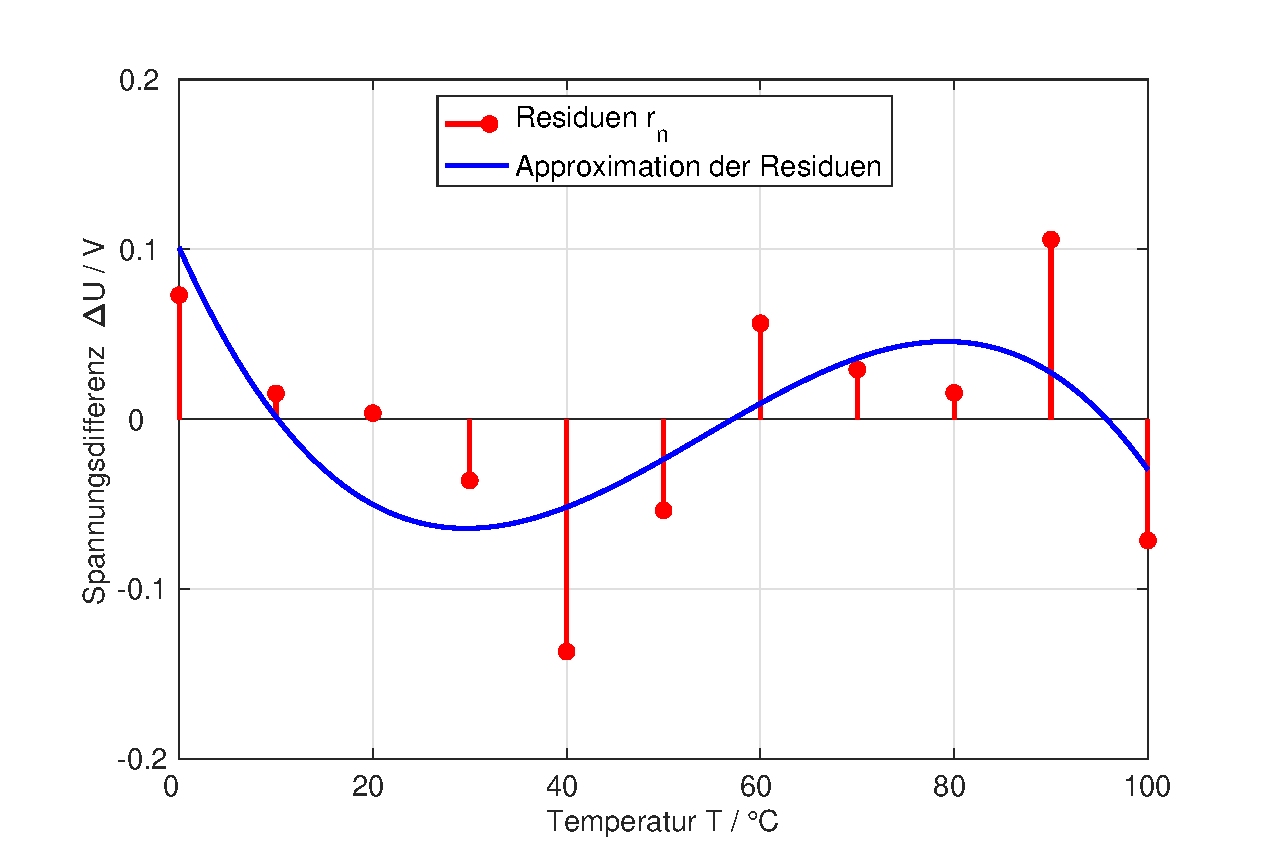
\includegraphics[width=0.5\textwidth]{Kapitel12/Bilder/image13}}
  \caption{Approximation der Residuen f\"{u}r das Beispiel des \"{O}ltemperatursensors durch ein Polynom h\"{o}herer Ordnung}
  \label{fig:RegressionLinearOeltemperatur9}
\end{figure}

\noindent Die Residuen zeigen einen Verlauf, der durch ein Polynom dritter Ordnung beschrieben werden kann. Die Reststreuungsanalyse zeigt damit, dass eine Regressionsfunktion h\"{o}herer Ordnung das Regressionsergebnis weiter verbessern w\"{u}rde. 

\noindent Bild \ref{fig:Residuenanalyse} stellt als weiteres Beispiel die lineare Regression von konstruierten Stichprobenwerten sowie die Residuen der Regression dar. Die Stichprobenwerte k\"{o}nnten zum Beispiel zwei Merkmale x und y eines Produktes als Funktion des Fertigungszeitpunktes beschreiben. Zwischen den Gr\"{o}{\ss}en x und y soll aus physikalischen Gr\"{u}nden n\"{a}herungsweise ein linearer Zusammenhang existieren. F\"{u}r die Stichprobenwerte wird eine lineare Regression durchgef\"{u}hrt und die Residuen werden bestimmt. Bild \ref{fig:Residuenanalyse} stellt das Ergebnis dar.

\noindent 
\begin{figure}[H]
  \centerline{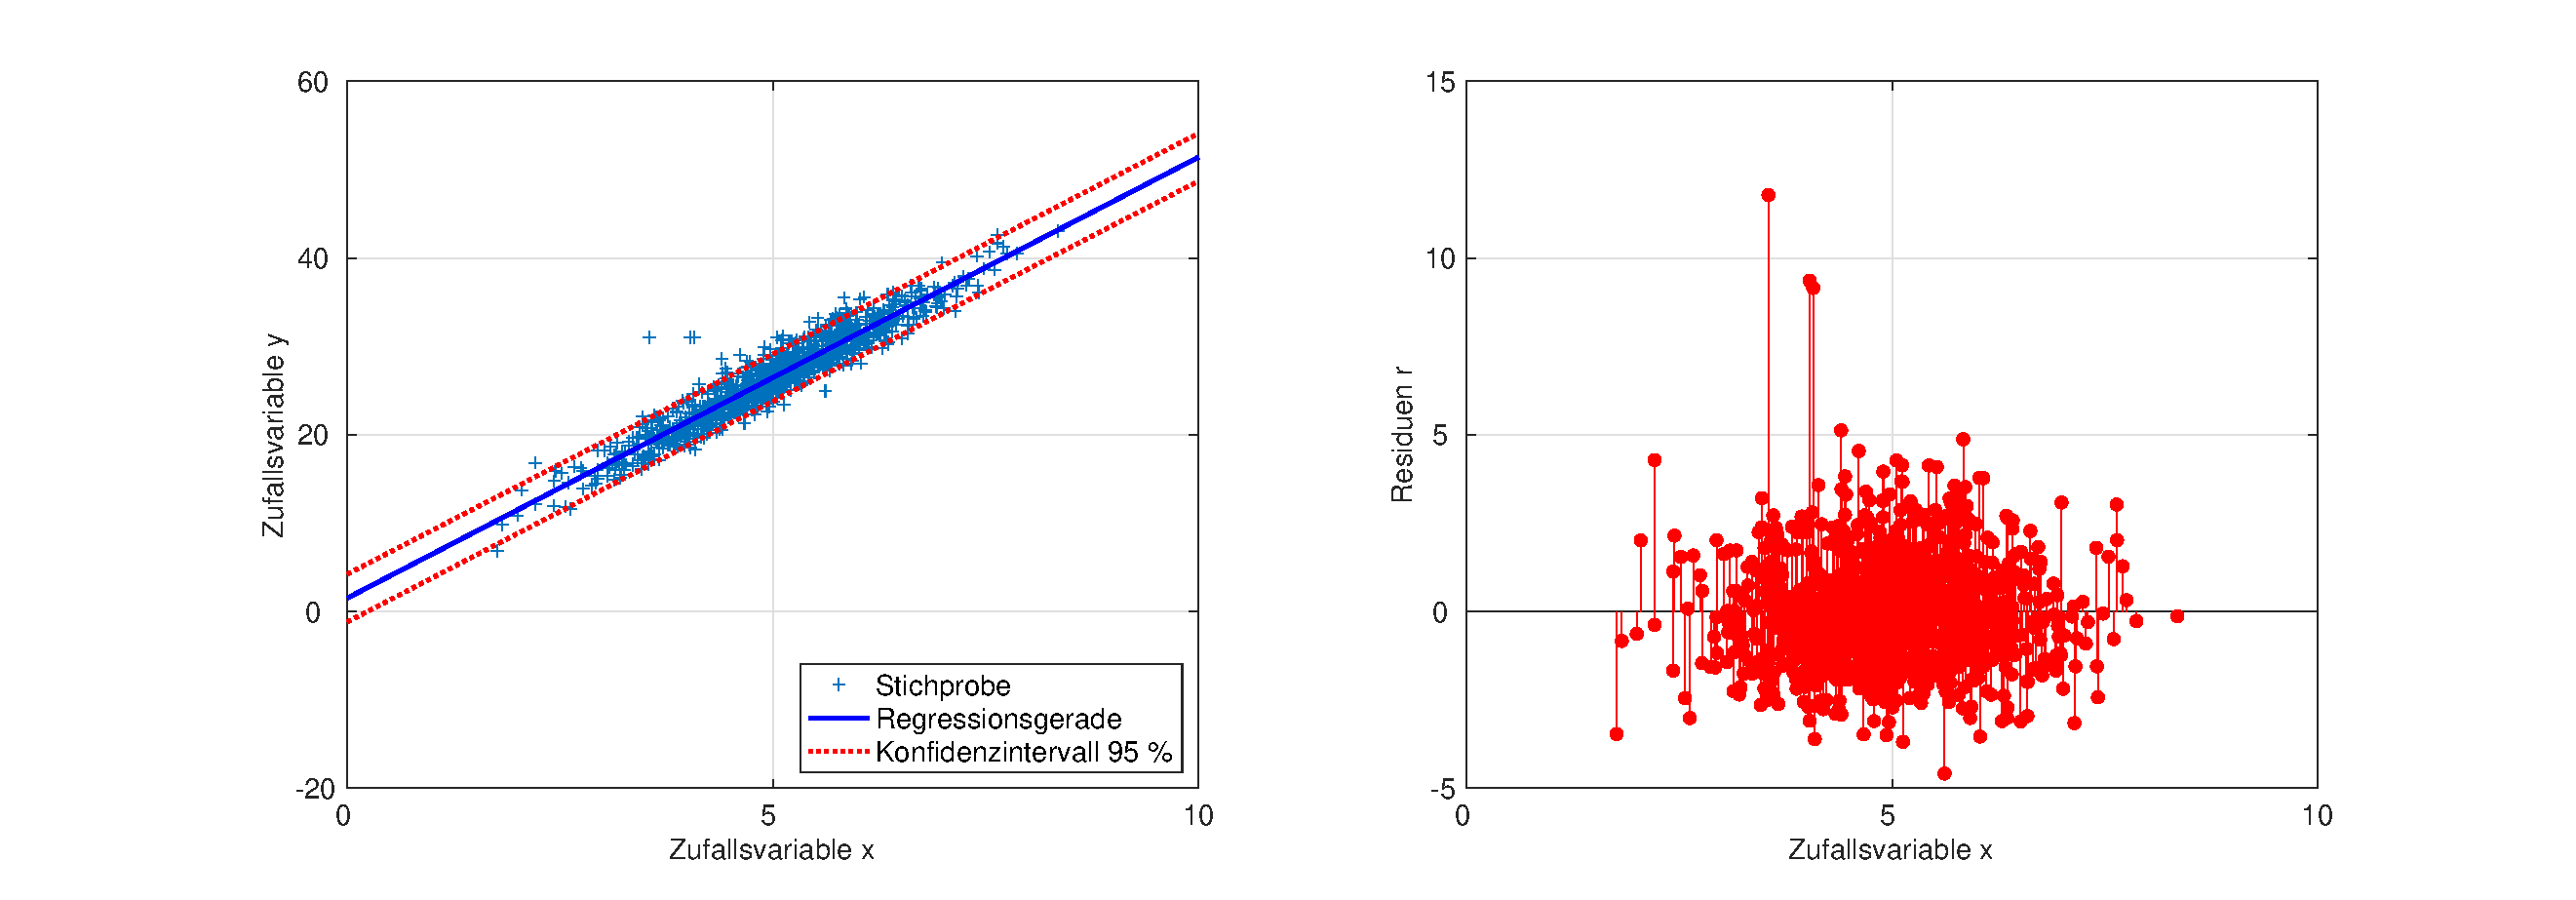
\includegraphics[width=1\textwidth]{Kapitel12/Bilder/image14}}
  \caption{Darstellung eines Testdatensatzes mit linearer Regression und den zugeh\"{o}rigen Residuen}
  \label{fig:Residuenanalyse}
\end{figure}

\noindent Die Residuen in Bild \ref{fig:Residuenanalyse} werden zun\"{a}chst plausibilisiert. Die Punkte liegen \"{u}ber den betrachteten Bereich auf ungef\"{a}hr konstantem Niveau. W\"{u}rden die Residuen wie bei dem Beispiel zum \"{O}ltemperatursensor einen bogenf\"{o}rmigen Verlauf aufweisen, w\"{a}re dies ein Hinweis darauf, dass die Ordnung der Regressionsfunktion nicht ausreichend ist. Die Ergebnisse hier zeigen, dass die Wahl der Regressionsfunktion sinnvoll ist. Deshalb wird vermutet, dass auch der physikalische Hintergrund auf einen linearen Zusammenhang zwischen den Zufallsvariablen x und y hinweist.\newline

\noindent Nach der ersten Plausibilisierung werden die Residuen auf Ausrei{\ss}er gepr\"{u}ft. Dazu werden die Residuen in Bild \ref{fig:Residuenanalyse2} als Box-Plot dargestellt.

\noindent 
\begin{figure}[H]
  \centerline{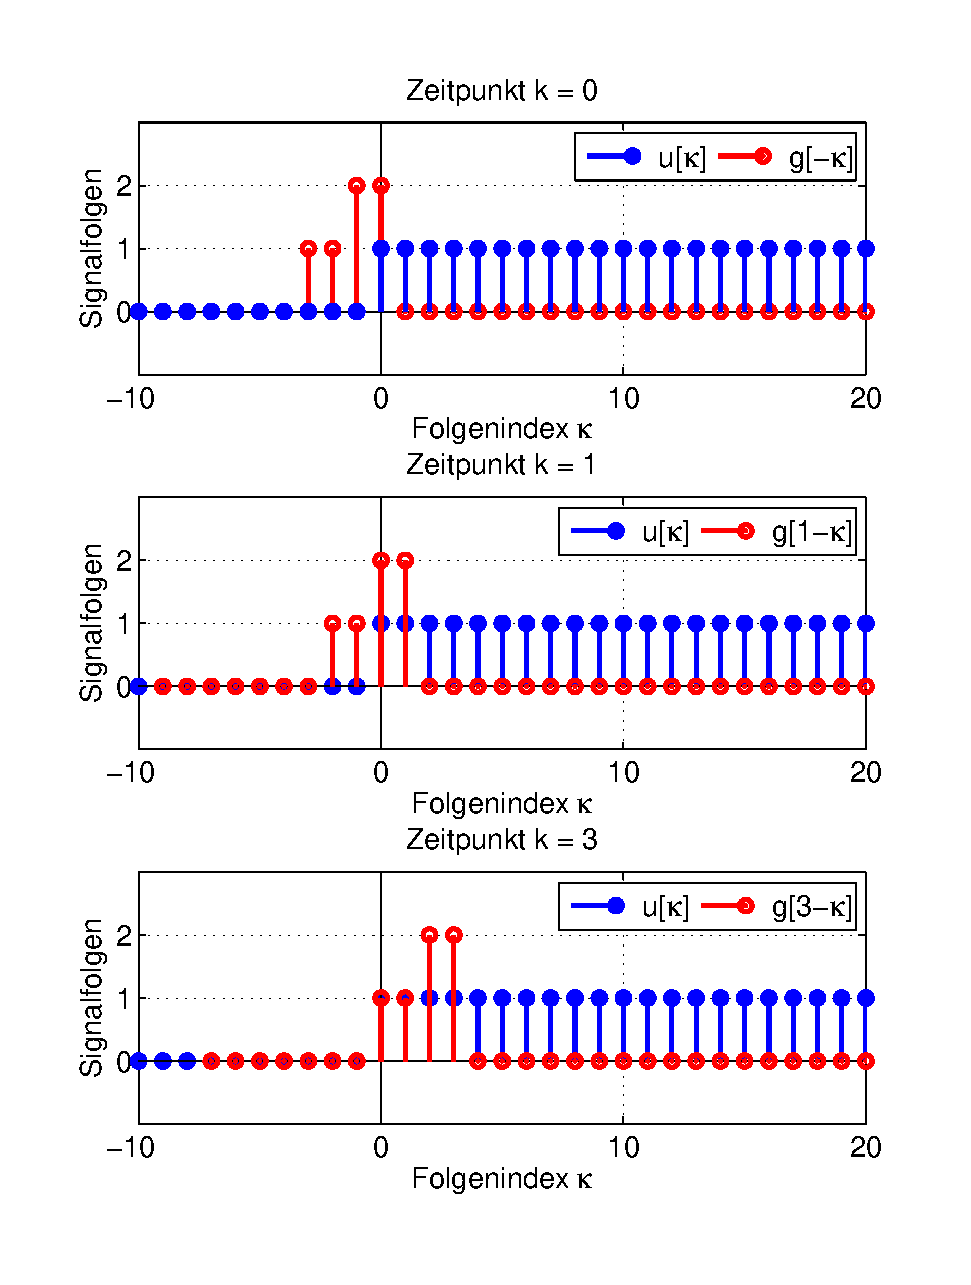
\includegraphics[width=0.5\textwidth]{Kapitel12/Bilder/image15}}
  \caption{Darstellung der Residuen einer Stichprobe als Box-Plot}
  \label{fig:Residuenanalyse2}
\end{figure}

\noindent Bei dem Box-Plot werden einzelne Stichprobenwerte als Ausrei{\ss}er erkannt. Die Ursachen f\"{u}r diese Abweichungen sind in dem Regressionsmodell nicht abgebildet. Ausrei{\ss}er sind auf nicht ber\"{u}cksichtige Einflussfaktoren oder bislang nicht erkannte St\"{o}rungen in dem Prozessablauf zur\"{u}ckzuf\"{u}hren. Erkannte Ausrei{\ss}er helfen damit, Ursachen von Prozessabl\"{a}ufen einzugrenzen. Ihre Analyse ist f\"{u}r die Optimierung des zugrundeliegenden Prozesses von gro{\ss}em Nutzen.\newline

\noindent Nach Entfernen der Ausrei{\ss}er werden die Residuen einem Test auf Normalverteilung unterzogen. Dazu kann ein in [Krey91] beschriebener Goodness-Of-Fit-Test herangezogen. Bei dem Test wird die Hypothese gepr\"{u}ft, dass die Residuen eine Normalverteilung aufweisen. Der p-Wert f\"{u}r diesen Test berechnet sich zu

\begin{equation}\label{eq:twelveonehundredthirtyfour}
p= 0.0015
\end{equation}

\noindent Da der p-Wert kleiner als das Signifikanzniveau $\alpha = 0.05$ ist, k\"{o}nnen die Residuen als normalverteilt angesehen werden.\newline

\noindent Zur Analyse der Ursachen f\"{u}r Ausrei{\ss}er werden die Residuen in ihrer zeitlichen Abfolge dargestellt. 

\noindent 
\begin{figure}[H]
  \centerline{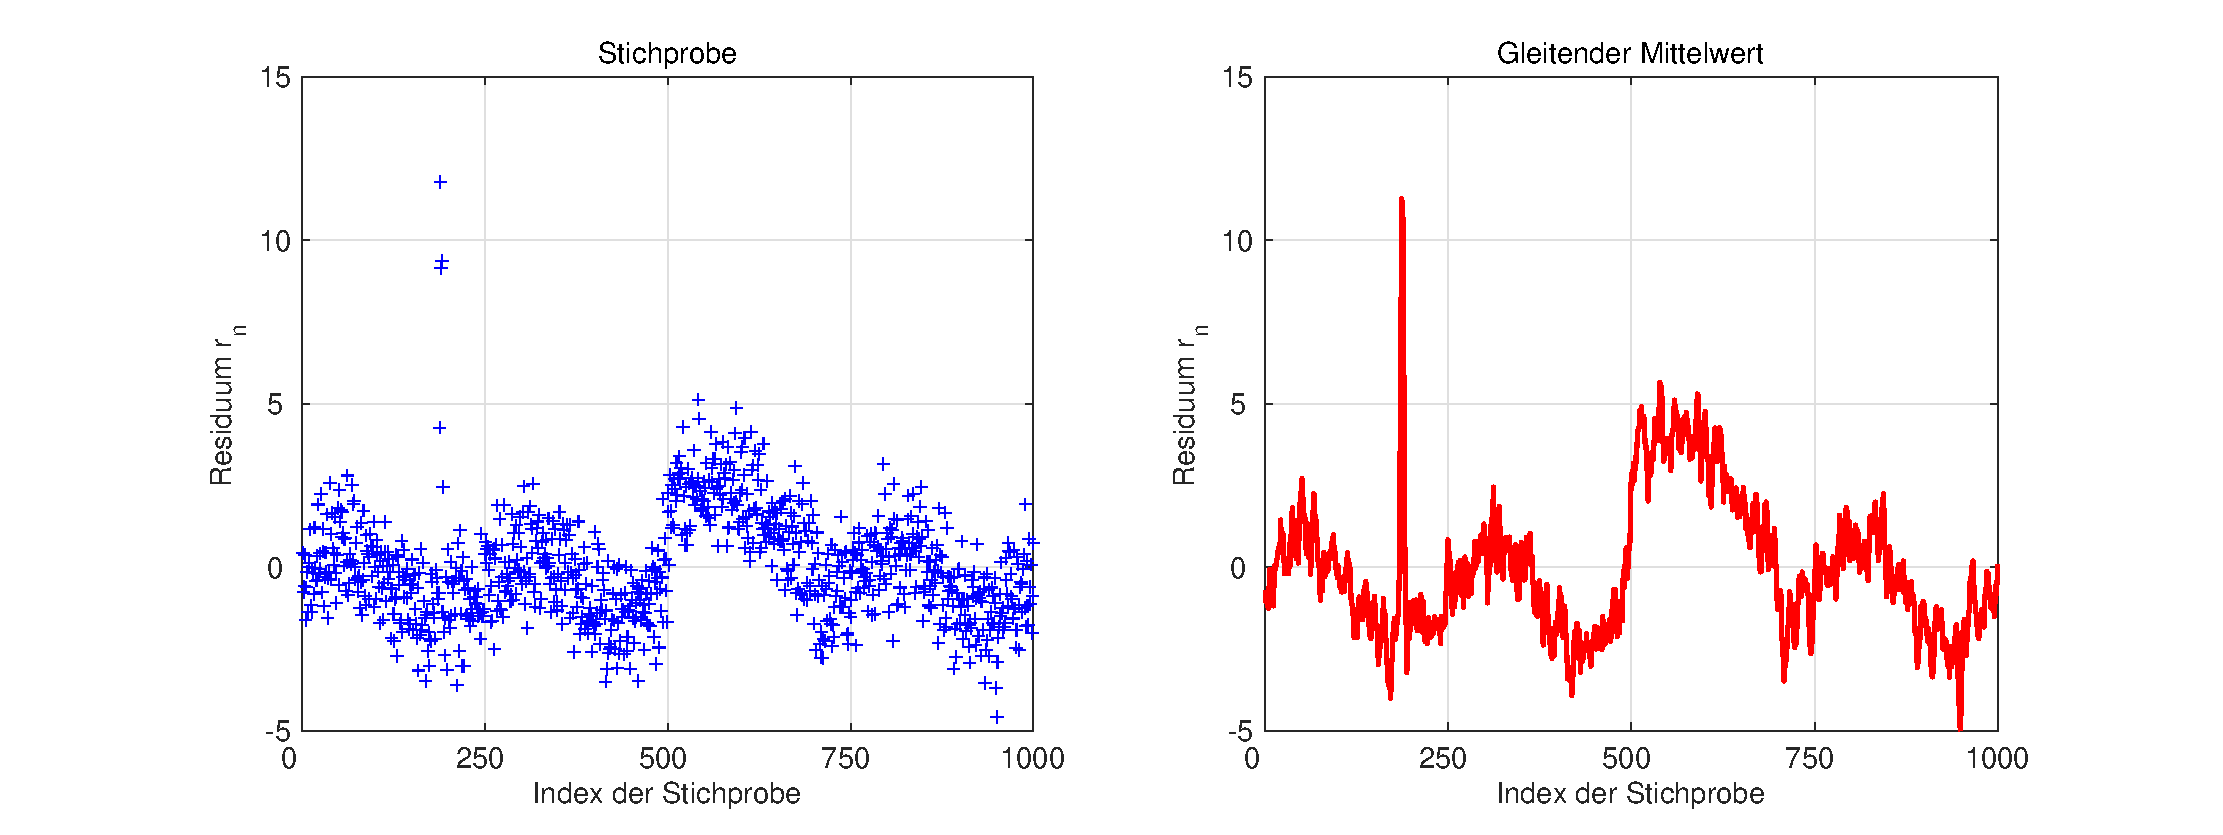
\includegraphics[width=1\textwidth]{Kapitel12/Bilder/image16}}
  \caption{Reststreuungen in der zeitlichen Reihenfolge der Stichprobenaufnahme}
  \label{fig:Residuenanalyse3}
\end{figure}

\noindent Bereits bei einem einfachen Plot der Stichprobe \"{u}ber dem Stichprobenindex wird offensichtlich, dass der Prozess, dem diese Stichprobe entnommen wurde, nicht als station\"{a}r bezeichnet werden kann. Zur Minimierung der Streuung kann ein gleitender Mittelwert \"{u}ber die Stichprobe gebildet werden. In diesem Fall werden f\"{u}nf aufeinander folgende Werte gemittelt. Nach der Mittelung ist eine langwellige Schwingung deutlicher zu erkennen. Ursache k\"{o}nnte zum Beispiel eine Abh\"{a}ngigkeit von der Fertigungsschicht oder der Lufttemperatur sein. Au{\ss}erdem k\"{o}nnen einige Ausrei{\ss}er, die im Box-Plot der Residuen auff\"{a}llig sind, den Indizes 200 - 204 zugeordnet werden. Hier muss sich eine Analyse der Fertigungs- und Messbedingungen f\"{u}r diese Teile anschlie{\ss}en. Weiterhin ist in dem Bereich der Indizes 500 - 700 ein Sprung zu erkennen, der zum Beispiel auf eine auff\"{a}llige Charge von Zukaufteilen hinweisen kann.\newline

\noindent Diese oder andere Filterfunktionen helfen, Anhaltspunkte f\"{u}r die Ursachen von St\"{o}rungen zu identifizieren. Die Ursache f\"{u}r die St\"{o}rungen k\"{o}nnen mit den Zeitangaben gezielt gesucht werden. Diese Informationen erlauben, Prozessschwankungen zeitlich einzugrenzen und gezielt nach den Ursachen f\"{u}r diese Schwankungen zu suchen.\newline

\noindent Die Residuen k\"{o}nnen mit dem Befehl regstats berechnet werden:

\lstinputlisting[caption = {}]{Kapitel12/mat4.m}

\clearpage

\subsection{Sonderformen der zweidimensionalen Regression}

\noindent In praktischen Aufgabenstellungen wird der Einsatz von Regressionsfunktionen aus verschiedenen Gr\"{u}nden erschwert.

\begin{itemize}
    \item Zusammenh\"{a}nge lassen sich nicht zielf\"{u}hrend mit Polynomen beschreiben
    \item  Ausrei{\ss}er verf\"{a}lschen das Ergebnis ma{\ss}geblich
\end{itemize}

\noindent F\"{u}r beide Einschr\"{a}nkungen werden L\"{o}sungsans\"{a}tze skizziert.

\subsubsection{Nichtlineare Regression}

\noindent Einige technische Aufgabenstellungen der Regression haben die Besonderheit, dass der grunds\"{a}tzliche funktionale Zusammenhang bekannt ist und nur Parameter des funktionalen Zusammenhangs bestimmt werden m\"{u}ssen. Zum Beispiel lautet die Shockley-Gleichung f\"{u}r den Strom durch eine Diode

\begin{equation}\label{eq:twelveonehundredthirtyfive}
I_{D} =I_{s} \cdot \left(e^{\dfrac{U_{D}}{n\cdot U_{T}}} -1\right)
\end{equation}

\noindent Dabei ist $I_{D}$ der Strom durch die Diode, $I_{s}$ der S\"{a}ttigungssperrstrom, $U_{D}$ die an der Diode anliegende S\"{a}ttigungsspannung, n der Emissionskoeffizient und $U_{T}$ die temperaturabh\"{a}ngige Temperaturspannung.\newline

\noindent Da die Physik des Diodenstroms und seine mathematische Beschreibung bekannt sind, ist es zielf\"{u}hrend, dieses Wissen in die Approximation oder Regression einzubinden. Es wird deshalb kein Polynom als Approximationsfunktion verwendet, sondern es wird die Approximationsfunktion verwendet, die sich aus der Physik ergibt.\newline

\noindent Um den Diodenstrom $I_{D}$ als Funktion der anliegenden Spannung $U_{D}$ darzustellen, werden einige Messwerte aufgenommen. Sie sind in Tabelle \ref{tab:twelvefifteen} aufgef\"{u}hrt. 

\begin{table}[H]
\setlength{\arrayrulewidth}{.1em}
\caption{Messung der Strom-Spannungskennlinie f\"{u}r eine Diode}
\setlength{\fboxsep}{0pt}%
\colorbox{lightgray}{%
\arrayrulecolor{white}%
\begin{tabular}{| wc{2cm} | wc{1cm} | wc{1cm} | wc{1cm} | wc{1cm} | wc{1cm} | wc{1cm} | wc{1cm} | wc{1cm} | wc{1cm} | wc{1cm}}
\xrowht{10pt}

\fontfamily{phv}\selectfont\textbf{U$_{D}$ / V} & 
\fontfamily{phv}\selectfont{0} & 
\fontfamily{phv}\selectfont{0.1} & 
\fontfamily{phv}\selectfont{0.2} & 
\fontfamily{phv}\selectfont{0.3} & 
\fontfamily{phv}\selectfont{0.4} & 
\fontfamily{phv}\selectfont{0.5} & 
\fontfamily{phv}\selectfont{0.55} & 
\fontfamily{phv}\selectfont{0.6} & 
\fontfamily{phv}\selectfont{0.65} & 
\fontfamily{phv}\selectfont{0.7}\\ \hline \xrowht{10pt}

\fontfamily{phv}\selectfont\textbf{I$_{D}$ / mA} & 
\fontfamily{phv}\selectfont{0} & 
\fontfamily{phv}\selectfont{0.000} & 
\fontfamily{phv}\selectfont{0.001} & 
\fontfamily{phv}\selectfont{0.005} & 
\fontfamily{phv}\selectfont{0.089} & 
\fontfamily{phv}\selectfont{1.537} & 
\fontfamily{phv}\selectfont{6.385} & 
\fontfamily{phv}\selectfont{26.54} & 
\fontfamily{phv}\selectfont{110.3} & 
\fontfamily{phv}\selectfont{458.3}\\ \hline

\end{tabular}%
}\bigskip
\label{tab:twelvefifteen}
\end{table}

\noindent Es liegen 10 Messungen vor, und es m\"{u}ssen die Parameter S\"{a}ttigungsstrom $I_{S}$, Emissionskoeffizient n und Temperaturspannung $U_{T}$ bestimmt werden. Die Aufgabe ist l\"{o}sbar, hier sogar \"{u}berbestimmt.\newline

\noindent Auch bei der nichtlinearen Regression kann die L\"{o}sung \"{u}ber die Minimierung der Fehlerquadrate erfolgen. Diese Methode f\"{u}hrt aber zu einem nichtlinearen Parameteroptimierungsproblem, das im Allgemeinen nur mit numerischen Optimierungsverfahren gel\"{o}st werden kann. Zur L\"{o}sung wurde hier die MATLAB-Funktion nlinfit verwendet. Als Ergebnis ergeben sich die Parameter $I_{s} = 2 nA$, $U_{T} = 24.7 mV$ und $n = 1.423$.\newline

\noindent Um den Vorteil des Verfahrens darzustellen, werden die Messwerte einerseits \"{u}ber Polynome der Ordnung M = 3 und M = 5 dargestellt, andererseits mit den bestimmten Parametern der Diodengleichung berechnet und zur Approximation verwendet. 

\noindent 
\begin{figure}[H]
  \centerline{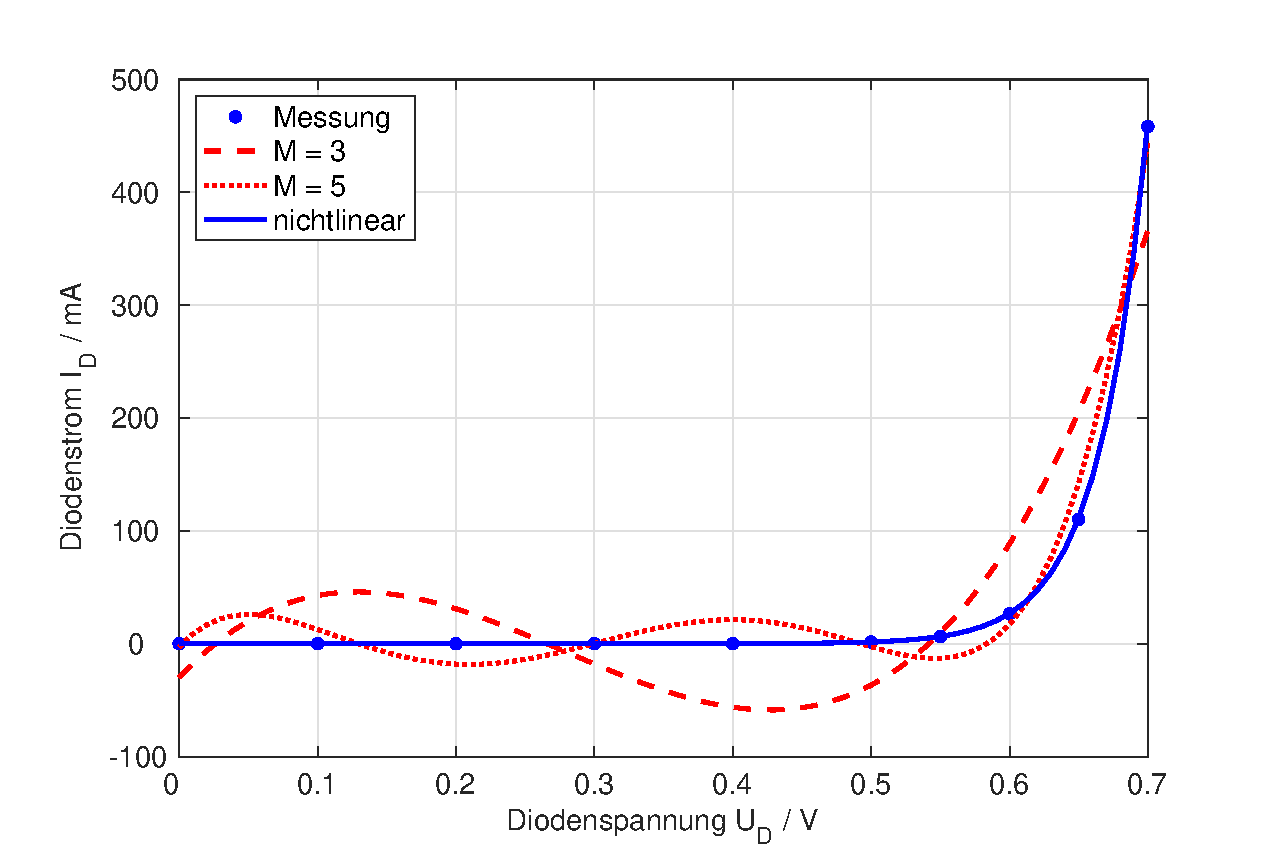
\includegraphics[width=0.5\textwidth]{Kapitel12/Bilder/image17}}
  \caption{Vergleich der Regression von Messwerten mit Polynomen der Ordnung 3 und 5 mit einer physikalisch begr\"{u}ndeten nichtlinearen Regression}
  \label{fig:RegressionNichtlinDiode}
\end{figure}

\noindent Es zeigt sich, dass das Polynom h\"{o}herer Ordnung die Messwerte nicht sinnvoll approximiert, sondern anf\"{a}ngt zu schwingen. Im Gegensatz dazu stellt die physikalisch begr\"{u}ndete, nichtlineare Regression eine gute Approximation dar.\newline

\noindent Die Berechnung in MATLAB erfordert zun\"{a}chst die Definition der nichtlinearen Regressionsfunktion:

\lstinputlisting[caption = {}]{Kapitel12/mat5.m}

\noindent Dann k\"{o}nnen mit der Funktion nlinfit die Parameter der nichtlinearen Regressionsfunktion gesch\"{a}tzt werden.

\lstinputlisting[caption = {}]{Kapitel12/mat6.m}

\noindent Der nichtlineare funktionale Zusammenhang zwischen der Diodenspannung $U_{D}$ und dem Diodenstrom $I_{D}$ wird hier mit einer Exponentialfunktion beschrieben. Alternativ k\"{o}nnte die Diodenspannung transformiert werden, sodass ein linearer funktionaler Zusammenhang entsteht. Mit der Linearisierung des Problems k\"{o}nnen alle statistischen Verfahren zur Berechnung und Bewertung der Regressionsfunktion genutzt werden. Das betrifft s\"{a}mtliche Testverfahren, wie die Berechnung der Konfidenz- und Prognosebereiche sowie die Bewertung der Regressionsg\"{u}te. 

\subsubsection{Behandlung von Ausrei{\ss}ern - Robuste Regression}

\noindent Der in Bild 11.14 dargestellte Datensatz weist einige Ausrei{\ss}er auf. Aufgrund der gro{\ss}en Datenmenge fielen diese Ausrei{\ss}er nicht ins Gewicht. Liegen nur wenige Stichprobenwerte vor, k\"{o}nnen Ausrei{\ss}er das Ergebnis stark verf\"{a}lschen. Um diesen Effekt zu demonstrieren, wird erneut das Beispiel des Temperatursensors zur Messung der \"{O}ltemperatur aufgegriffen. Diesmal wird der Messwert bei $80^{\circ} C$ signifikant ver\"{a}ndert. Es ergeben sich die in Tabelle \ref{tab:twelveseventeen} aufgelisteten Werte.

\begin{table}[H]
\setlength{\arrayrulewidth}{.1em}
\caption{Stichprobe f\"{u}r den Zusammenhang zwischen \"{O}ltemperatur und Ausgangsspannung eines Temperatursensors, Ausrei{\ss}er bei der Messung $80^{\circ} C$ }
\setlength{\fboxsep}{0pt}%
\colorbox{lightgray}{%
\arrayrulecolor{white}%
\begin{tabular}{| wc{3.4cm} | wc{1.8cm} | wc{1.8cm} | wc{1.8cm} | wc{1.8cm} | wc{1.8cm} | wc{1.8cm}}
\xrowht{15pt}

\fontfamily{phv}\selectfont\textbf{Temperatur T / $^{\circ}$C} & 
\fontfamily{phv}\selectfont{0} & 
\fontfamily{phv}\selectfont{10} & 
\fontfamily{phv}\selectfont{20} & 
\fontfamily{phv}\selectfont{30} & 
\fontfamily{phv}\selectfont{40} & 
\fontfamily{phv}\selectfont{50}\\ \hline \xrowht{15pt}

\fontfamily{phv}\selectfont\textbf{Spannung U / V} & 
\fontfamily{phv}\selectfont{2.766} & 
\fontfamily{phv}\selectfont{2.862} & 
\fontfamily{phv}\selectfont{3.005} & 
\fontfamily{phv}\selectfont{3.120} & 
\fontfamily{phv}\selectfont{3.173} & 
\fontfamily{phv}\selectfont{3.411} \\ \hline \xrowht{15pt}

\fontfamily{phv}\selectfont\textbf{Temperatur T / $^{\circ}$C} & 
\fontfamily{phv}\selectfont{60} & 
\fontfamily{phv}\selectfont{70} & 
\fontfamily{phv}\selectfont{80} & 
\fontfamily{phv}\selectfont{90} & 
\fontfamily{phv}\selectfont{100} & 
\\ \hline \xrowht{15pt}

\fontfamily{phv}\selectfont\textbf{Spannung U / V} & 
\fontfamily{phv}\selectfont{3.676} & 
\fontfamily{phv}\selectfont{3.803} & 
\fontfamily{phv}\selectfont\textbf{1.944} & 
\fontfamily{phv}\selectfont{4.188} & 
\fontfamily{phv}\selectfont{4.165} & 
\\ \hline

\end{tabular}%
}\bigskip
\label{tab:twelveseventeen}
\end{table}

\noindent Bild \ref{fig:RegressionRobust} vergleicht die lineare Regression erster Ordnung f\"{u}r die Stichprobe mit und ohne Ausrei{\ss}er.

\noindent 
\begin{figure}[H]
  \centerline{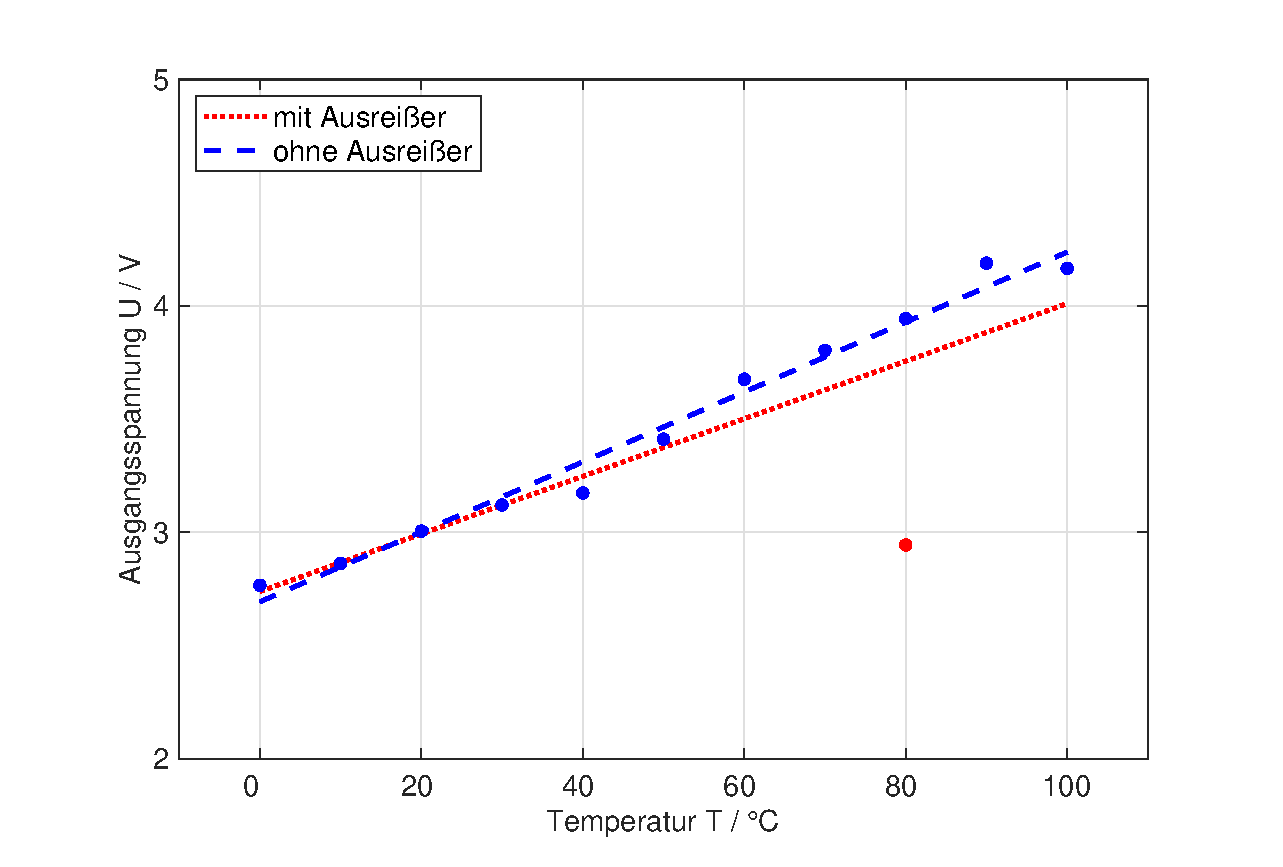
\includegraphics[width=0.5\textwidth]{Kapitel12/Bilder/image18}}
  \caption{Vergleich der Regression von Messwerten mit und ohne Ausrei{\ss}er}
  \label{fig:RegressionRobust}
\end{figure}

\noindent F\"{u}r die Regression dieser Daten stehen in einigen Programmpaketen Funktionen zur Verf\"{u}gung, die die unterschiedlichen Stichprobenwerte unterschiedlich gewichten. Das f\"{u}hrt dazu, dass Ausrei{\ss}er weniger stark in die Summe der Fehlerquadrate eingehen und damit das Regressionsergebnis weniger stark beeinflussen. Bild v stellt diesen Prozess grafisch dar.

\noindent 
\begin{figure}[H]
  \centerline{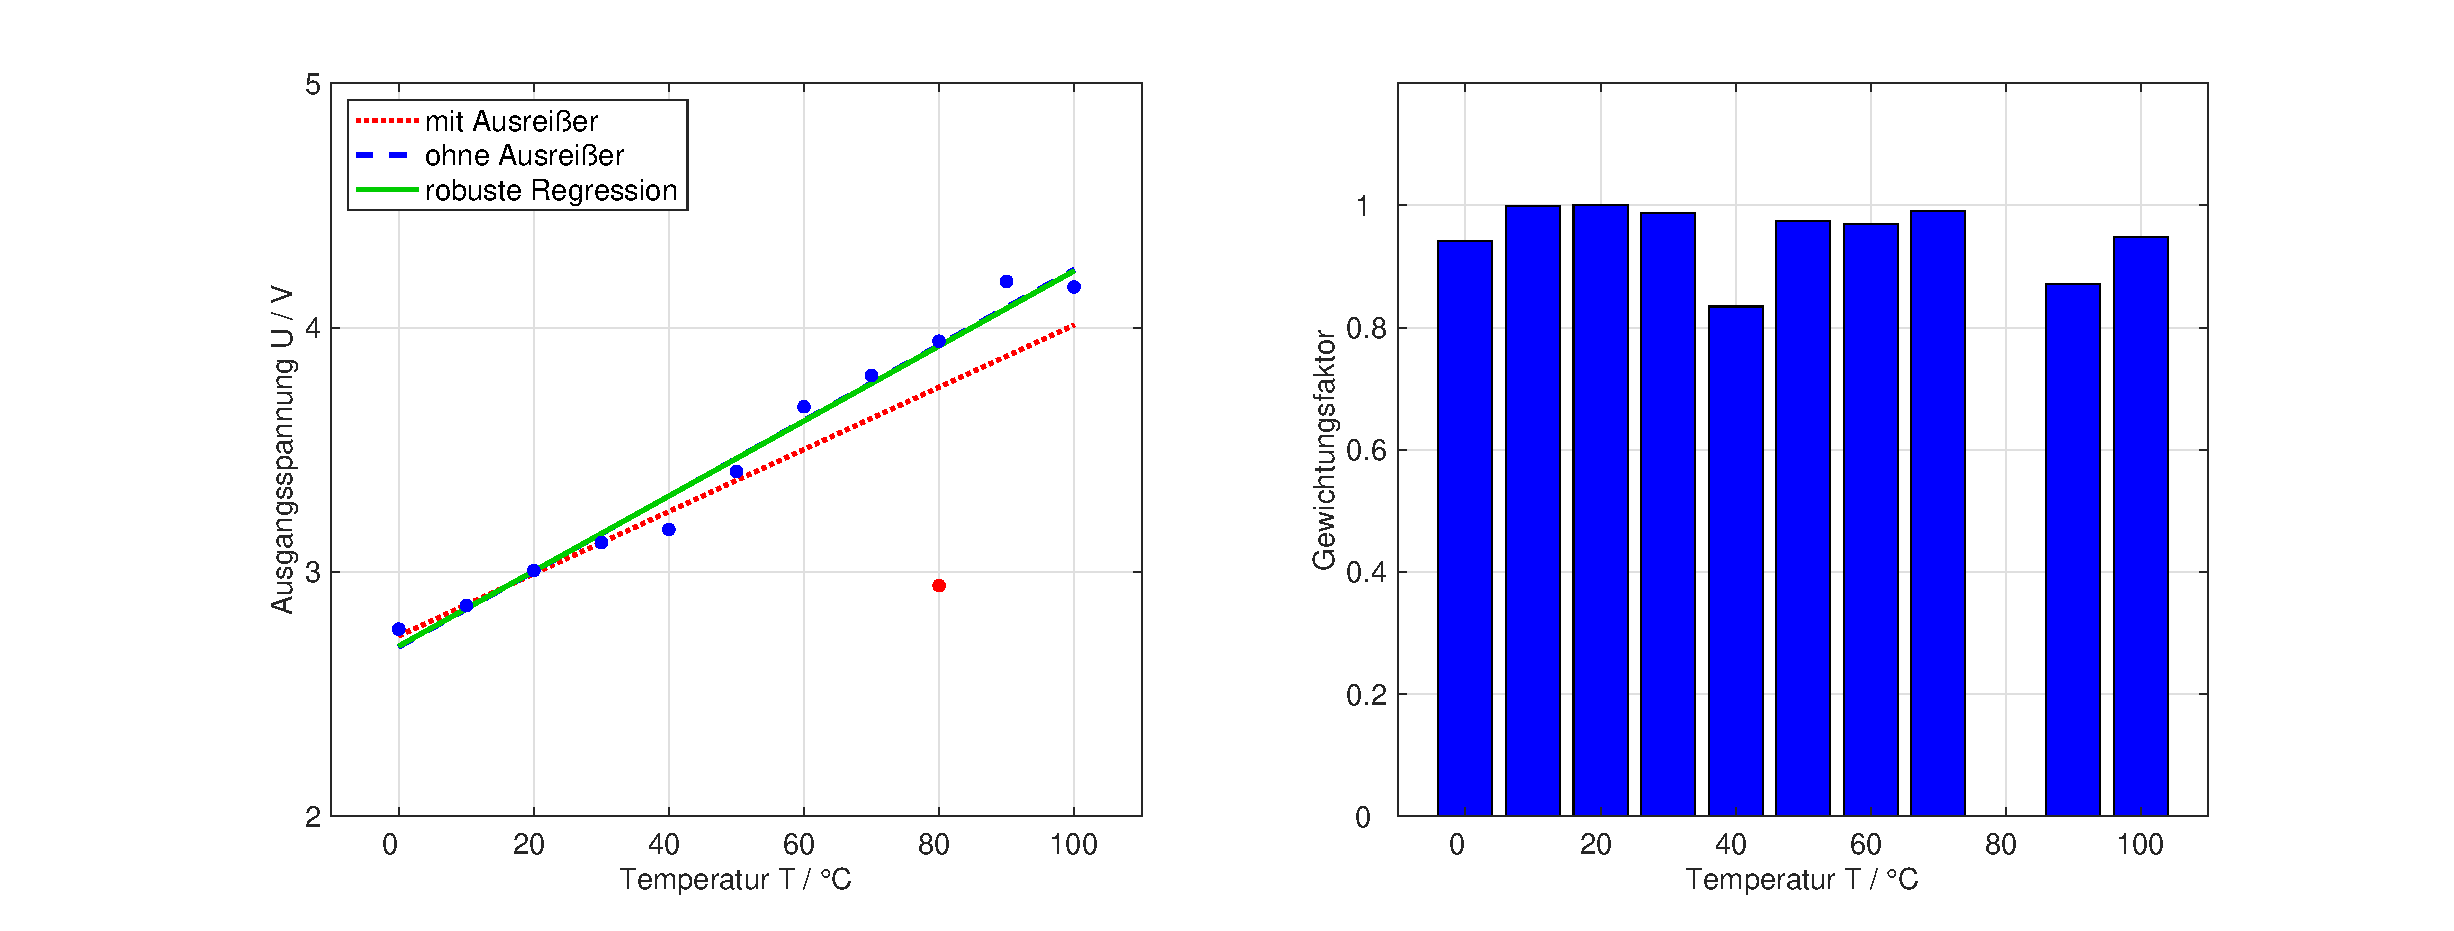
\includegraphics[width=1\textwidth]{Kapitel12/Bilder/image19}}
  \caption{Vergleich der Regression von Messwerten mit und ohne Gewichtung der Ausrei{\ss}er und Darstellung der Gewichtungsfaktoren}
  \label{fig:RegressionRobust2}
\end{figure}

\noindent Es wird deutlich, dass der Messwert bei 80 $^\circ$C mit einem Gewichtungsfaktor nahe null multipliziert wird, sodass dieser Messwert praktisch nicht in das Regressionsergebnis eingeht. Dadurch wird die urspr\"{u}ngliche Regressionsgerade wieder erreicht. 

\noindent Die Gewichtungsfaktoren werden dabei iterativ bestimmt. Als Bewertungskriterium werden die Residuen herangezogen. Je gr\"{o}{\ss}er das Residuum ist, desto weniger stark wird die entsprechende Stelle der Stichprobe zur Berechnung der Regressionsfunktion gewichtet. Dieses Vorgehen ist auch an der Darstellung der Gewichtungsfaktoren in Bild \ref{fig:RegressionRobust2} zu erkennen. Der Ausrei{\ss}er bei 80 $^\circ$C hat praktisch kein Gewicht. Auch die Stichprobenwerte bei 40 vC und 90 $^\circ$C haben ein reduziertes Gewicht, weil sie vergleichsweise stark von der Regressionsfunktion abweichen.

\noindent MATLAB bietet mit dem Befehl robustfit eine M\"{o}glichkeit, eine robuste Regression durchzuf\"{u}hren und zu bewerten.

\clearpage

\subsection{Literatur}

\begin{tabular}{|p{0.6in}|p{5.6in}|} \hline 
[Krey91] & Kreyszig, Erwin: Statistische Methoden und ihre Anwendungen\newline 4., unver\"{a}nderter Nachdruck der 7. Auflage\newline Vandenhoeck \& Ruprecht, G\"{o}ttingen, 1991 \\ \hline 
[Fahr96] & Fahrmeir, Ludwig; Hamerle, Alfred; Tutz, Gerhard: Multivariate statistische Verfahren\newline 2., \"{u}berarbeitete Auflage\newline Walter de Gryter \& Co., Berlin \\ \hline 
[Ross06] & Ross, M. Sheldon: Statistik f\"{u}r Ingenieure und Naturwissenschaftler\newline 3. Auflage\newline Spektrum Akademischer Verlag, M\"{u}nchen, 2006 \\ \hline 
[Hart07] & Hartung, Joachim; Elpelt, B\"{a}rbel: Multivariate Statistik\newline 7., unver\"{a}nderte Auflage\newline R. Oldenbourg Verlag, M\"{u}nchen / Wien \\ \hline 
[Papu01] & Papula, Lothar: Mathematik f\"{u}r Ingenieure und Naturwissenschaftler Band 3\newline 4., verbesserte Auflage\newline Vieweg Teubner, Braunschweig / Wiesbaden, 2008 \\ \hline 
\end{tabular}